\chapter{Non-parametric Bayesian State Space Estimator}

% In this chapter
In both Chapters 3 and 4, we demonstrated that it is feasible to learn a POMDP policy from human teachers. Further,
by adding a simple binary reward function we were able to take into consideration the quality of these demonstrations. 
provided by the teachers. With this, we showed that our Reinforcement Learning extension, RL-PbD-POMDP was able to 
yield improved policies even when provided with a limited number of demonstrations taken from the worst teachers.

Both tasks from the previous two chapters (search for wooden block on a table and peg-in-hole) fall into 
the category of goal oriented \textbf{active-localisation}. In general, the localisation problem consists of estimating 
position parameters given noisy observations whereas active-localisation refers to a policy which actively takes actions to 
acquire information to decrease the uncertainty of the position estimate. In localisation, the model 
of the world also known as the \textbf{map} is considered \textbf{prior knowledge}. This assumption constrains localisation 
to an environment in which schematics exist and can be used 
as the world model such as in the case of offices and buildings. If the map is not known a priori, then Simultaneous Localisation And Mapping (\textbf{SLAM}) algorithms have to be used instead
of localisation. Typically, the map consists of a set of features also known as landmarks which can be identified by sensors, 
and SLAM algorithms maintain a filtered joint probability distribution over both the agent's and features' position which is updated in accordance to a generic 
Bayesian State Space Filter (BSSF) (see Figure \ref{fig:baysian_filter} on page \pageref{fig:baysian_filter}).

In this Chapter, we consider an agent tasked with searching for a set of objects on a \textit{Table} world (see Figure \ref{fig:Figure1}), 
in which exteroceptive feedback is extremely limited. The agent can only sense an object after making physical 
contact with it (bumping into it). The agent's uncertainty of its location and that of the object is encoded by probability distributions $P(\cdot)$, which 
at initialisation are known as the agent's prior beliefs.

Figure \ref{fig:Figure1} illustrates a particular instance of the agent's beliefs. The agent is currently located in the 
bottom  table and has only a limited knowledge of its location, somewhere near the right edge of the table. 

\begin{figure}
  \centering
  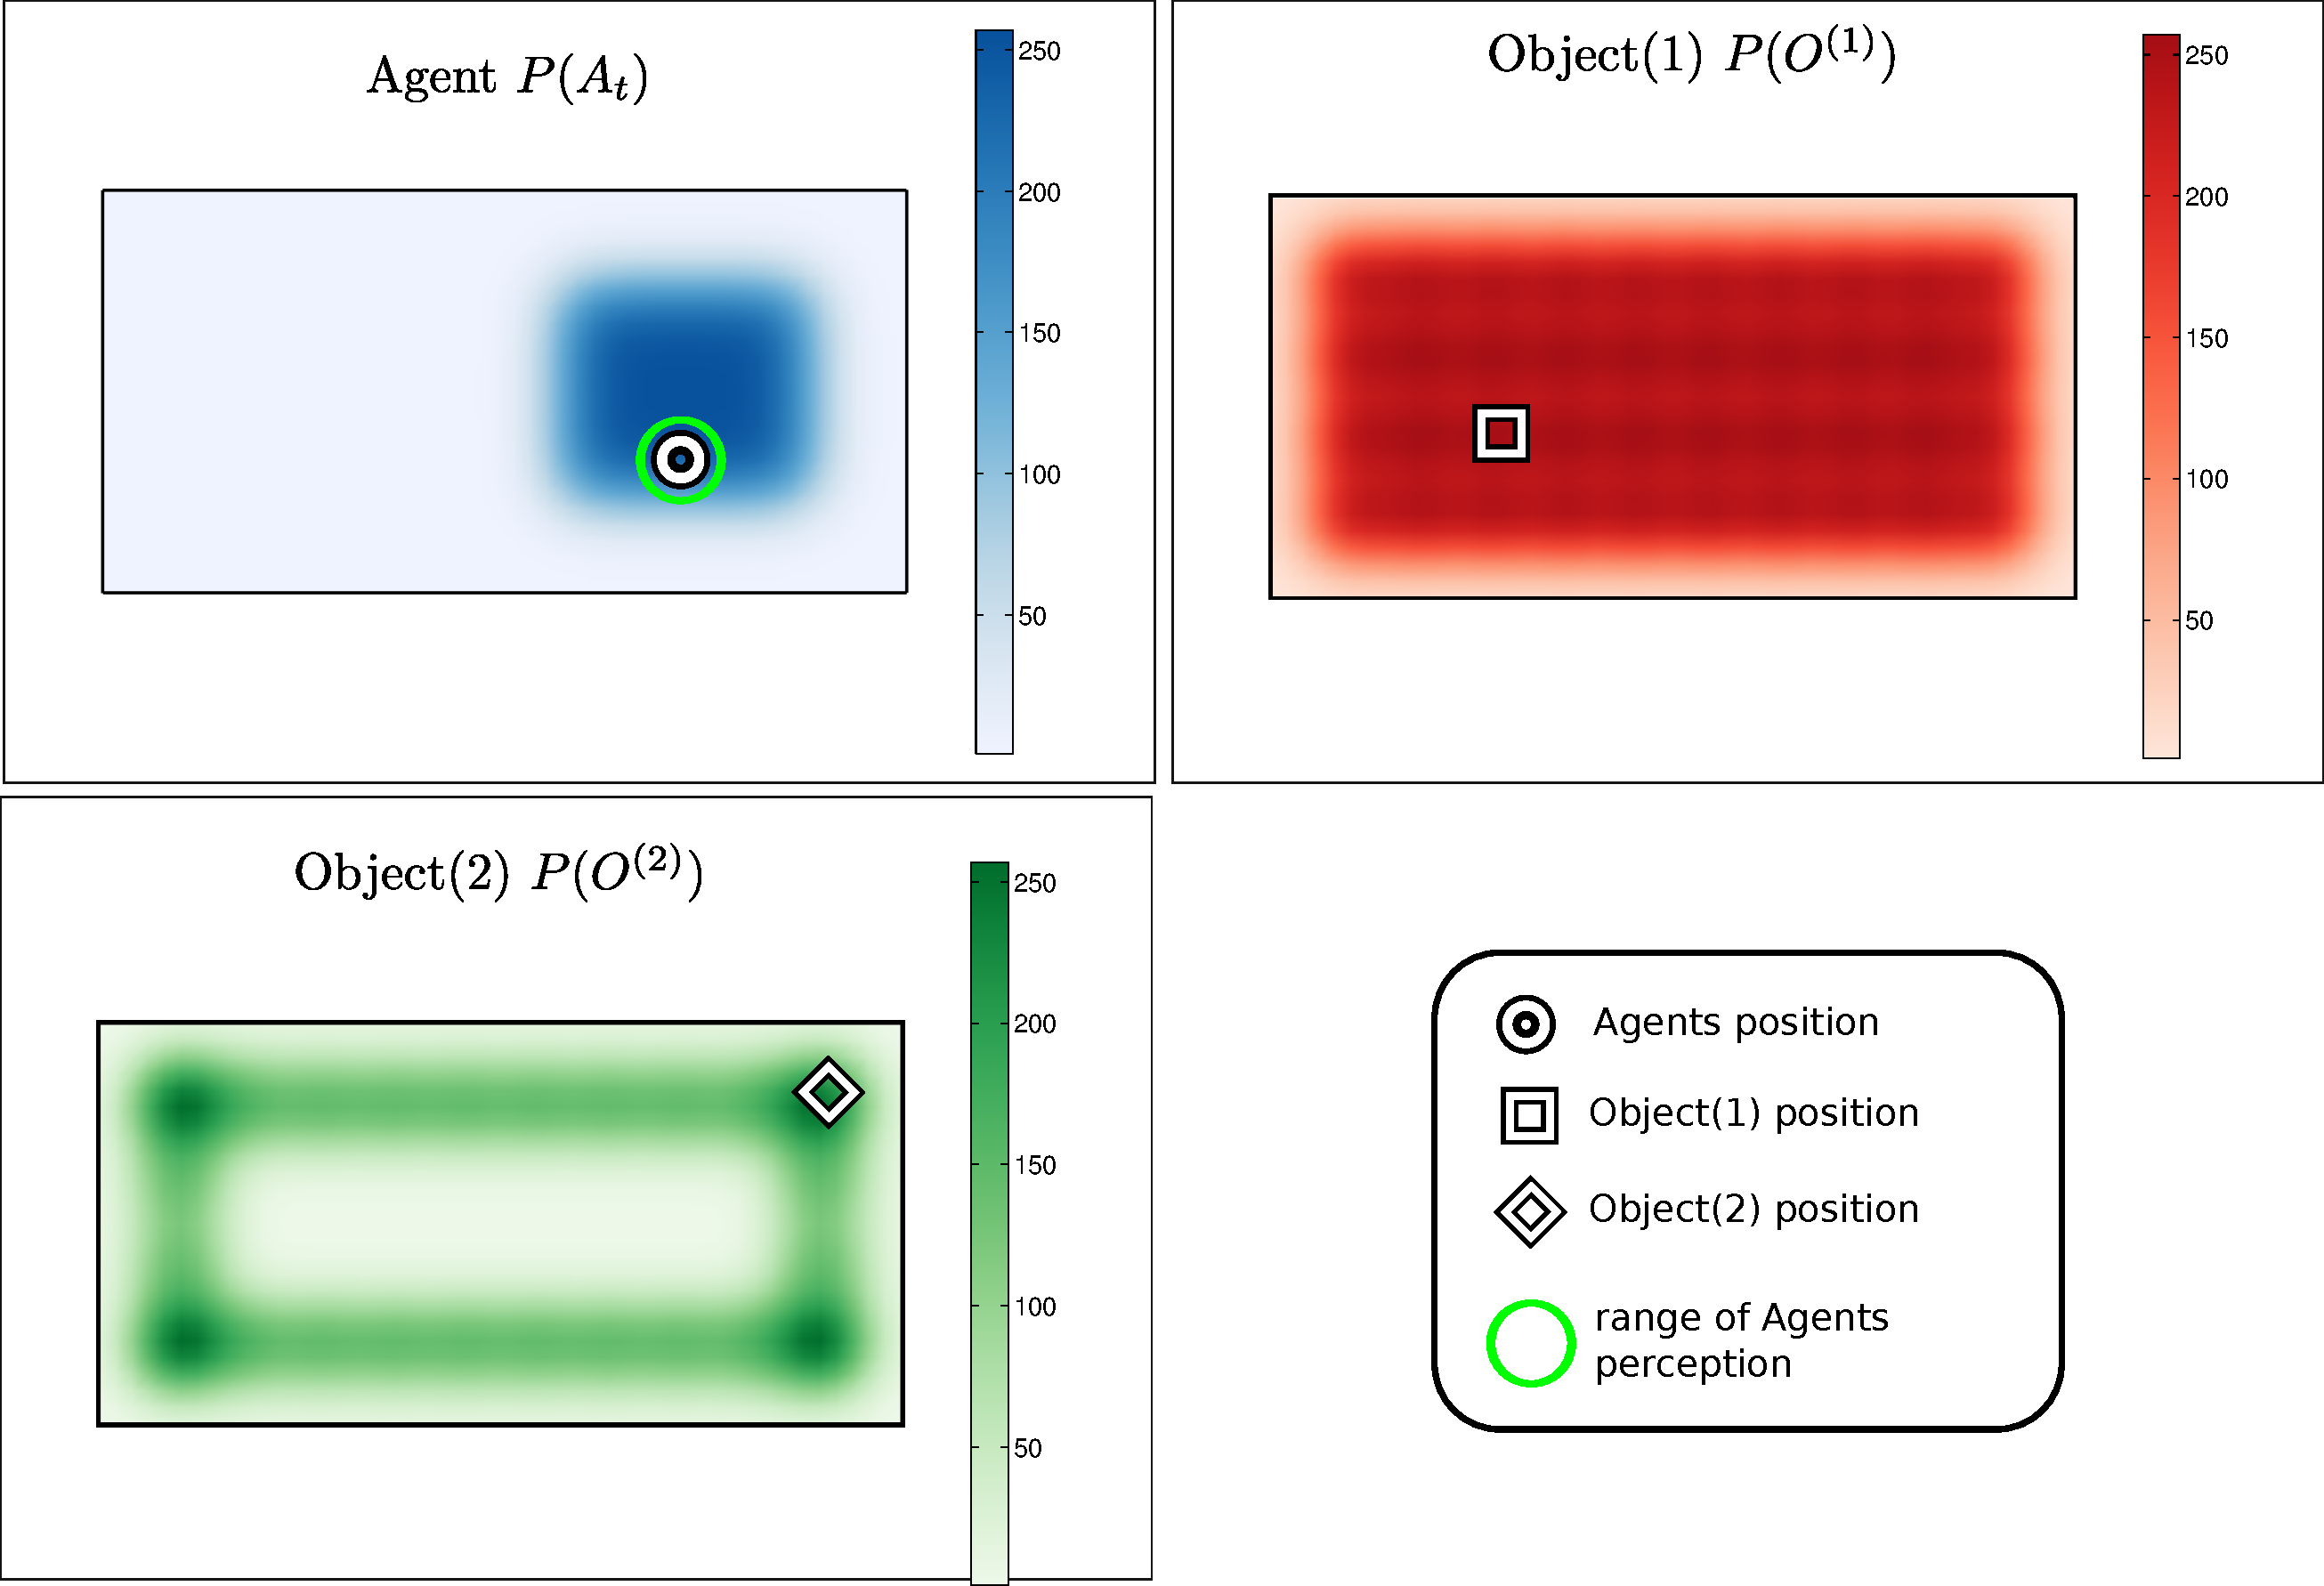
\includegraphics[width=0.95\linewidth]{./ch5-MLMF/Figures/Figure1.pdf}
  \caption{ \textit{Table Environment} Table World (delimited by the black rectangle), viewed from above, and the agent's beliefs. 
  There are three different probability density functions present on the table. 
  The blue represents the believed location of the agent, the red and green probability distributions are associated with object 1 and 2.
  The white shapes in each figure represent the true location of each associated object or agent.}
  \label{fig:Figure1}
\end{figure}
\vspace*{0.6cm}

%	2) Current draw back of all SLAM methodologies 
As the agent explores the world, it integrates all sensing information at each time step and updates its prior beliefs to posteriors
(the result of the prior belief after integrating motion and sensory information).
All current SLAM methods are limited in that they only consider uncertainty induced by sensing inaccuracy inherent in 
the sensor and motion models. In our setting as the sensory information is strictly haptic, we can confidently assume no measurement noise. 
In the search task illustrated in Figure \ref{fig:Figure1}, the beliefs and sparse measurement information available to the agent are 
the source of the uncertainty which is, the absence of positive object measurements. 
This is known as \textbf{negative information} \cite[p.313]{Thrun_Burgard_Fox_2005} \cite{Thrun02particlefilters,negative_info_markov_localisation}. 
Thus SLAM methodologies which use the \textbf{Gaussian error} between the predicted and estimated position of features, such as in the case 
of EKF-SLAM and Graph-SLAM, will not work well in this setting. 

{\quote \textit{The EKF SLAM algorithm, [...], can only process positive sightings of landmarks. It cannot process negative information
that arises from the absence of landmarks. } -Probabilistic Robotics \cite[p.313]{Thrun_Burgard_Fox_2005}-}\\[0.01cm]

In addition to the negative sensing information, the original beliefs depicted in Figure \ref{fig:Figure1} are \textbf{non-Gaussian}
and \textbf{multi-modal}. We make \textbf{no assumption} regarding the form the beliefs can take. This implies that the joint distribution 
can no longer be parameterised by a Multivariate Gaussian. 
This is an assumption made in many SLAM algorithms, notably EKF-SLAM, and allows for a closed form solution to the state estimation problem. Without the Gaussian assumption 
no closed form solution to the filtering problem is feasible. 
Using standard non-parametric methods (Kernel Density, Gaussian Process, Histogram,...) to represent or estimate the joint distribution becomes
unrealistic after a few dimensions or additional map features. 
FastSLAM could be a potential candidate, however as it parameterises the position uncertainty of the agent by a particle filter and each
particle has its own copy of the map, the memory demand will become significant.  For planning purposes we would also want to have a 
single representation of the marginals. Figure \ref{fig:ch5_assmuptions} summarises the desirable attributes and assumptions for our filter.

\begin{figure}
\centering
\begin{tikzpicture}    
\node [white_box] (box){%
\begin{minipage}{0.95\textwidth}
\begin{itemize}
  \item Non-Gaussian joint distribution, no assumptions are made with respect to its form.
  \item Mostly negative information available (absence of positive sightings of the landmarks).
  \item Joint distribution volume grows exponentially with respect to the number of objects and states.
  \item Joint distribution volume is dense, there is a lot of uncertainty.
\end{itemize}
\end{minipage}

};
\node[fancytitle, right=10pt] at (box.north west) {Attributes \& Assumptions};
\end{tikzpicture}%
\caption{Assumptions and attributes which have to be fulfilled by our Bayesian State Space Filter. }
 \label{fig:ch5_assmuptions}
\end{figure}

\textit{The main contribution of our work and the importance to the field of Artificial Intelligence} 

An accurate estimate of the agent's belief space is a necessary precondition before planning or reasoning can be carried out.
In a wide range of Artificial Intelligence (AI) applications the agent's beliefs are discrete. This non-parametric representation
is the most unconstraining but comes at a cost. The parameterisation of the belief's joint distribution grows at the rate of a double exponential.
We propose a Bayesian state estimator which delivers the same filtered beliefs as a traditional filter but without explicitly parametrising the 
joint distribution. Through the memorising of the measurement likelihood functions having been applied on the joint distribution 
and by taking advantage of their structure, we achieve a filter which grows linearly as opposed to exponentially 
in both time and space complexity. We refer to our novel filter as the Measurement Likelihood Memory Filter (MLMF) 
it keeps track of the history of measurement likelihood functions, referred to as the memory, which 
have been applied on the joint distribution.
The MLMF filter allows to efficiently process negative information. To the authors knowledge there has been little
research on the integration of negative information in a SLAM setting. Previous work considered the case of active localisation \cite{NegInfoFurtherStudies}.
The incorporation of negative information is useful in many contexts and in particular in Bayesian Theory of Mind \cite{Bake_Saxe_Tene_2011},
where the reasoning process of a human is inferred from a Bayesian Network and in our own work \cite{deChambrier2013} where we model the 
search behaviour of a intentionally blinded human. In such a setting much negative information is present and an efficient belief filter is required. 
Our MLMF is thus applicable to the SLAM \& AI community in general and to the cognitive community which models human or agent behaviours through 
the usage of Bayesian state estimators.

By using this new representation we implement a set of passive search trajectories through the state 
space and demonstrate, for a discretised state space, that our novel filter is optimal with respect to the Bayesian criteria (the successive
filtered posteriors are exact and not an approximation with respect to Bayes rule). We provide an analysis of the space and time complexity of 
our algorithm and prove that it is always more efficient even when considering worst case scenarios.
Lastly we consider an Active-SLAM setting and evaluate the effect of how constraining the size of the number of memorised likelihood 
functions impacts the decision making process of a greedy one-step look-ahead planner.

\section{Outline}

% \hyperref[ch3:background]{\ref{ch3:background}   Background}

The remaining part of this Chapter is structured as follows:


\begin{itemize}
 \item \hyperref[ch5:background]{\ref{ch5:background} Background}: Review of three prominent SLAM algorithms
 and their assumptions and an overview of active-localisation and exploration methods used with SLAM.
 \item \hyperref[ch5:BSSE]{\ref{ch5:BSSE} Bayesian State Space Estimation}:  Introduction to EKF-SLAM and why it 
  is not suitable when mostly negative information is available. Description 
 of the Histogram-SLAM algorithm and the assumptions which can be exploited.
 \item \hyperref[ch5:MLMF]{\ref{ch5:MLMF} Measurement Likelihood Memory Filter}:
 Mathematical derivation of the MLMF, time and space complexity evaluation and extension to 
 the scalable-MLMF.
 \item \hyperref[ch5:evaluation]{\ref{ch5:evaluation} Evaluation}
 We numerically evaluate the time complexity of the scalable-MLMF and check its assumptions.
 We investigate the filter's sensitivity with respect to its parameters in an Active-SLAM setting.
 \item \hyperref[ch5:conclusion]{\ref{ch5:conclusion} Conclusion}
 \item \hyperref[ch5:appendix]{\ref{ch5:appendix} Appendix}
\end{itemize}

\section{Background}\label{ch5:background}

\subsection{SLAM}

% Introduction of SLAM
Estimating the location or state parameters of a mobile agent whilst simultaneously building a map of the environment has been
regarded as one of the most important problems to be solved for agents to achieve true autonomy. It is a necessary precondition for 
any agent to have an estimation of the world at its disposal which accurately encompasses all knowledge and related uncertainties. 
There has been much research surrounding the field of Simultaneous Localisation And Mapping (SLAM) which branches out into a wide variety of sub-fields 
dealing with problems from building accurate noise models of the agent sensors \cite{Plagemann07gaussianbeam}, to determining which environmental 
feature caused a particular measurement, also known as the data association problem \cite{DataAssociation2003} and many more. 

% Why does SLAM Work

Although the amount of research might seem overwhelming at first view, all current SLAM methodologies are founded on a single principle; 
the uncertainty of the map is correlated through the agent's measurements. When an agent localises itself (by reducing position uncertainty)
all previously landmarks have their uncertainty reduced since the uncertainty is correlated with that of the agent's uncertainty.

% The three main pillar of SLAM algorithm and their respective draw backs

There are three main paradigms to solving the SLAM problem. The first is EKF-SLAM (Extendend-Kalman Filter) \cite{SLAM_part1}.
EKF-SLAM models the full state, being the agent's parameters and environmental features, by a Multivariate Gaussian distribution. 
The uncertainty of each individual feature is parametrised by a mean (expected position of the feature) and covariance 
(how much uncertainty there is about the position of the feature).

The second approach is Graph-SLAM \cite{TutGraphSLAM}. Graph-SLAM estimates the full path of the agent and considers every measurement to 
be a constraint on the agent's path. It is parameterised by the canonical Multivariate Gaussian. At each time step a new row and column 
is added to the precision matrix which encodes landmarks which have been observed as constraints on the robot's position.
At predetermined times, a nonlinear sparse optimisation is solved to minimise all the accumulated constraints on the robot's path.

The third method is FastSLAM \cite{FastSLAM}. FastSLAM exploits the fact that if we know the position of the agent with 
certainty all landmarks become independent. It models the distribution of the agent's position by a particle filter. Each particle
has its own copy of the map and updates all landmarks independently which is the strength of this method. 
However, if many particles are required each must have its own copy of the map. 
It is beyond the scope of this chapter to provide a detailed review of these  three paradigms and the reader is referred to \cite{Thrun_Burgard_Fox_2005}, \cite{SLAM_HBR}.

\subsection{Active-SLAM \& Exploration}

Active-SLAM refers to a decision theoretic process of choosing control actions so as to actively 
increase the convergence of the map. It is used in conjunction with exploration of an unknown environment
in a SLAM setting. The two steps of this process are: (i) generate a set of 
candidate destination positions, (ii) evaluate these positions based on a utility function. The utility  
is a trade off between reducing the uncertainty of the map or reducing the uncertainty
of the agent's position.

Most approaches use a two-level representation of the map in an exploration setting. At the lower level
there is the chosen (landmark-based) SLAM filter and at the higher level a coarser representation of the world.
Such representations can be occupancy grids \cite{Thrun_grid_based_1996} which encode either occupied and free space
or a topological representation \cite{Kollar_2008_Exploration_SLAM}.

Early and current approaches to selecting candidate exploratory locations are based on evaluating 
Next-best-view \cite{Navigation_strategires_for_exploring_indoor_environments} locations. Next-best-view points are 
sampled around \textit{free edges} which are at the horizon of the known map (\textit{frontier} regions). 
In such a setting only target points are generated, not the full trajectory. Probabilistic Road Map (PRM) \cite{PRM_1996}
based methods have been used as planners to reach desired target locations, such as in \cite{RRT-SLAM}, where a Rapidly
Exploring Random Trees (RRT) is combined with FastSLAM. In \cite{ActivePosSLAM}, paths to \textit{frontier} regions are computed
via PRM  on a occupancy grid map and at the lower level they use Pose-SLAM (synonym for Graph-SLAM).

An alternative approach taken to generating candidate locations is the specification of high level macro actions, they being either 
\textit{exploratory} or \textit{revisiting} actions as is the case in \cite{stachniss05robotics}. Macro actions
reduce the costly evaluation of actions, especially in the case of FastSLAM, which requires propagating the filter 
forward in time so as to infer the information gain of each action.

The last approach is to solve the planning problem through formulating it as  Partially Observable Markov Decision Process (POMDP) \cite{Ross08onlineplanning}. 
However all methods take an approximation of the POMDP and consider a one time step planning horizon \cite[p.37]{GeorgiosLidoris}.

There are many ways of generating actions or paths, however their utility is nearly all exclusively based on the \textit{information gain}, 
which is the estimated reduction of entropy a particular action or path would achieve. A few utilities use f-measures such as the Kullback-Leibler divergence. 
Evaluation of different utility metrics are presented in \cite{Active_SLAM_Uncertainty_compar,tovar_planning,KL_SLAM_exploration_PF}.



\section{Bayesian State Space Estimation}\label{ch5:BSSE}

Bayesian State Space Estimation (BSSE) focuses on incorporating observations to update a prior distribution over
the state space to a posterior distribution through the application of Bayes probability rules. The agent's random variable, $A$, 
is associated with the uncertainty of its location in the world, the same holds for the object(s') random variable(s), $O$. 
Given a sequence of actions and observations, $\{u_{1:t},y_{0:t}\}$ (subscript $0:t$ is the set from the time $t=0$ to the current time, $t=t$), 
algorithms of the BSSE family incorporate this information to provide an estimate:

\begin{equation}
 P(A_t,O|Y_{0:t},u_{1:t}) 
 \label{eq:joint}
\end{equation}

This is know as the filtering problem where all past information is incorporated to estimate the current state.  

\begin{figure}
\centering
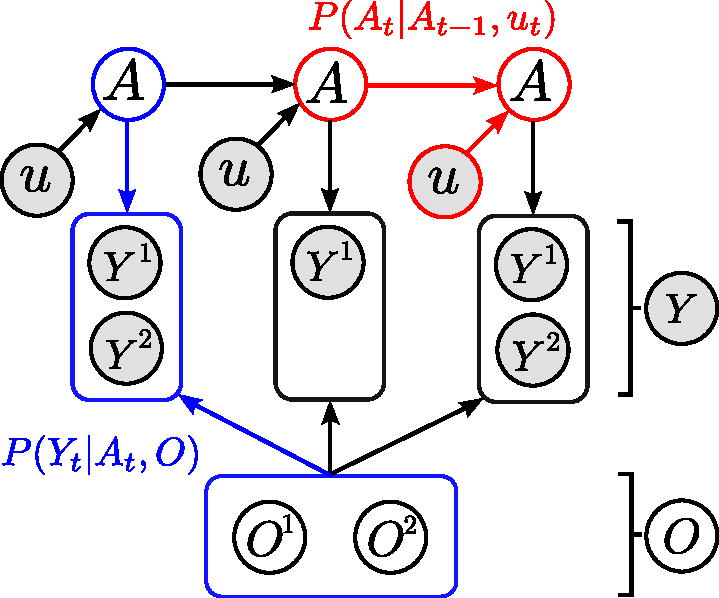
\includegraphics[width=0.8\textwidth]{./ch5-MLMF/Figures/Figure2.pdf}
\caption{Directed graphical model of dependencies between the agent(A), objects(O), sensing(Y) and action(u) random variables. Each 
object, $O^{(i)}$ is associated with one sensing random variable $Y^{(i)}$. The overall sensing random variable is $Y = \left[Y^{(1)},\dots,Y^{(M-1)}\right]^{\mathrm{T}}$,
where $M$ is the total number of agent and object random variables in the filter. 
For readability we have left out the time index $t$ from $A$ and $Y$. Since the objects are static, they have no temporal process associated with 
them thus they will never have a time subscript. The two models necessary for filtering are the motion model $P(A_t|A_{t-1},u_t)$ (red) and measurement model
$P(Y_t|A_t,O)$ (blue).}
\label{fig:bayesian_sse_dag}
\end{figure}

In Figure \ref{fig:bayesian_sse_dag} we depict the general Bayesian Network (BN) of a BSSE. The BN conveys two types of
information, the dependence and independence relations between the random variables in the graph which can be established
through \textit{d-separation} \cite{BayesBall}, see Figure \ref{fig:ch5_dseperation}. Any joint probability distribution 
whose factorisation  respects the structure of a BN is guaranteed to satisfy all the conditional independence 
statements which can be read from the graph, but the converse with respect to the dependence statements is 
not guaranteed \cite[p.43]{barberBRML2012}. 

The \textbf{conditional dependence} $A \dependent O | Y$ is key to all BSSE and SLAM algorithms. The strength of the dependence 
between the agent and object random variable is governed by the measurement likelihood $P(Y_t|A_t,O)$. If it does not change the 
joint distribution then the agent and object random variables will be independent, $A \independent O$. If they are independent, 
then no information acquired by the agent can be used to infer changes in the object estimates.

%the measurement $Y$ makes both $A$ and $O$
%dependent implying that any decrease of uncertainty will effect both $A$ and $O$. The strength of the dependence between the agent and object
%is dictated by the value function.
%If there is no observation, no information will be exchanged between the two and no decrease of uncertainty can take place.

We next demonstrate the behaviour of the two different parameterisations of the joint distribution of the BN, 
Figure \ref{fig:bayesian_sse_dag}, in the case of the absence of direct sighting of the object by the agent. We first consider a
Multivariate Gaussian parameterisation of the joint distribution, which is known as EKF-SLAM, and 
a different approach which discretises the joint distribution, called Histogram-SLAM.


\begin{figure}
\centering
\begin{tikzpicture}    
\node [white_box] (box){%
\begin{minipage}{0.95\textwidth}
\begin{tabular}{lp{7cm}}
 Conditional independence & \\
 1) $A_{t+1} \independent A_{t-1} | A_t$ 	&  First order Markov property. \\
 2) $A_{t} \independent Y_{t+1} | A_{t+1}$ & Past states do not depend on future observations. \\
 3) $A \independent O | \emptyset$ 	& Agent and object random variables are independent given no observation. \\
 Conditional dependence & \\
  1) $A \dependent O | Y$ 	&  Agent and object random variables will interact with each other given an observation 
\end{tabular}
\end{minipage}

};
\node[fancytitle, right=10pt] at (box.north west) {Dependence \& Independence};
\end{tikzpicture}%
\caption{Dependence and independence relation between the random variables of the BN Figure \ref{fig:bayesian_sse_dag}}
 \label{fig:ch5_dseperation}
\end{figure}

\subsubsection{EKF-SLAM}\label{sec:EKF-SLAM}

In EKF-SLAM the joint density $p(A_{t},O|Y_{0:t},u_{1:t}) = g(x;\mu_t,\Sigma_t)$ is parametrised by a single Gaussian function $g$ with mean,
$\mu_t = \left[\mu_{A_{t}},\mu_{O^{(1)}},\dots,\mu_{O^{(M-1)}}\right]^{\mathrm{T}} \in \mathbb{R}^{3 + 2\cdot (M-1)}$  where the 
random variables are in $\mathbb{R}^2$, and covariance, $\Sigma_t$. The mean value of
the agent $\mu_a = [x,y,\phi]^{\mathrm{T}} \in \mathbb{R}^3$ and those of the objects are $\mu_{O^{(i)}} = [x,y]^{\mathrm{T}} \in \mathbb{R}^2$.

\begin{equation}
\Sigma_t = \begin{bmatrix}
       \Sigma_a & \Sigma_{ao}  \\[0.3em]
       \Sigma_{oa} & \Sigma_o
     \end{bmatrix}
     \in \mathbb{R}^{(3 + 2\cdot (M-1)) \times (3 + 2\cdot (M-1))}
\end{equation}

The $j$'th object measurement is described by range and bearing  $Y^{(j)}_t = [r,\phi]$ in the frame of reference of the agent,
see Figure \ref{fig:belief_update_example} page \pageref{fig:belief_update_example} for an illustration of a measurement update process.
EKF-SLAM assumes that the measurement is corrupted by Gaussian noise, $\epsilon \sim \mathcal{N}(0,R)$,
and this results in a measured likelihood function of the following form:
\begin{equation} \label{eq:lik-measurement}
   p(Y_t|A_t,O_t) = \frac{1}{|2\pi R|^{\frac{1}{2}}} \exp \left( -\frac{1}{2} \big(Y_t - \hat{Y}_t\big)^{\mathrm{T}}R^{-1}\big(Y_t - \hat{Y}_t\big) \right)
\end{equation}
where the covariance, $R$, encompasses the uncertainty in the measurement. The elements of the covariance matrix capture 
the measurement error between the true $Y$ and expected $\hat{Y}$ range and bearing of the object. As the joint distribution 
is parametrised by a single Multivariate Gaussian, a closed form solution to the filtering Equations exists, called the Kalman 
Filter \cite{SLAM_part1}. 

The error between the true and expected measurement $e = (Y_t - \hat{Y}_t)$ is an important part of the application of EKF-SLAM.
In our scenario the agent can only perceive the objects once he enters in direct contact with them. 
This means that the variance of the observation $Y_t$ will be very low and will always be equal to $\hat{Y}$ until a contact occurs. 
To illustrate the problems which this gives rise to, we give an illustration of a 1D search. Figure \ref{fig:EKF-SLAM} shows the 
resulting updates of the beliefs for 4 chosen time segments.

\begin{figure}
\centering
 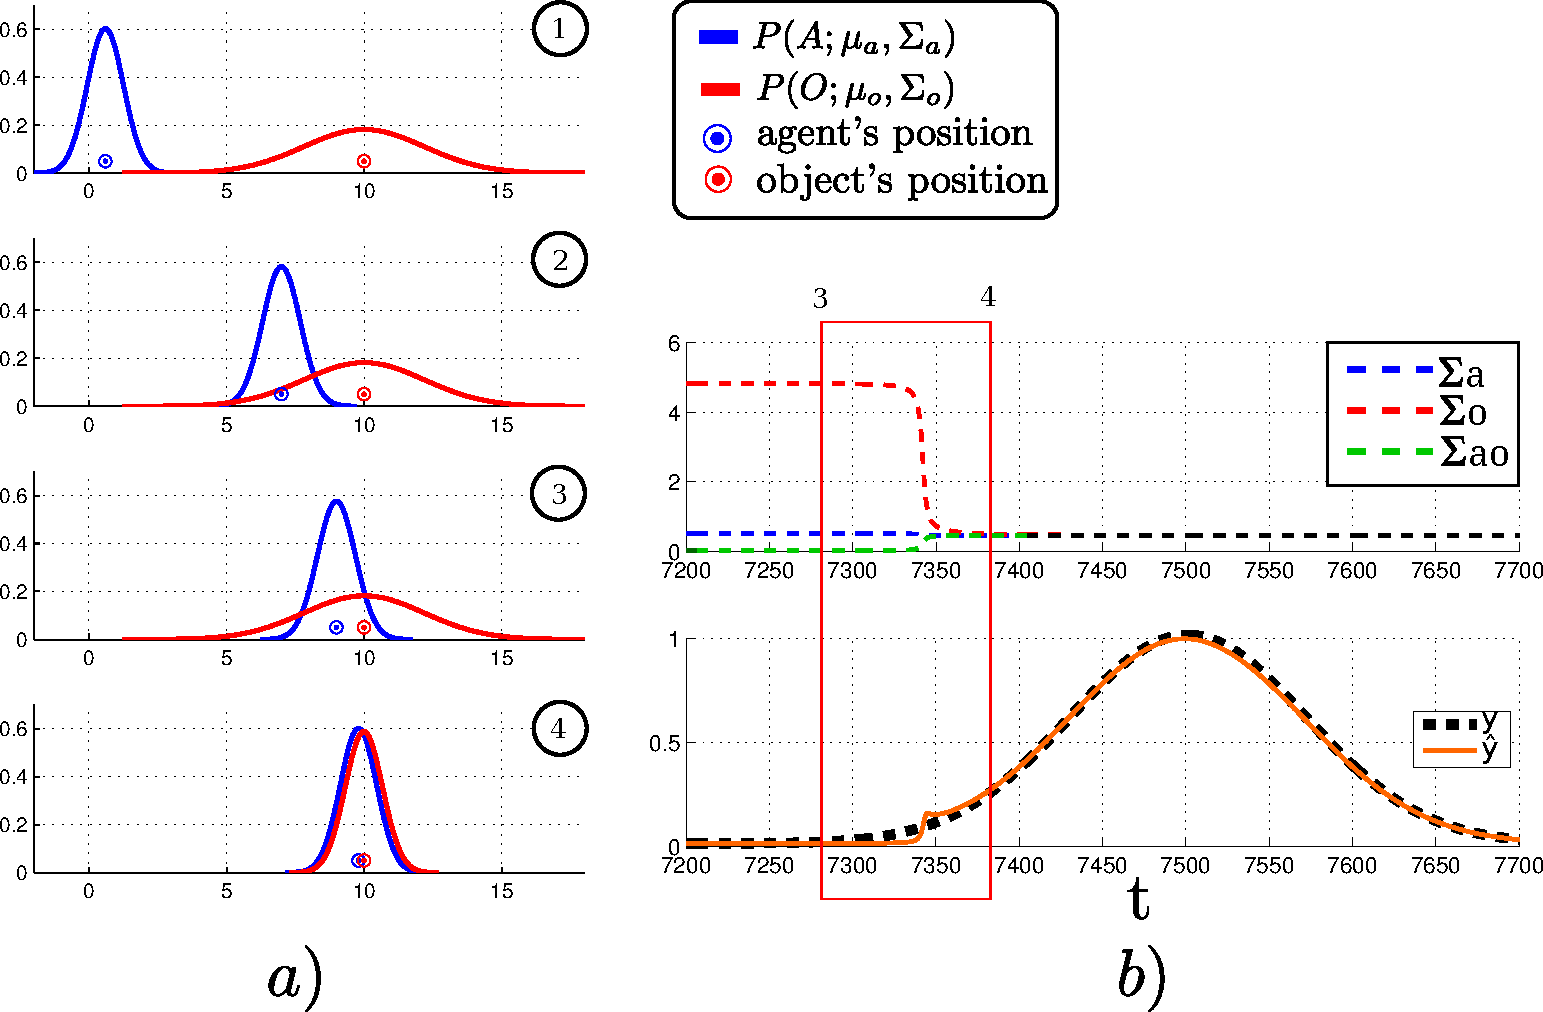
\includegraphics[width=0.9\textwidth]{./ch5-MLMF/Figures/Figure34.pdf}
\caption{\textbf{a)} EKF-SLAM time slice evolutions of the pdfs. 
The temporal ordering is given by the numbers in the top right corner of each plot.
The blue pdf represents the agent's believed location and the circle is the agent's true location. The same holds 
for the red distribution which represents the agent's belief of the location of an object.
\textbf{b)} Evolution of the covariance components of $\Sigma$ over time and true $Y_t$ and expected measurements,  $\hat{Y}_t$. 
$\Sigma_a$ and $\Sigma_o$ are the variances of the agent and object positions and $\Sigma_{ao}$ is the cross-covariance 
term.}
\label{fig:EKF-SLAM}
\end{figure}

As expected we do not get the desired behaviour, which is that the beliefs start updating as soon as they are overlapping, 
see 2nd-3rd temporal snapshot in the Figure. 
Even when most of the belief mass of the agent's location pdf overlaps that of the object pdf, no belief update occurs. 
The multivariate Gaussian parameterisation only guarantees a dependency between the agent and object random variables 
when there is a positive sighting of the landmarks.  This can been seen in Figure \ref{fig:EKF-SLAM} (b),
where the component $\Sigma_{ao}$ is 0 most of the time which implies that $A \independent O | Y$ which is undesirable. 
This confirms that the dependencies present in the structure given by the BN are dependent on the chosen parametrisation.

\subsubsection{Histogram-SLAM}\label{sec:Discrete}

In Histogram-SLAM, the joint distribution is discretized and each bin has a parameter, 
$P(A_t=i,O=j|Y_{0:t},u_{1:t}) = \boldsymbol{\theta}^{(ij)}$, which sums to one, $\sum_{ij} \boldsymbol{\theta}^{(ij)} = 1$. 
For shorthand notation we will write $P(A_t,O|Y_{0:t},u_{1:t})$ instead of $P(A_t=i,O=j|Y_{0:t},u_{1:t})$.
The probability distribution of the agent's position is given by marginalising the object random variable:
\begin{align}
 &P(A_t|Y_{0:t},u_{1:t})    = \sum\limits_{j=1}^{|O|} P(A_t,O|Y_{0:t},u_{1:t}) \label{eq:agent_marginal} \\
 &P(A_t=1|Y_{0:t},u_{1:t})  = \sum\limits_{j=1}^{|O|} \boldsymbol{\theta}^{(1j)}
\end{align}
The converse holds true for the object's marginal over its believed position. Figure \ref{fig:histogram_joint} illustrates 
the joint distribution of both the agent and the object random variable. For ease of notation we use the shorthand $P(A)$
for $P(A_t|Y_{0:t},u_{1:t})$. The 1D world of the agent and object is discretised to 10 states, producing 
a joint distribution with 100 parameters!
For a state space of $N$ bins, $i=1...N$, and there is a total of $M$ random variables (one agent and $M-1$ objects)
and the joint distribution has $N^{M}$ parameters. This exponential increase renders Histogram-SLAM intractable
with this parameterisation.

\begin{figure}
 \centering
 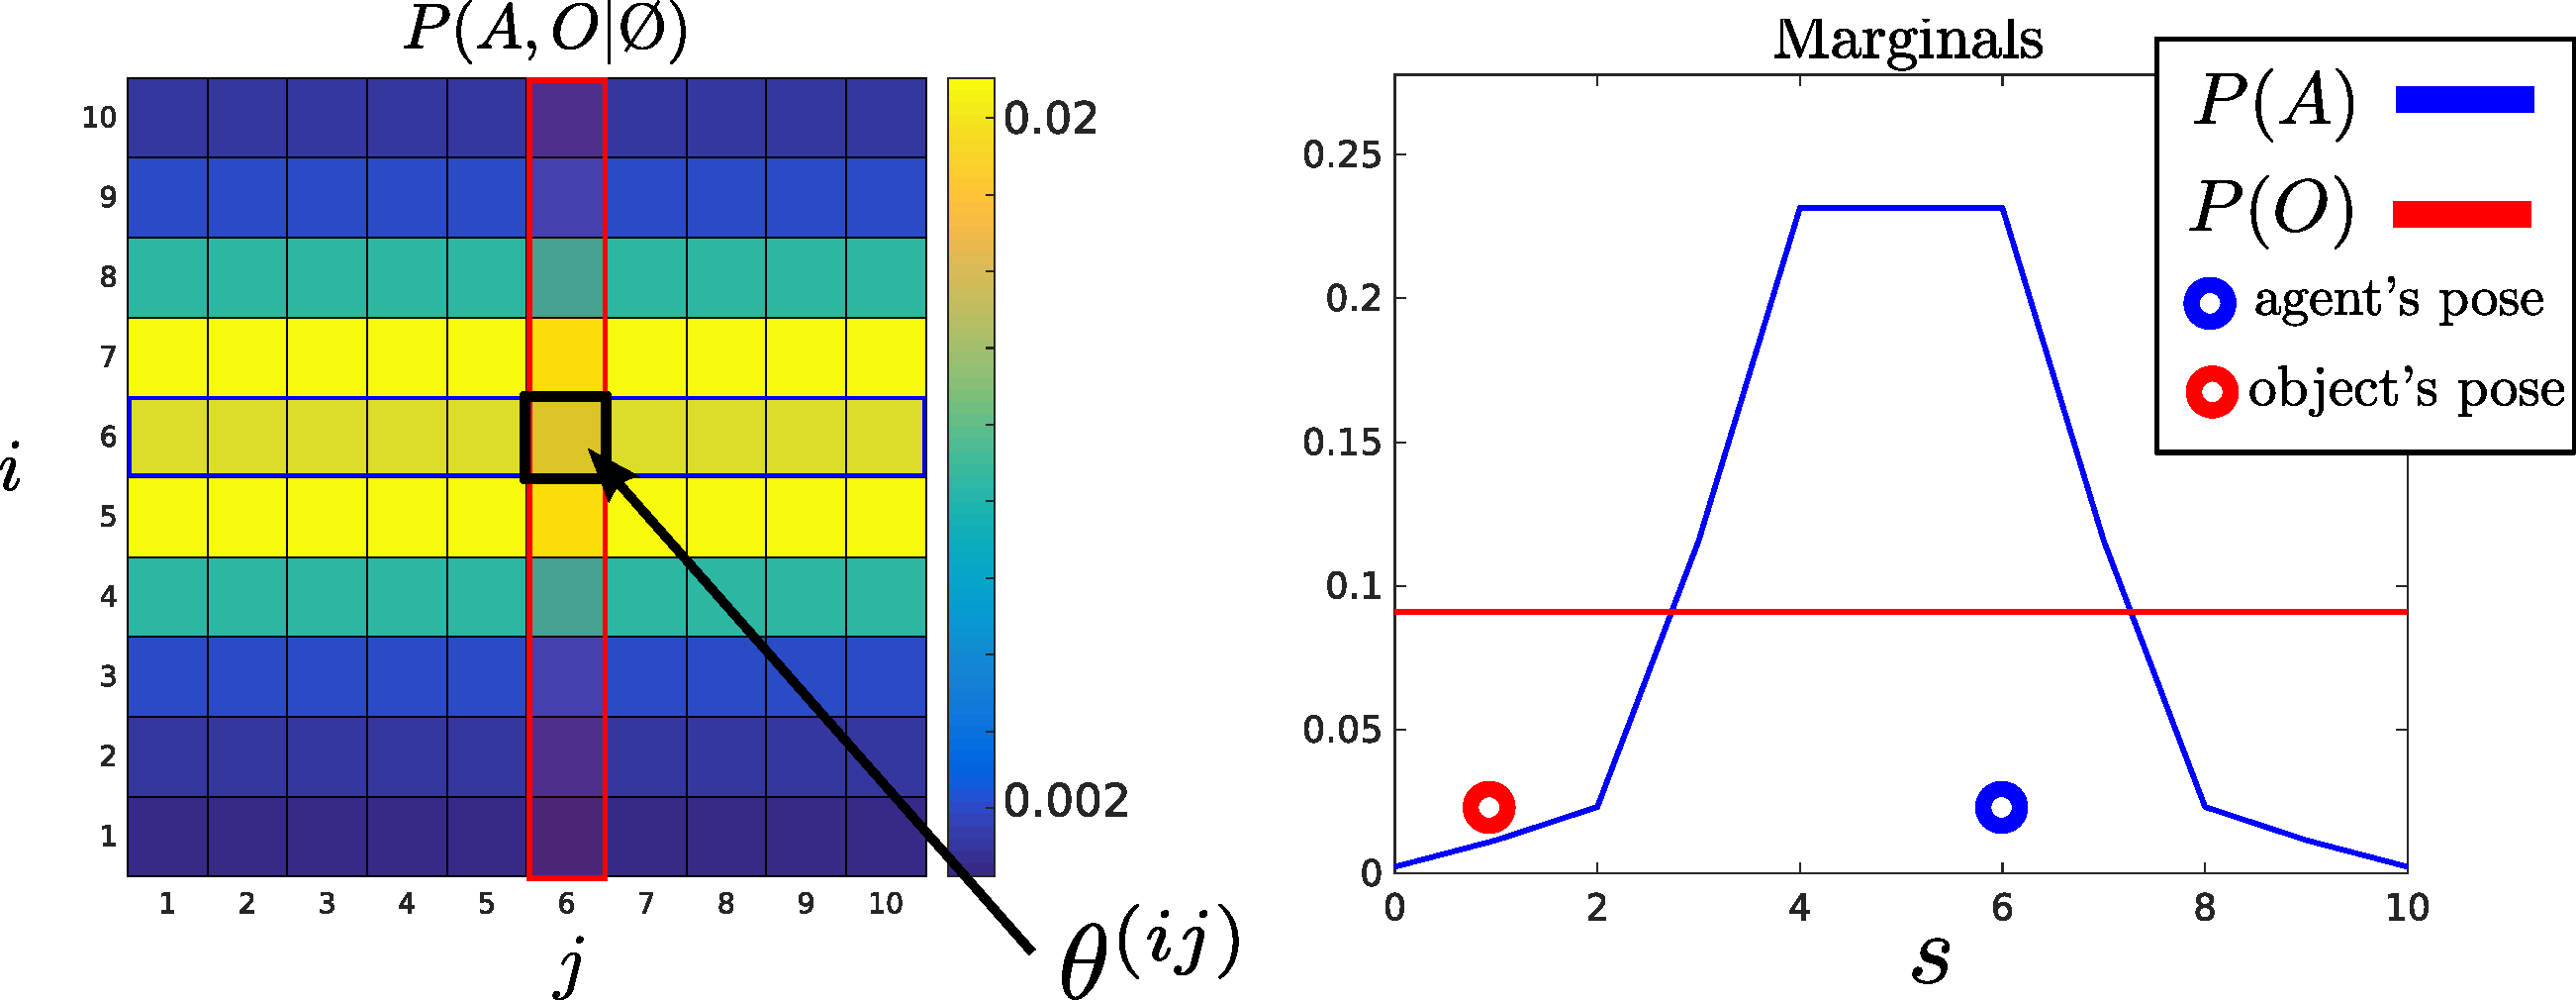
\includegraphics[width=\textwidth]{./ch5-MLMF/Figures/explenation/hist_SLAM.pdf}
 \caption{\textit{Left:} Joint distribution of the agent and object before any action or measurement is integrated. 
 \textit{Right:} Marginals of the agent and object, giving the probability of their location. The marginal of each 
 random variable is obtained from Equation \ref{eq:agent_marginal}. The probability of
 the agent and object begin in state $s=6$ is given by summing the blue and red highlighted parameters in the joint distribution. }
 \label{fig:histogram_joint}
\end{figure}

\paragraph{Histogram likelihood model}

A measurement model, $P(Y_t|A_t,O)$, predicts the likelihood of observations, $Y_t$, given the state of $A_t$ and $O$. 
In the tasks we consider, an observation occurs only if the agent enters in contact with the object, which implies that both
occupy the same discrete state. 
\begin{equation} \label{eq:ch5:discrete_likelihoood}
P(Y_t=1|A_t,O) =
  \begin{cases}
    1       & \quad \text{if } A_t = O     \\
    0  	    & \quad \text{if } A_t \not= O \\
  \end{cases}
\end{equation}

Figure \ref{fig:histogram_likelihood}, illustrates the likelihood of Equation \ref{eq:ch5:discrete_likelihoood} 
in the case when a no contact measurement $Y_t=0$ is present in a 1D world. Both likelihoods are sparse in the sense that there is only a small 
region which gets affected by the likelihood. When there is no measurement (\textit{Left}) all the parameters of the 
joint distribution which are in the black regions will become zero. When the object is detected (\textit{Right}) then 
only parameters of the joint distribution which are within the white regions will be non-zero. All changes
to the joint distribution are constrained to the states $i = j$, which in the case of a 2-dimensional joint 
distribution is a line. The \textbf{sparsity} of the likelihood function  will be key to the development of the MLMF filter.

\begin{figure}
 \centering
 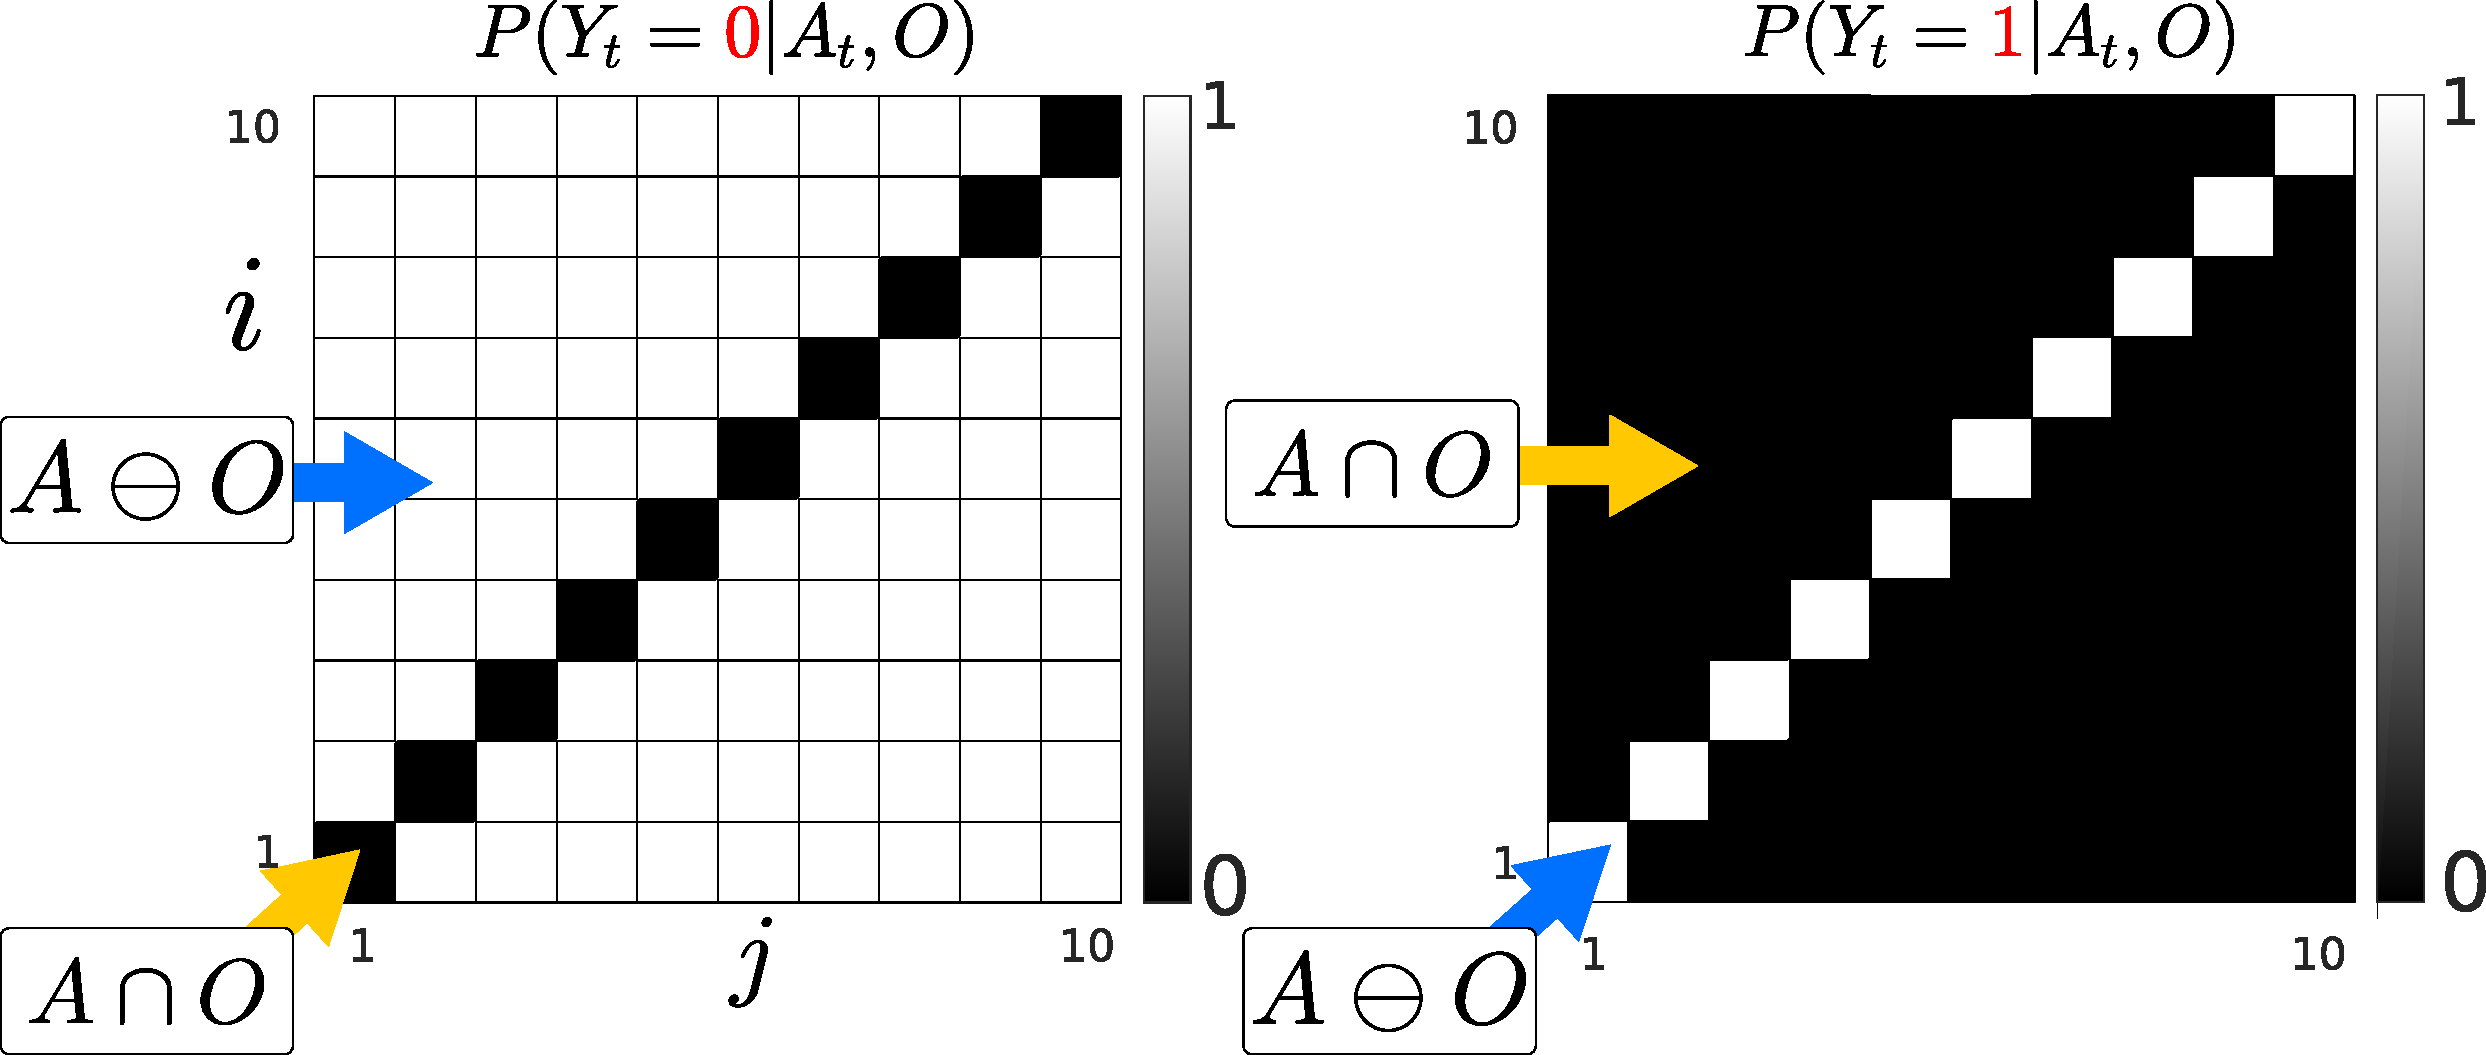
\includegraphics[width=\textwidth]{./ch5-MLMF/Figures/explenation/hist_likelihood.pdf}
 \caption{1D world Likelihood $P(Y_t|A_t,O)$. \textit{Left:} No contact detected with the object, the current measurement 
 is $\hat{Y}_t = \textcolor{red}0$, both the agent and object cannot be in the same state. \textit{Right:} The agent 
 entered into contact with the object and received a haptic feedback $Y_t = \textcolor{red}1$. There are only two measurements 
 contact or no contact, which the agent receives.}
 \label{fig:histogram_likelihood}
\end{figure}

Two models are needed to perform the recursion, namely the motion model $P(A_t|A_{t-1},u_t)$ and the measurement model
$P(Y_t|A_t,O)$, which we already detailed. Both models applied consecutively to the initial joint distribution results in a posterior
distribution. Both Equation \ref{eq:time-update}-\ref{eq:measurement-update} are part of the histogram Bayesian filter 
update:

\begin{center}
\begin{tikzpicture}    
\node [white_box] (box){%
\begin{minipage}{\textwidth}
\vspace*{-1cm}
\begin{align}
 &\mathrm{\textbf{intialisation}}\nonumber\\
 &P(A_0,O) = P(A_0) P(O) = \boldsymbol{\theta}^{(i)} \boldsymbol{\theta}^{(j)} = \boldsymbol{\theta}^{(i,j)} \label{eq:ch5:disc_prod_AO}\\
 &\mathrm{\textbf{motion}}\nonumber\\
 &P(A_t,O|Y_{0:t-1},u_{1:t}) = \sum_{A_{t-1}} P(A_t|A_{t-1},u_t) \cdot  P(A_{t-1},O_t|Y_{0:t-1},u_{1:t-1} \label{eq:ch5:disc_motion})\\
 &\mathrm{\textbf{measurement}}\nonumber\\
 & P(A_t,O|Y_{0:t},u_{1:t}) = \frac{P(Y_t|A_t,O)\cdot P(A_t,O|Y_{0:t-1},u_{t}) }{P(Y_t|Y_{0:t-1})} \label{eq:ch5:disc_measurement} 
\end{align}
\end{minipage}
};
\node[fancytitle, right=10pt] at (box.north west) {Discrete Bayesian filter recursion};
\end{tikzpicture}%
\end{center}

For the derivation of these  two steps, the reader is referred to Appendix \ref{appendix:bayes_recursion}.
Figure \ref{fig:discrete_example} illustrates how the joint distribution evolves in a 1D world. 
The agent and object's true positions (unobservable) are in state 6 and 1. The agent moves four steps towards state 10. At each time 
step, as the agent does not sense the object, the likelihood function  $P(Y_t=0|A_t,O)$ (Figure \ref{fig:histogram_likelihood} \textit{Left})
is applied. As the agent moves towards the right, the motion model shifts the joint distribution towards state 10 along the agent's 
dimension, $i$ (note that state 1 and 10 are wrapped).

\begin{figure}
 \centering
  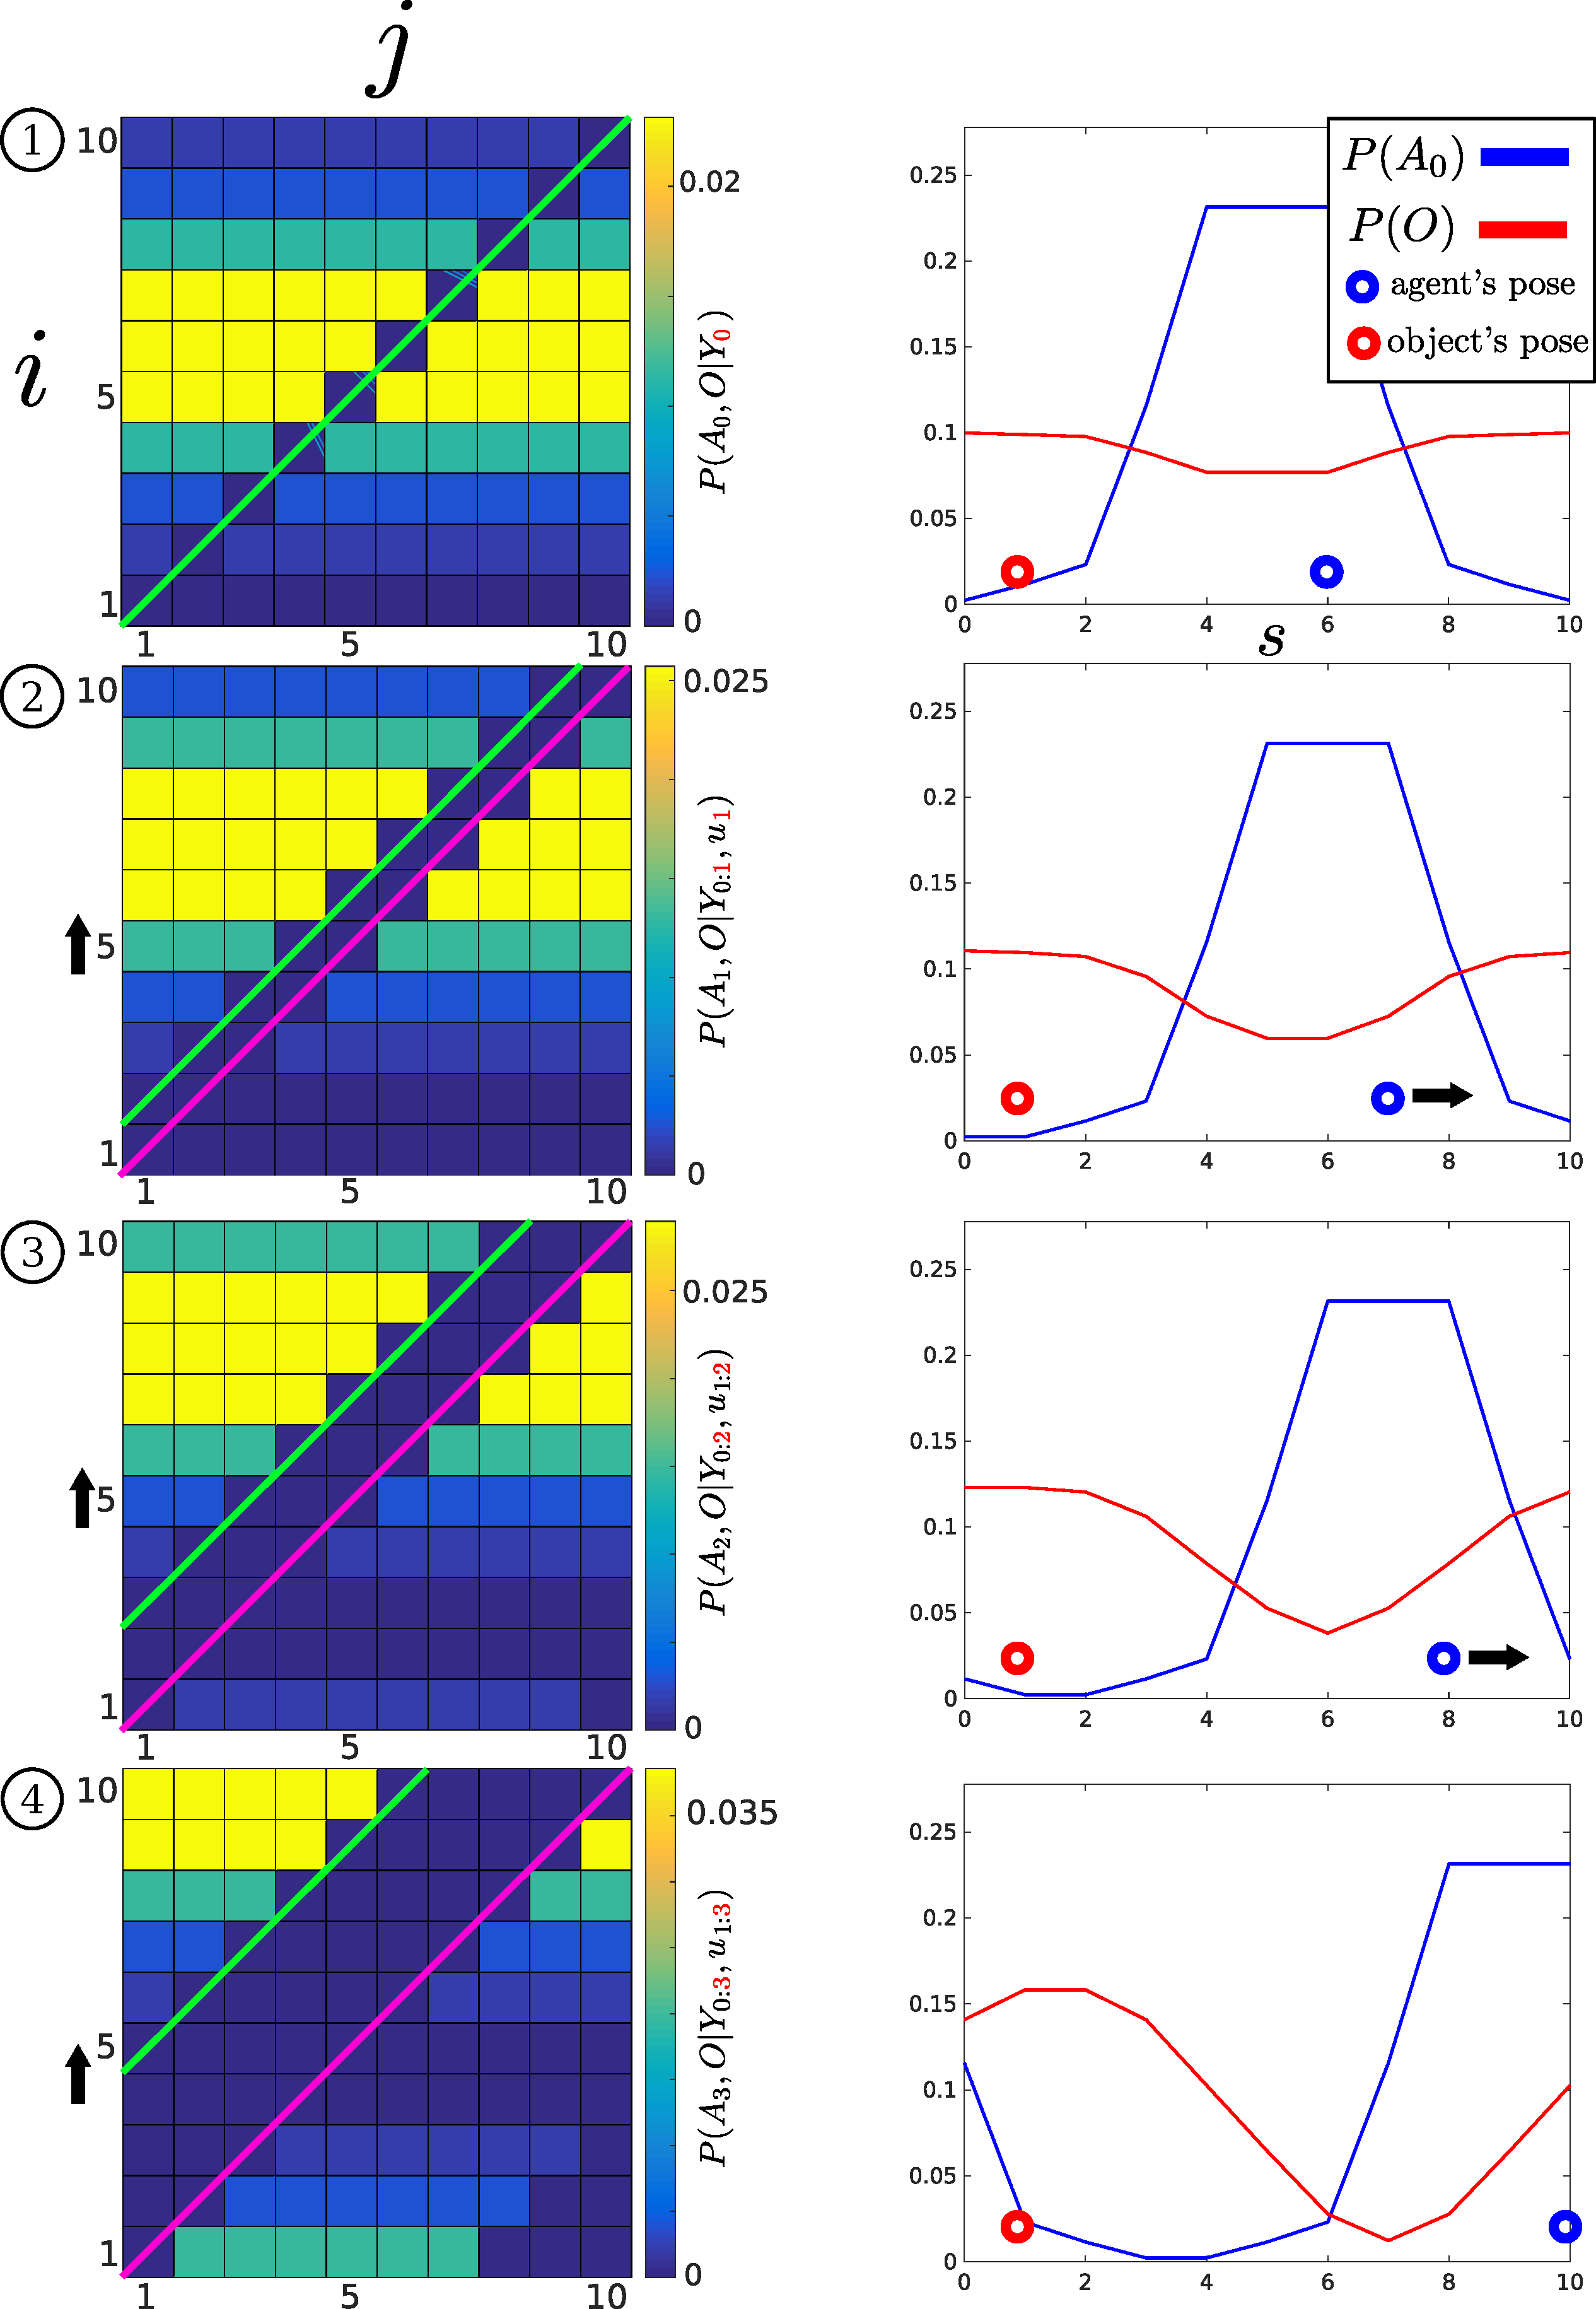
\includegraphics[width=\textwidth]{./ch5-MLMF/Figures/explenation/hist_motion.pdf}
  \caption{Histogram-SLAM, 4 time steps. \textbf{1} Application of likelihood $P(Y_0=0|A_0,O)$ and the agent remains stationary, $u_0=0$, all states along the green line become zero.
  \textbf{2} The agent moves to the right $u_1=1$, the motion $P(A_1|A_0,u_1)$, and likelihood models are applied consecutively. The right motion results in a shift (black arrow on the left) in the joint probability 
  distribution towards the state $i=10$. All parameters on the pink line are zero. \textbf{3} Same as two. \textbf{4} The original result of the likelihood function,
  green line, has moved by the same amount as the agent's displacement. At each time step a new likelihood function (pink line) is applied to the joint distribution.}
  \label{fig:discrete_example}
\end{figure}

As the agent moves to the right more joint distribution parameters become zero and the re-normalisation by the \textbf{evidence} ($P(Y_t|Y_{0:t-1}$, denominator of Equation \ref{eq:ch5:disc_measurement}), 
which increases the value of the remaining parameters, is equal to the sum of the probability mass which was set to zero by the likelihood function.
Thus the values of the parameters of the joint distribution which fall on the pink line in Figure \ref{fig:discrete_example} 
(green line also, but only for first time slice) become zero and their values are redistributed to the remaining non-zero parameters. 
This is an \textbf{important aspect} which will be present in MLMF and we define this to be $\alpha \in \mathbb{R}$.

When the agent enters into contact with the object and senses it, the likelihood function $P(Y_t=1|A_t,O)$, Figure \ref{fig:histogram_likelihood} (\textit{Right}), is 
multiplied with the joint distribution with the result illustrated in Figure \ref{fig:discrete_example_contact}. Only parameters of the joint distribution whose indices
satisfy $i = j$ will remain unchanged, all the others will become zero. In retrospect the likelihood $P(Y_t=1|A_t,O)$ acts as a \textbf{constraint}, 
that is, the agent and object have to be in the same state given by a line traversing the 2D joint distribution.

\begin{figure}
 \centering
 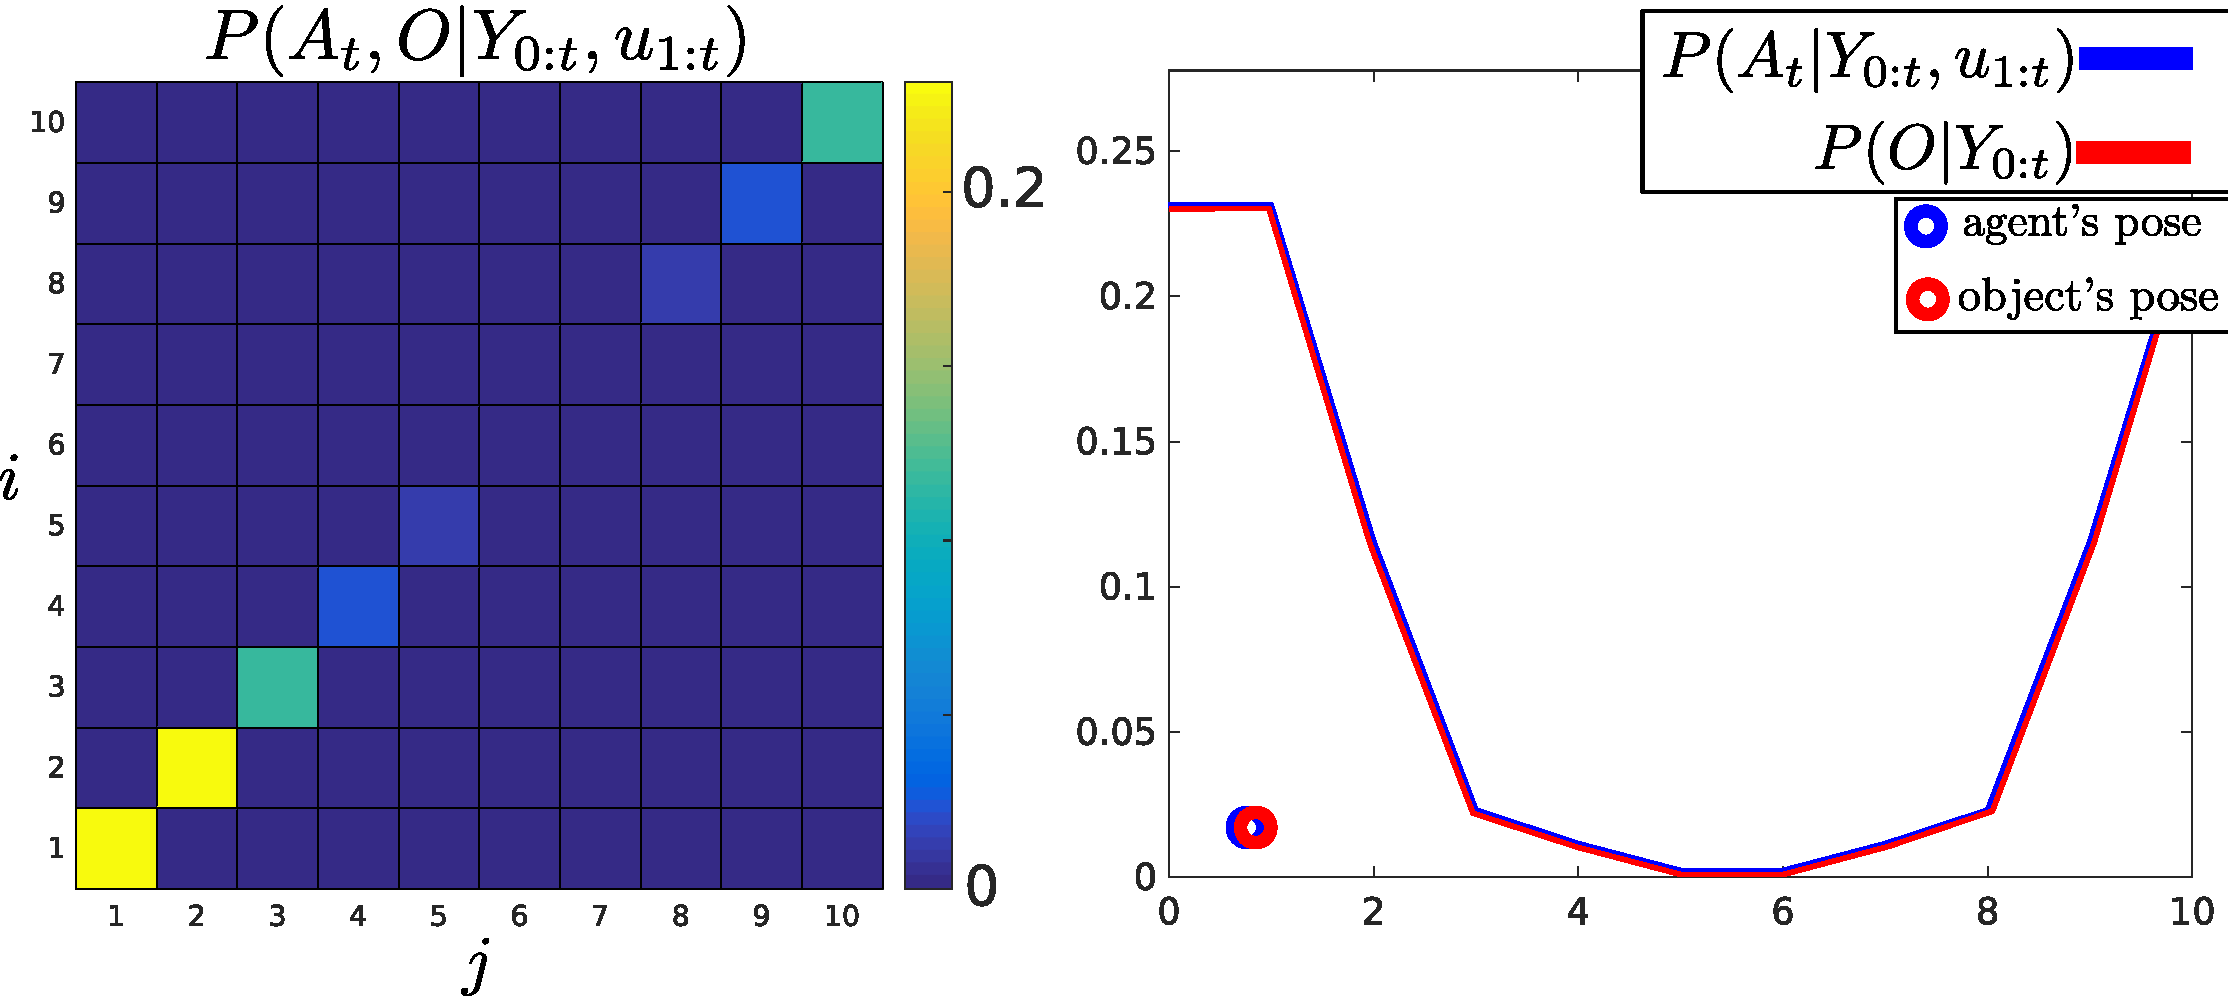
\includegraphics[width=\textwidth]{./ch5-MLMF/Figures/explenation/joint_marginal_contact.pdf}
 \caption{Histogram-SLAM contact. The agent has entered in contact with the object (measurement $Y_t = 1$) and the likelihood function $P(Y_t=1|A_t,O)$ is applied to the joint
 distribution. Only parameters on the line $i=j$ will remain unchanged and parameters for which $i \not= j$ will be set to zero.}
 \label{fig:discrete_example_contact}
\end{figure}

The \textbf{inconvenience} with Histogram-SLAM is that its time and space complexity is exponential, as the joint distribution is discretized and 
parametrised by $\boldsymbol{\theta}^{(ij)}$. Instead we propose a filter, named MLMF, which does not parameterise the joint distribution.

The particularity of the new filter, MLMF, which we formally introduce in the next section, is to achieve the same result as 
the Histogram filter but without having to parameterise the joint distribution, thus avoiding the exponential growth cost. 
The \textbf{key idea} behind the mechanism of the MLMF filter is to only evaluate the joint distribution in states $(i,j)$ 
for which the likelihood is zero and apply the updates directly to the marginals without parameterising the values of the joint distribution.
The MLMF filter parametrises \textbf{explicitly} the marginals $P(A_t=s|Y_{0:t},u_{1:t}): \boldsymbol{\theta}_a^{(s)}$, $P(O=s|Y_{0:t},u_{1:t}): \boldsymbol{\theta}_o^{(s)}$. This is in contrast to the Histogram filter in which the marginals are  
derived from the joint distribution by marginalisation. For the MLMF filter, in order to respect the Bayesian recursion, the filter has 
to \textbf{memorise} the complete history of likelihood functions $\{P(Y_t|A_t,O)\}_{t=0:T}$ and the normalisation coefficient $\alpha$. 
The reasons for this will be made clear in the next section. Below we summarise the parameters of the Histogram and the 
desired MLMF parameters:

\begin{center}
\begin{minipage}{0.55\textwidth}
\fbox{
\begin{tabular}{lcl}
 Histogram    & : & $\boldsymbol{\theta}^{(ij)}$ \\
 desired-MLMF & : & $\boldsymbol{\theta}_a^{(s)}$, $\boldsymbol{\theta}_o^{(s)},\alpha,\{(Y,l)_p\}_{p=0:t}$\\
	      &   & $s,i,j=1,\dots,N$
\end{tabular}
}
\end{minipage}
\end{center}

The likelihood function is parametrised by a measurement, $Y_t$ and offset $l$ to the $i$-axis. In Figure \ref{fig:discrete_example} we see that
the likelihood applied at the first time step (green line) is superimposed on the line $i=j$. As actions are applied, $u_{1:3}=[1,1,1,1]$, 
the first likelihood function (green line) shifts by an amount corresponding to the total displacement (4 in this case), see the last sub-figure of
\ref{fig:discrete_example}. The second likelihood applied at $t=1$ will have an offset corresponding to the sum $u_{1:3}$, the third will have 
an offset of $u_{2:3}$ and so on and so forth.

The MLMF, which we mathematically derive in the next section, keeps as parameters the marginals, likelihood function parameters and a normalisation 
constant. The marginals are updated (filter recursion) by \textbf{evaluating} the joint distribution in states which are set to zero by the current 
applied likelihood and removing the value of the zeroed parameters from the marginals. 

When a positive contact is established with the object, the likelihood is zero everywhere other than the states corresponding to  $i=j$, 
see Figure \ref{fig:discrete_example_contact}. In this case there is no need to evaluate the likelihood elsewhere
in the joint distribution. The marginals are simply the normalisation of the line $i=j$. The evaluation of the joint distribution, 
given that the object is sensed or not, is restricted to the states $(i,j)$ for which $i=j$ and there are a total of $N$ states. 
This is much less than $N^2$ which Histogram-SLAM requires.


\FloatBarrier
\section{Measurement Likelihood Memory Filter}\label{ch5:MLMF}

To obtain an informative update of the marginals, the random variables $A$ and $O$ must remain 
dependent in the absence of a positive observation $Y$. Additionally, this dependence should be efficiently encoded in contrast to the
histogram parametrisation shown in Section \ref{sec:Discrete}. 

The likelihood function $P(Y_t|A_t,O)$ is the cause of the dependence between the random variables. If both the agent and object 
were completely independent, no additional parameters would be required to represent the joint distribution other than the marginals 
$P(A_t)$ and $P(O)$ giving a total of $N M$ parameters (where $N$ is the number of states and $M$ is the number of random variables). 
At the other extreme if every single point in the domain of the random variables was dependent this would require the totality 
of $N^M$ parameters as previously stated in the case of the histogram filter. We propose a method in which we do not model the joint
distribution explicitly but rather only compute its impact on the marginals. 

\subsection{MLMF parametrisation}

%However
%we do not take a recursive approach but rather remember all measurement functions which have been applied since 
%the start. %We start from the definition of the joint distribution Equation \ref{eq:bn_joint_memory} given by BN, which is the starting point to all BSSE.
%\begin{align}
% P(A_{0:t},O,Y_{0:t},u_{1:t}) &= P(A_0)P(O)\prod_{t=0}^{t} \overbrace{P(A_t|A_{t-1},u_{t})}^{=1}  \underbrace{ P(Y_t|A_t,O) }_{\mathrm{memory}} \label{eq:bn_joint_memory} %\nonumber \\
%			      &= P(A_0)P(O) \underbrace{\prod_{t=0}^{t-1} P(Y_t|A_t,O)}_{\mathrm{memory}} \label{eq:bn_joint_memory}
%\end{align}
%From Equation \ref{eq:bn_joint_memory}, we can derive the formulation of the filtering update, Equation \ref{eq:ch5:motion_update}-\ref{eq:joint_filter_memory}
%(see Appendix \ref{appendix:bayes_joint} for complete derivation).

%\begin{equation}
% P(A_0,O,Y_0) =  P(Y_0|A_0,O) P(A_0) P(O) 
%\end{equation}

%The parametrisation of the MLMF is derived from the Bayesian Network (BN) graphical model, Figure \ref{fig:bayesian_sse_dag}, from 
%which can be derived the Bayes filter recursion  Equation \ref{eq:ch5:motion_update}, (see Appendix \ref{appendix:bayes_joint} for complete derivation). 

The concept behind MLMF is to keep a  \textbf{function parameterisation} of the joint distribution instead of a \textbf{value parameterisation} as it is the case 
for Histogram-SLAM. At initialisation the joint distribution is represented by the product of marginals, Equation \ref{eq:ch5:prod_AO}, which 
would result in the joint distribution illustrated in Figure \ref{fig:histogram_joint}, if it were to be evaluated at all states $(i,j)$
as it is done for Histogram-SLAM, Equation \ref{eq:ch5:disc_prod_AO}. MLMF will only evaluate this product at specific states, only when necessary.
At each time step the motion and measurement update are applied, Equation \ref{eq:ch5:mlmf_motion_update}-\ref{eq:ch5:mlmf_motion_update}.
An important distinction is that these updates are performed on the joint distribution, which is not the case in Histogram-SLAM where 
the updates are done on the conditional, Equation \ref{eq:ch5:disc_motion}-\ref{eq:ch5:disc_measurement}. After applying multiple 
motion and measurement updates the resulting joint distribution is given by Equation \ref{eq:ch5:mlmf_filter_joint}, see Appendix \ref{appendix:recursion_example}
for a step-by-step derivation. The filtered condition, Equation \ref{eq:ch5:mlmf_filter_conditional}, is the result of the normalisation of the 
filtered joint by the marginal likelihood.

%  \label{eq:ch5:disc_prod_AO}
%  \label{eq:ch5:disc_motion}
%  \label{eq:ch5:disc_measurement} 
 
\begin{center}
\begin{tikzpicture}    
\node [white_box] (box){%
\begin{minipage}{\textwidth}
\vspace*{-1cm}
\begin{align}
 &\mathrm{\textbf{intialisation}}\nonumber\\
 &P(A_0,O) = P(A_0) P(O) \label{eq:ch5:prod_AO}\\
 &\mathrm{\textbf{motion}}\nonumber\\
 &P(A_t,O,Y_{0:t-1}|u_{1:t}) = \sum_{A_{t-1}} P(A_t|A_{t-1},u_t) P(A_{t-1},O,Y_{0:t-1}|u_{1:t-1})  \label{eq:ch5:mlmf_motion_update} \\
 &\mathrm{\textbf{measurement}}\nonumber\\
 &P(A_t,O,Y_{0:t}|u_{1:t}) = P(Y_t|A_{t},O) P(A_t,O,Y_{0:t-1}|u_{1:t-1})  \label{eq:ch5:mlmf_measurement_update} \\
 &\mathrm{\textbf{filter (joint)}}\nonumber\\
 &P(A_t,O,Y_{0:t}|u_{1:t}) = P(O) P(A_t|u_{1:t}) \prod_{i=1}^{t}P(Y_i|A_t,O) \label{eq:ch5:mlmf_filter_joint} \\
 &\mathrm{\textbf{filter (conditional)}}\nonumber\\
 &P(A_t,O|Y_{0:t},u_{1:t}) = \frac{P(A_t,O,Y_{0:t}|u_{1:t}) }{P(Y_{0:t}|u_{1:t}) } \label{eq:ch5:mlmf_filter_conditional}
\end{align}
\end{minipage}
};
\node[fancytitle, right=10pt] at (box.north west) {MLMF Bayesian filter};
\end{tikzpicture}%
\end{center}

% (see the motion of the blue pdf in Figure \ref{fig:margina_joint_example})
 
The motion update, Equation \ref{eq:ch5:mlmf_motion_update}, when applied to the joint distribution results in the 
initial marginal $P(A_t)$ and the likelihood functions being moved along the agent's axis. Equation \ref{eq:ch5:mlmf_filter_conditional}, would 
require an expensive evaluation of Equation \ref{eq:ch5:mlmf_filter_joint} 
at each state $(i,j)$ resulting in the evaluation of the likelihood product. We will demonstrate that MLMF only evaluates dependent states $(i,j)$ (states which are affected by the likelihood at the current time step).
The MLFM filter is parameterised by the agent and object marginals $P(A_t|u_{1_:t})$, $P(O)$ and the history of likelihood functions,
Equation \ref{eq:ch5:mlmf_filter_joint}, which is all the likelihood functions since $t=0$ until $t$: 

\begin{equation}
 P(Y_{0:t}|A_t,O;\Psi_t) := \prod_{t=0}^t P(Y_t|A_t,O) \label{eq:memory}
\end{equation}
%  as illustrated in Figure \ref{fig:discrete_example} and \ref{fig:margina_joint_example}.
The likelihood functions have two different functional forms (see Figure \ref{fig:histogram_likelihood}) which is dictated 
by the current binary measurement and the offset of the likelihood function along the agent's axis. The parameters of Equation \ref{eq:memory}
are all the measurements since the start of the filtering and offsets along the agent's axis, we refer to these parameters
as $\Psi_t = \{(Y,l)_p\}_{p=0:t}$. In Algorithm \ref{alg:memory-motion}, we detail how a measurement and action at 
time step $t$, result in the update of the likelihood functions; this is an implementation of Equation  \ref{eq:ch5:mlmf_motion_update}
for the likelihood product.

\begin{center}
\begin{minipage}{.65\linewidth}

\begin{algorithm}[H]
\label{alg:memory-motion}
\SetKwInOut{Input}{input}
\SetKwInOut{Output}{output}

\Input{$\Psi_{t-1}$, $Y_t$, $u_t$}
\Output{$\Psi_t$}
\BlankLine
\textbf{motion update}\label{alg:ch5:motion_memory}\\
\For{$l_{t-1} \in \Psi_{t-1}$}{$l_t = update\_offset(l_{t-1},u_t)$}
\textbf{measurement update}\\
$\Psi_t \gets \{\Psi_{t-1}, (Y_t,l=0)\}$ 

\caption{Likelihood motion update}

\end{algorithm} 
\end{minipage}
\end{center}



Figure \ref{fig:margina_joint_example} illustrates the evolution of the MLMF joint distribution, Equation \ref{eq:ch5:mlmf_filter_conditional}, for 
two actions and three measurements. On the \textit{left} a green line passes through the probability mass of the joint distribution which was initialised to $P(A_0,O) = P(A_0) P(O)$. 
The states $(i,j)$ in the joint distribution on the green line are evaluated to zero by the likelihood function $P(Y_0=0|A_t,O)$, since no object was sensed.
As the agent takes two actions towards state 100 the original marginal distribution of the agent, $P(A_0)$, is updated according to Equation \ref{eq:ch5:mlmf_motion_update} as are the 
likelihood functions, resulting in $P(A_2|u_{1:2})$, $P(Y_0|A_2,O)$ and $P(Y_1|A_2,O)$. The likelihood function $P(Y_0|A_2,O)$ evaluates all states $(i+2=j)$ to zero and 
the likelihood $P(Y_1|A_2,O)$ evaluates states $(i+1=j)$ to zero.
A new measurement is sensed and the corresponding likelihood function
$P(Y_2|A_2,O)$ is added to the product of likelihoods, Equation \ref{eq:ch5:mlmf_measurement_update}, which evaluates all states $(i,j)$ to zero.
The parameters of Equation \ref{eq:memory} will now be: $\Psi_2 = \{(0,2)_{p=0},(0,1)_{p=1},(0,0)_{p=2}\}$. 
The probability mass which has been evaluated to zero is re-normalised to the remaining non-zero parameters of the joint distribution, 
as the joint distribution must sum to one.

\begin{figure}
 \centering
 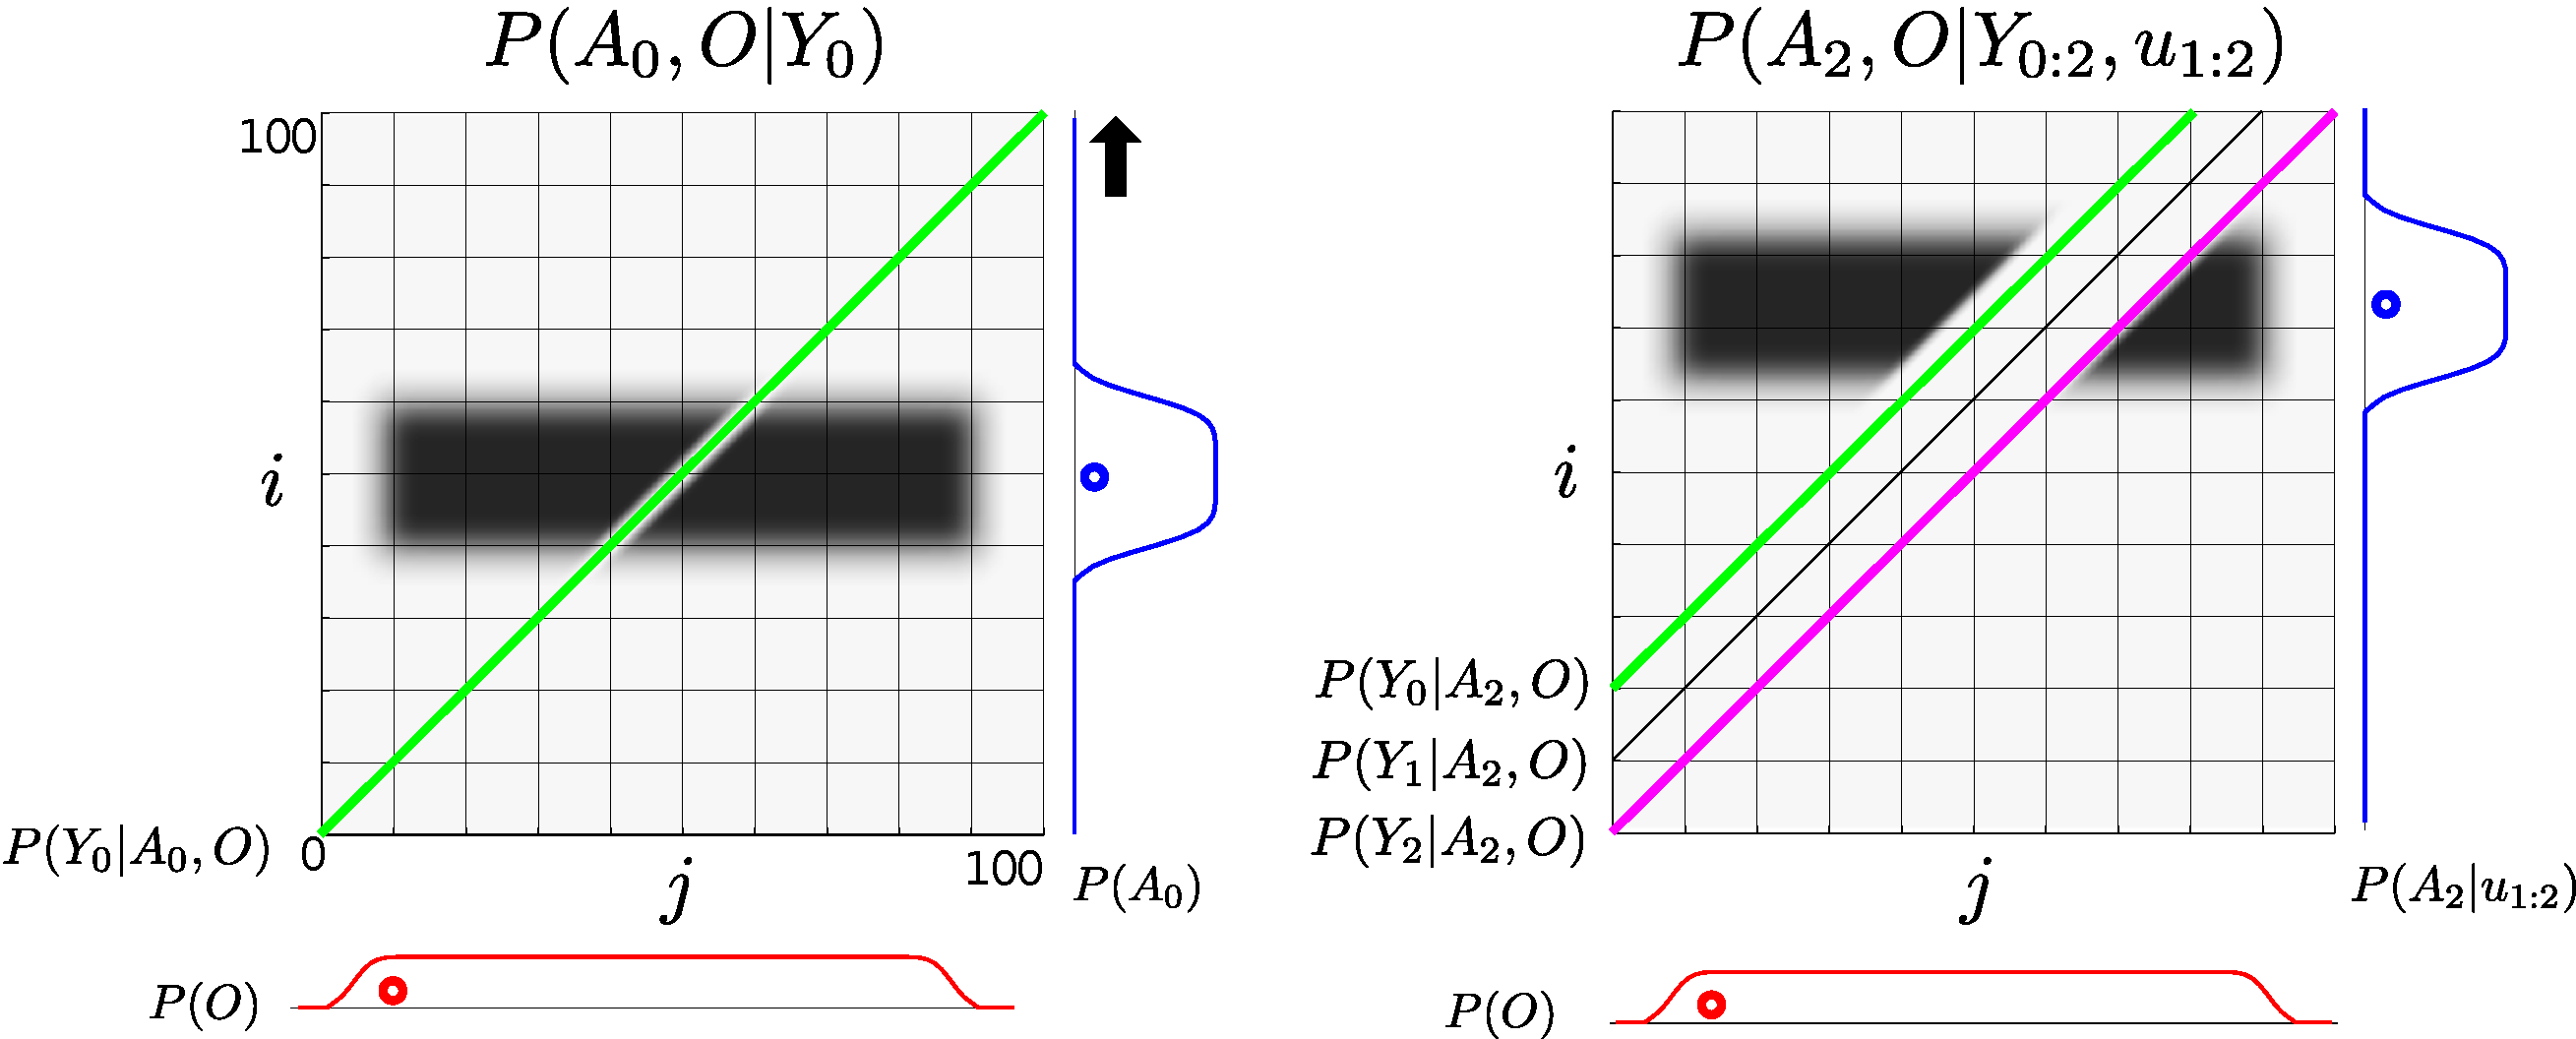
\includegraphics[width=\textwidth]{./ch5-MLMF/Figures/Figure6_v2.pdf}
 \caption{Evolution of the MLMF joint distribution (evaluation of Equation \ref{eq:ch5:mlmf_filter_conditional}) and marginals for a 1D world. The space is discretised to 100 bins and the agent is moving in the direction of the black arrow. 
 The black line correspond to areas in which the likelihood function evaluates to zero.  \textit{Left}: the first 
 likelihood function $P(Y_0|A_0,O)$, causes all the mass of joint distribution whose's states are $i=j$ to be evaluated to zero, as
 the agent has not sensed the object (the red and blue circles on the marginals indicate the true position of
 both the agent and the object). The probability mass which lies in the area of influence of the measurement likelihood (evaluated to zero) gets 
 removed and redistributed to the other states in the joint distribution due to normalisation.
 \textit{Right:} Two actions have be taken and three measurements have been observed. The joint distribution on the \textit{right} is the result of 
 applying the motion update, Equation \ref{eq:ch5:mlmf_motion_update}, which moves the initial marginal $P(A_0)$ to $P(A_2|u_{1:2})$ and displaces the 
 likelihood function. A new measurement is then added, Equation \ref{eq:ch5:mlmf_filter_joint}, illustrated by the pink line.}
 \label{fig:margina_joint_example}
\end{figure}


%which have been applied 
%since initialisation up to the current time step. At every time step the likelihood function get updated by the current action Equation, \ref{eq:ch5:motion_update}.
%The motion update consists of applying the forward dynamics $P(A_t|A_{t-1},u_t)$ to 
%$P(A_{t-1},O|Y_{0:t-1},u_{1:t-1})$ (Equation \ref{eq:bn_joint_memory}) to achieve $P(A_t,O|Y_{0:t-1},u_{1:t})$, see Equation \ref{eq:time_update_memory}. 
%\begin{align}\label{eq:time_update_memory}
% P(A_t,O|Y_{0:t-1},u_{1:t}) &= \sum\limits_{A_{t-1}} P(A_t|A_{t-1},u_t) \cdot  P(A_{t-1},O|Y_{0:t-1},u_{1:t-1})
%\end{align}

%At every time step, the parameters of a new likelihood function, $P(Y_t|A_t,O)$, are added to Equation \ref{eq:memory}.
%The motion update acts on the offset parameters $l$ of the memory function which results in the likelihood functions being shifted
%along the $i$-axis as shown in Figures \ref{fig:discrete_example} and \ref{fig:margina_joint_example} and on the agent's original marginal $P(A_0)$.

%The intuition of these two updates is as follows. At the first time step (after initialisation) we add the first measurement 
%likelihood function which results in the line shown in Figure \ref{fig:margina_joint_example} \textit{left}; $\Psi_0 = \{(Y_0=0,u_0=0)\}$. 
%A motion update is applied and the likelihood function shifts along the agent's $i$-axis by the displacement caused by the forward motion and a new 
%likelihood function is added with no offset resulting in a new line $i=j$ in the joint distribution, 
%which is the result of the current measurement after the motion update. Repeating this process results in the white band present 
%in Figure \ref{fig:margina_joint_example} \textit{right}. 

For ease of notation from this point onwards we will not show the conditioned actions $u_{1:t}$, so $P(A_t,O|Y_{0:t},u_{1:t})$ will 
be $P(A_t,O|Y_{0:t})$.

Our goal is to be able to compute the marginals $P(A_t|Y_{0:t})$, $P(O|Y_{0:t})$ of the agent and object random variables and 
marginal likelihood $P(Y_{0:t}|u_{1:t})$ \textbf{without} having to perform an \textbf{expensive marginalisation} over the entire space of the joint distribution 
as was the case for Histogram-SLAM. 

The next section describes how to efficiently compute the normalisation factor, denominator Equation \ref{eq:ch5:mlmf_filter_conditional}, and the marginals.


\subsection{Computation of evidence and marginals}

In order to compute efficiently the marginal likelihood (also known as evidence) $P(Y_{0:t}|u_{1:t})$ and the filtered  marginals $P(A_t|Y_{0:t})$,
$P(O|Y_{0:t})$ we take advantage of the fact that only a very small area 
in the joint distribution space will be affected by the measurement likelihood function at each time step.

Without lost of generality the likelihood function will only make a difference to dependent $A \cap O$ regions in the joint distribution, areas 
where the likelihood function is less than one. The region inside $A \ominus O$ will not be affected, where the likelihood function 
is equal to one.
Figure \ref{fig:overlap_dependence_independence} shows the relation between the measurement 
function $P(Y_t|A_t,O)$ and the joint distribution $P(A_t,O|Y_{0:t})$ for three different initialisations. 

%effect on the joint distribution for three different initialisations. 
%
%  The tube's boundary is governed by the bandwidth of the radial basis function of the likelihood function.
%  Any probability mass of the joint  distribution which lies in the tube will be in the $\cap$, all probability 
%  mass outside the tube but still within the grey rectangle is located in $\ominus$ and 
%  the white space is in the domain but not parametrised and thus not considered.
 
 \begin{figure}
 \centering
  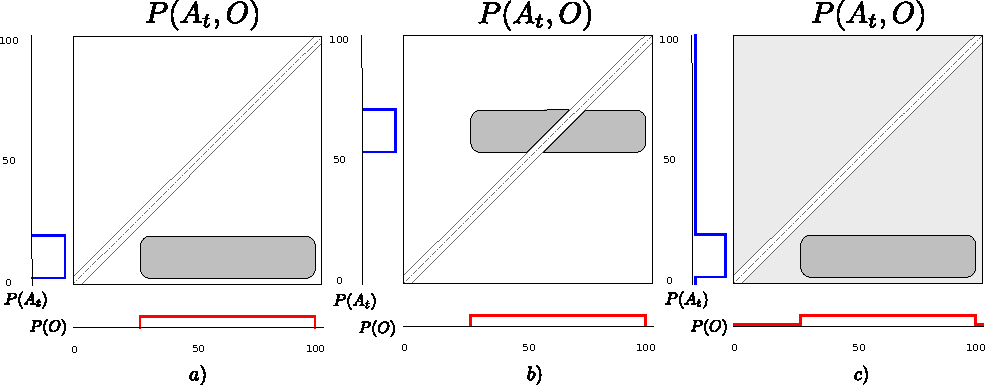
\includegraphics[width=\textwidth]{./ch5-MLMF/Figures/Figure7.pdf}
  \caption{
  \textbf{a)} Likelihood $P(Y_t=0|A_t,O)$, the blue area depicts the regions in which the likelihood is $<1$ 
  and the red area is where the likelihood is $=1$. If the probability mass of the joint distribution 
  is in the blue region, then the parameters of the random variables in these areas are dependent, $A \cap O$
  and otherwise they are independent from one another, $A \ominus O$.  
   \textbf{b)} The agent and object marginals are not overlapping and thus are completely independent. The joint distribution, 
   $P(A_t,O|Y_{0:t})$ the black rectangle,  is not intersecting with the measurement function. As a result $P_{\cap}(A_t,O|Y_{0:t})$
   is empty.
 \textbf{c)} The marginals overlap resulting in the measurement likelihood function intersecting with the joint distribution.
 The joint distribution is composed of the blue and red areas, Equation \ref{eq:joint_independent_dependent}.
 The probability mass at the intersection gets removed and re-normalised to other regions which is the result of applying Bayes integration. 
 \textbf{d)} The marginals of $A$ and $O$ are completely overlapping, however only a small fraction of the probability mass 
 in the joint distribution is within the measurement function's tube.}
  \label{fig:overlap_dependence_independence}
\end{figure}
%\end{FPfigure}

As illustrated and explained in Figure \ref{fig:overlap_dependence_independence}, the joint distribution can be decomposed in a 
dependent and independent term (Equation \ref{eq:joint_independent_dependent}). 

\begin{equation}\label{eq:joint_independent_dependent}
 P(A_t,O|Y_{0:t}) = P_{\cap}(A_t,O|Y_{0:t}) + P_{\ominus}(A_t,O|Y_{0:t})
\end{equation}

The probability mass covered by the dependent term is located within the measurement function's tube and the independent probability mass 
is located outside as shown in Figure \ref{fig:overlap_dependence_independence}. This formulation will lead to large computational gain 
as the independent term is not influenced by the measurement function: 
$P_{\ominus}(A_t,O|\mathbf{Y_{0:t}}) \propto P_{\ominus}(A_t,O|\mathbf{Y_{0:t-1}})$.

\paragraph{Evidence}\\
The evidence of the measurement $P(Y_{0:t}|u_{1:t})$ is the normalisation coefficient of the joint distribution Equation \ref{eq:ch5:mlmf_filter_conditional}.
It is the amount of probability mass re-normalised to the other parameters as a result of the consecutive application of the likelihood function.
At time step $t$, the normalising factor to be added to the evidence is the difference between the probability mass located 
inside $A\cap O$ before and after the application of the measurement function $P(Y_t|A_t,O)$, 
see Equation \ref{eq:I} (see Appendix \ref{appendix:evidence} for the full derivation).

\begin{align}\label{eq:I}
 &P(Y_0)          		= 1 + \sum\limits_{A_0}\sum\limits_{O} P(Y_0|A_0,O)P_{\cap}(A_0,O) - P_{\cap}(A_0,O) \\
 &\alpha_0 			= \sum\limits_{A_0}\sum\limits_{O} P(Y_0|A_0,O)P_{\cap}(A_0,O) - P_{\cap}(A_0,O)\\
 &\alpha_t 	  		= \alpha_{t-1} + \sum\limits_{A_t}\sum\limits_{O} (1 - P(Y_t|A_t,O)) P_{\cap}(A_t,O|Y_{0:t-1}) \\
 &P(Y_{0:t}|u_{1:t})      	= 1 - \alpha_{t}
\end{align}
The advantage of Equation \ref{eq:I} is that the summation is only over states which are in the dependent area $\cap$ of the joint 
distribution. This is generally always much smaller than the full space itself.
Until an object is sensed, the likelihood will always be zero $P(Y_t|A_t,O) = 0$ and $\alpha$ will correspond to the probability 
mass which falls within the region of the joint distribution in which the likelihood function is zero. In Figure 
\ref{fig:overlap_dependence_independence} b) \& d), the sum of the probability mass in the blue 
regions is equal to $\alpha$.
The point of interest is that as we perform the filtering process we will never re-normalise the whole joint distribution, but only keep 
track of how much it should have been normalised. To this end the marginals $P(A_t|u_{1:t})$ and $P(O)$  are never re-normalised but are used 
to compute at each step how much of the probability mass $\alpha_t$ should go to the normalisation factor $P(Y_{0:t}|u_{1:t})$. 
The evidence in question will never be negative, as the joint distribution sums to one and each $\alpha_t$ represents some of the mass removed from the joint distribution. Since we 
keep track of the history of applied  measurement likelihood functions we never remove the same amount of probability mass twice
from the joint distribution.

\paragraph{Marginals}

There are two different types of marginals used in the MLMF filter. The first set are the initial \textbf{joint marginals} of the joint distribution, Equation \ref{eq:ch5:mlmf_filter_joint}.
The second set of marginals are the \textbf{filtered marginals} which are updated by evaluating the joint distribution in dependent states.
%and the filtered marginals, which will derive. The first set of marginals are the initial beliefs and they are part of the parameterisation of the joint distribution, 
%which is only evaluated in dependent states. 


\begin{center}
\begin{tikzpicture}    
\node [white_box] (box){%
\begin{minipage}{0.6\textwidth}
\textbf{joint marignals}\\
$P(A_t|u_{1:t})$ and  $P(O)$: Equation \ref{eq:ch5:mlmf_filter_joint}\\
\textbf{filtered marignals}\\
$P(A_t|Y_{0:t},u_{1:t})$ and $P(O|Y_{0:t})$
\end{minipage}
};
\node[fancytitle, right=10pt] at (box.north west) {Marginals};
\end{tikzpicture}%
\end{center}

%The filtered marginal of the agent and object random variable is acquired by marginalising the joint distribution. 
In Histogram-SLAM both the agent and object marginals are obtained, at every time, by marginalising the joint distribution.
This requires storing and summing over all the parameters of the joint distribution which is expensive.
Instead in MLMF we take advantage of the sparsity of the likelihood function and as a result we take only the dependent marginal components into consideration, 
Equation \ref{eq:marignal_mrf}. 
%\begin{align}
%  &P(A_t|Y_{0:t},u_{1:t}) = \sum\limits_{O}   P(A_t,O|Y_{0:t},u_{1:t}) = \overbrace{\sum\limits_{O} P_{\cap}(A_t,O|Y_{0:t},u_{1:t})}^{P_{\cap}(A_t|Y_{0:t},u_{1:t})} + \overbrace{\sum\limits_{O} P_{\ominus}(A_t,O|Y_{0:t},u_{1:t})}^{P_{\ominus}(A_t|Y_{0:t},u_{1:t})}   \nonumber \\
%  &P(O|Y_{0:t})   = \sum\limits_{A_t} P(A_t,O|Y_{0:t},u_{1:t}) = \sum\limits_{A_t} P_{\cap}(A_t,O|Y_{0:t},u_{1:t}) + \sum\limits_{A_t} P_{\ominus}(A_t,O|Y_{0:t},u_{1:t})\nonumber
%\end{align}
%In MLMF, in contrast to Histogram-SLAM, we only parameterise
%the marginals (not the full joint distribution) and update them where measurements have an effect,  Equation \ref{eq:marignal_mrf} (we dropped $u_{1:t}$ for 
%easing the notation)
%As for the evidence, the marginal is evaluated only in areas of the joint distribution which are dependent and uses the previously 
%computed evidence to normalise this region of the joint distribution during the marginalisation process, Equation \ref{eq:marignal_mrf}

\begin{equation}
 P(A_t|Y_{0:t})  =  P(A_t|Y_{0:t-1}) - \Big(P_{\cap}(A_t|Y_{0:t-1}) -  \mathbf{P_{\cap}(A_t|Y_{0:t}})  \Big) \label{eq:marignal_mrf} 
\end{equation}
(see Appendix \ref{appendix:marginal} for the full derivation of Equation \ref{eq:marignal_mrf}).

\begin{align}\label{eq:marignal_mrf_2}
 \mathbf{P_{\cap}(A_t|Y_{0:t})} &= \frac{ \sum\limits_{O} \overbrace{ P(Y_t|A_{t},O) P_{\cap}(A_t,O,Y_{0:t-1}|u_{1:t})  }^{P_{\cap}(A_t,O,Y_{0:t}|u_{1:t})}}{\underbrace{1  - (\alpha_{0} + \alpha_{1} + \cdots + \alpha_{t})}_{P(Y_{0:t}|u_{1:t})}} \\
		       &= \sum\limits_{O} P_{\cap}(A_t,O|Y_{0:t})
\end{align}

\begin{figure}
\centering
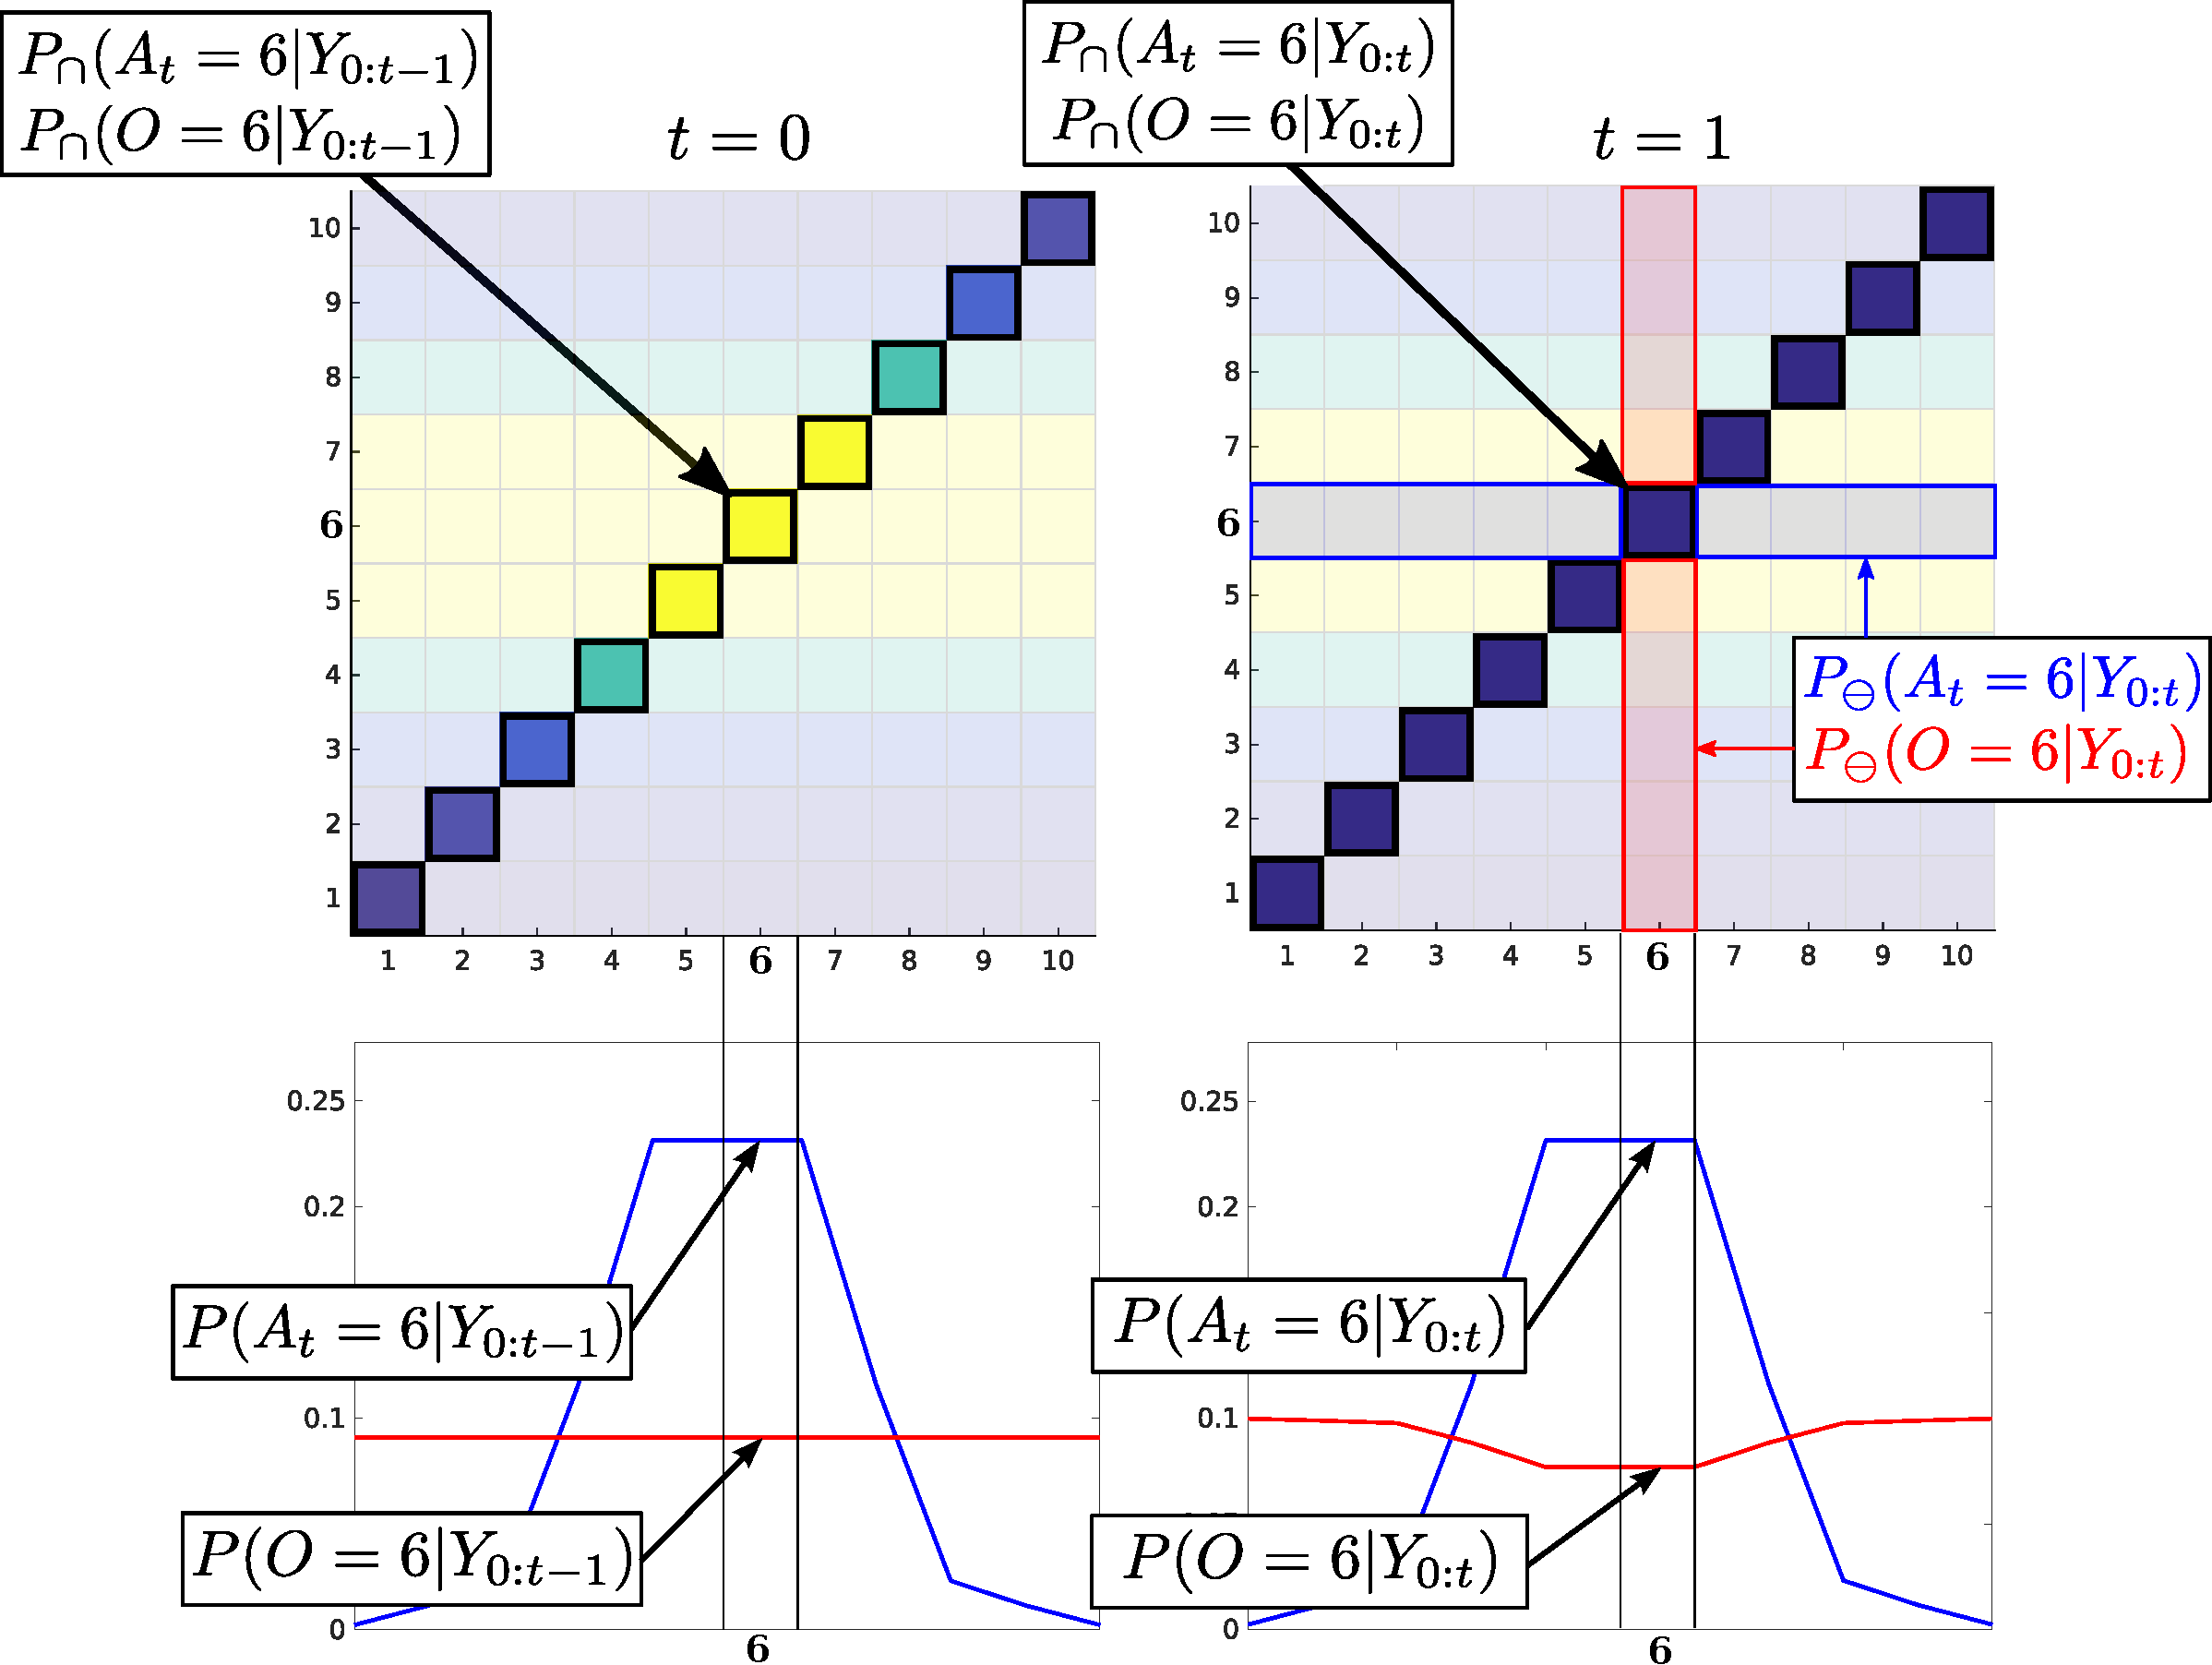
\includegraphics[width=0.95\textwidth]{./ch5-MLMF/Figures/explenation/marginal_cal_example.pdf}
\caption{Filtered Marginals. Illustration of the agent and object marginal update, Equation \ref{eq:marignal_mrf}. The parameters of the joint 
distribution which are independent $A \ominus O$ are pale and the dependent areas $A \cap O$, where $P(Y_t<1|A_t,O)$, are bright. MLMF only
evaluates the joint distribution in dependent states. For each state $s$ of the marginals $1,\dots,10$ the difference 
of the marginals inside the dependent area, before and after the measurement likelihood is applied, is evaluated and removed from the marginals 
$P(A_t|Y_{0:t-1})$, $P(O|Y_{0:t-1})$ leading to $P(A_t|Y_{0:t})$, $P(O|Y_{0:t})$ (we did not show $u_{1:t}$ for easing the notation). }
\label{fig:ch5:marginal_update}
\end{figure}

Equation \ref{eq:marignal_mrf} is recursive, $P(A_t,|Y_{0:\mathbf{t}})$ is computed in terms of  $P(A_t,|Y_{0:\mathbf{t-1}})$. In 
Figure \ref{fig:ch5:marginal_update} we illustrate how the MLMF updates the marginals of the agent and object given a new measurement.
The illustrated marginals (\textit{Bottom row}) are the \textbf{filtered marginals} $P(A_t|Y_{0:t},u_{1:t})$, $P(O|Y_{0:t})$. The shape of the \textbf{joint marginals} $P(A_t|u_{1:t})$, $P(O)$
(not shown) will remain unchanged by measurements during the filtering process. They are the parameters of the joint distribution used to 
update the filtered marginals.



Table \ref{tab:mlmf_parameters} summarises the functions and parameters of the MLMF for two random variables, an agent and object.
\begin{table}[h]
\centering
\fbox{
\begin{tabular}{lcll}
    functions             	&   & parameters                      & description \\\hline
  $P(A_t|Y_{0:t},u_{1:t})$      & : & $\boldsymbol{\theta}_a$	      & filtered marginals\\
  $P(O|Y_{0:t})$          	& : & $\boldsymbol{\theta}_o$	      &  \\
  $P(A_t|u_{1:t})$       	& : & $\boldsymbol{\theta}^*_a$       & joint marginals\\
  $P(O)$                  	& : & $\boldsymbol{\theta}^*_o$       & \\
  $P(Y_{0:t}|u_{1:t})$      	& : & $\alpha \in \mathbb{R}$         & evidence\\
  $P(Y_{0:t}|A_t,O)$      	& : & $ \Psi = \{(Y,l)_p\}_{p=0:t}$ & likelihood history
\end{tabular}
}
\caption{MLMF functions with associated parameters. The marginal parameters are the discretisation of the 
state space $\boldsymbol{\theta} \in \mathbb{R}^N$, $\boldsymbol{\theta}^{(s)}$ corresponds to the probability being in state $s$.}
\label{tab:mlmf_parameters}
\end{table}

\subsection{MLMF-SLAM Algorithm}

\begin{center}
\begin{minipage}{\linewidth}

\begin{algorithm}[H]
\label{alg:mrf-slam}
\SetKwInOut{Input}{input}
\SetKwInOut{Output}{output}
\Input{\\
       \textbf{measurements}\\
	$Y_t$, $u_t$\\
       \textbf{joint functions}:\\
       $P(A_{t-1}|u_{1:t-1})$ $P(O)$, $P(Y_{0:t-1}|A_{t-1},O)$, $\alpha_{0:t-1}$ \\
       \textbf{filtered marginals}:\\
       $P(A_{t-1}|Y_{0:t-1},u_{1:t-1})$, $P(O|Y_{0:t-1})$}
\Output{\\
       \textbf{joint functions}:\\
        $P(A_t|u_{1:t})$, $P(Y_{0:t}|A_t,O)$, $\alpha_{0:t}$\\
       \textbf{filtered marginals}:\\
	$P(A_t|Y_{0:t},u_{1:t})$, $P(O|Y_{0:t})$}
\BlankLine
\textbf{motion update}\\
$P(A_t|u_{1:t})  = \sum\limits_{A_{t-1}} P(A_t|A_{t-1},u_t) \cdot P(A_{t-1}|u_{1:t-1})$\\
$P(A_t|Y_{0:t-1},u_{1:t})  = \sum\limits_{A_{t-1}} P(A_t|A_{t-1},u_t) \cdot P(A_{t-1}|Y_{0:t-1},u_{1:t-1})$\\
$P(Y_{0:t-1}|A_t,O) \gets$ motion update Algorithm \ref{alg:ch5:motion_memory} 
\BlankLine
\textbf{measurement update}
\BlankLine
$P(A_t|Y_{0:t}) = P(A_t|Y_{0:t-1}) - \Big(P_{\cap}(A_t|Y_{0:t-1}) -  P_{\cap}(A_t|Y_{0:t}) \Big)$  \\
$P(O|Y_{0:t}) = P(O|Y_{0:t-1}) -  \Big(  P_{\cap}(O_t|Y_{0:t-1}) -  P_{\cap}(O_t|Y_{0:t})\Big)$    \\
$\alpha_{0:t} = \alpha_{0:t-1} +  \sum\limits_{A_t}\sum\limits_{O} P_{\cap}(A_t,O|Y_{0:t-1}) (1 - P(Y_t|A_t,O))$ \\

$P(Y_{0:t}|A_{0:t},O) \gets$ measurement update Algorithm \ref{alg:ch5:motion_memory} 
\caption{MLMF-SLAM}
\end{algorithm} 
\end{minipage}
\end{center}
In Algorithm \ref{alg:mrf-slam} we detail the motion-measurement update steps of MLMF-SLAM.
This formulation is advantageous as the joint distribution is only evaluated inside the dependent regions 
$A\cap O$ of the joint distribution. Through the term $P(Y_{0:t}|A_t,O)$ we keep 
track of the normalisation factor $P(Y_t|Y_{0:t-1})$ which 
is a scalar, and where we have previously applied the likelihood function. 

We evaluated this formulation of the joint distribution with the standard histogram filter in the case of the 1D search routine 
illustrated in Figure \ref{fig:margina_joint_example} and we found them to be identical. Having respected the formulation of Bayes rule, we
assert that Algorithm \ref{alg:mrf-slam} is a Bayesian Optimal Filter.
\footnote{An optimal Bayesian solution is an exact solution to the recursive problem of calculating the exact posterior density 
\cite{PF_tutorial_2002}}.

\subsection{Space \& time complexity}\label{ch5:space_time_complexity_MLMF}

For discussion purposes we consider the case of three beliefs, namely that of the agent and two other objects $O^{(1)}$ and $O^{(2)}$ which we
subsequently generalise. As stated previously $M$ stands for the number of filtered random variables including the agent. 
$N$ is the number of discrete states in the world. In the following section, we compare MLMF-SLAM with the Histogram-SLAM.

%At every time step we store the action, $u_t \in D$, only if the current marginals have changed as a result of the measurement likelihood function, $P(Y_t|A_t,O)$.


\subsubsection{Space complexity}

Figure \ref{fig:3bel_lik_profile} \textit{left} illustrates the volume occupied by the joint distribution for a marginal space of $N$ states. 
Histogram-SLAM would require $N^3$ parameters for the joint distribution $P(A,O^{(1)},O^{(2)})$ and $N^{M}$ for $M$ random variables. 

For MLMF-SLAM, each random variable $X$ requires two sets parameters $\boldsymbol{\theta}$ and $\boldsymbol{\theta}^*$ 
(see Table \ref{tab:mlmf_parameters}). Given
$M$ random variables, the initial number of parameters is $M \cdot (2 \cdot N)$.
At every time step the likelihood memory function increments by one measurement and offset, $(Y_t,l=0)$ (Algorithm \ref{alg:ch5:motion_memory}).
Given a state space of size $N$, there can be no more than $N$ different measurement functions (one for each state). In
the worst case scenario the space complexity of the memory will be $N$, giving a total of $M \cdot (2 \cdot N) + N$. 
The final worst case space complexity is linear in the number of random variables, $\BigO(N\,M)$. 

\begin{figure}
 \centering
  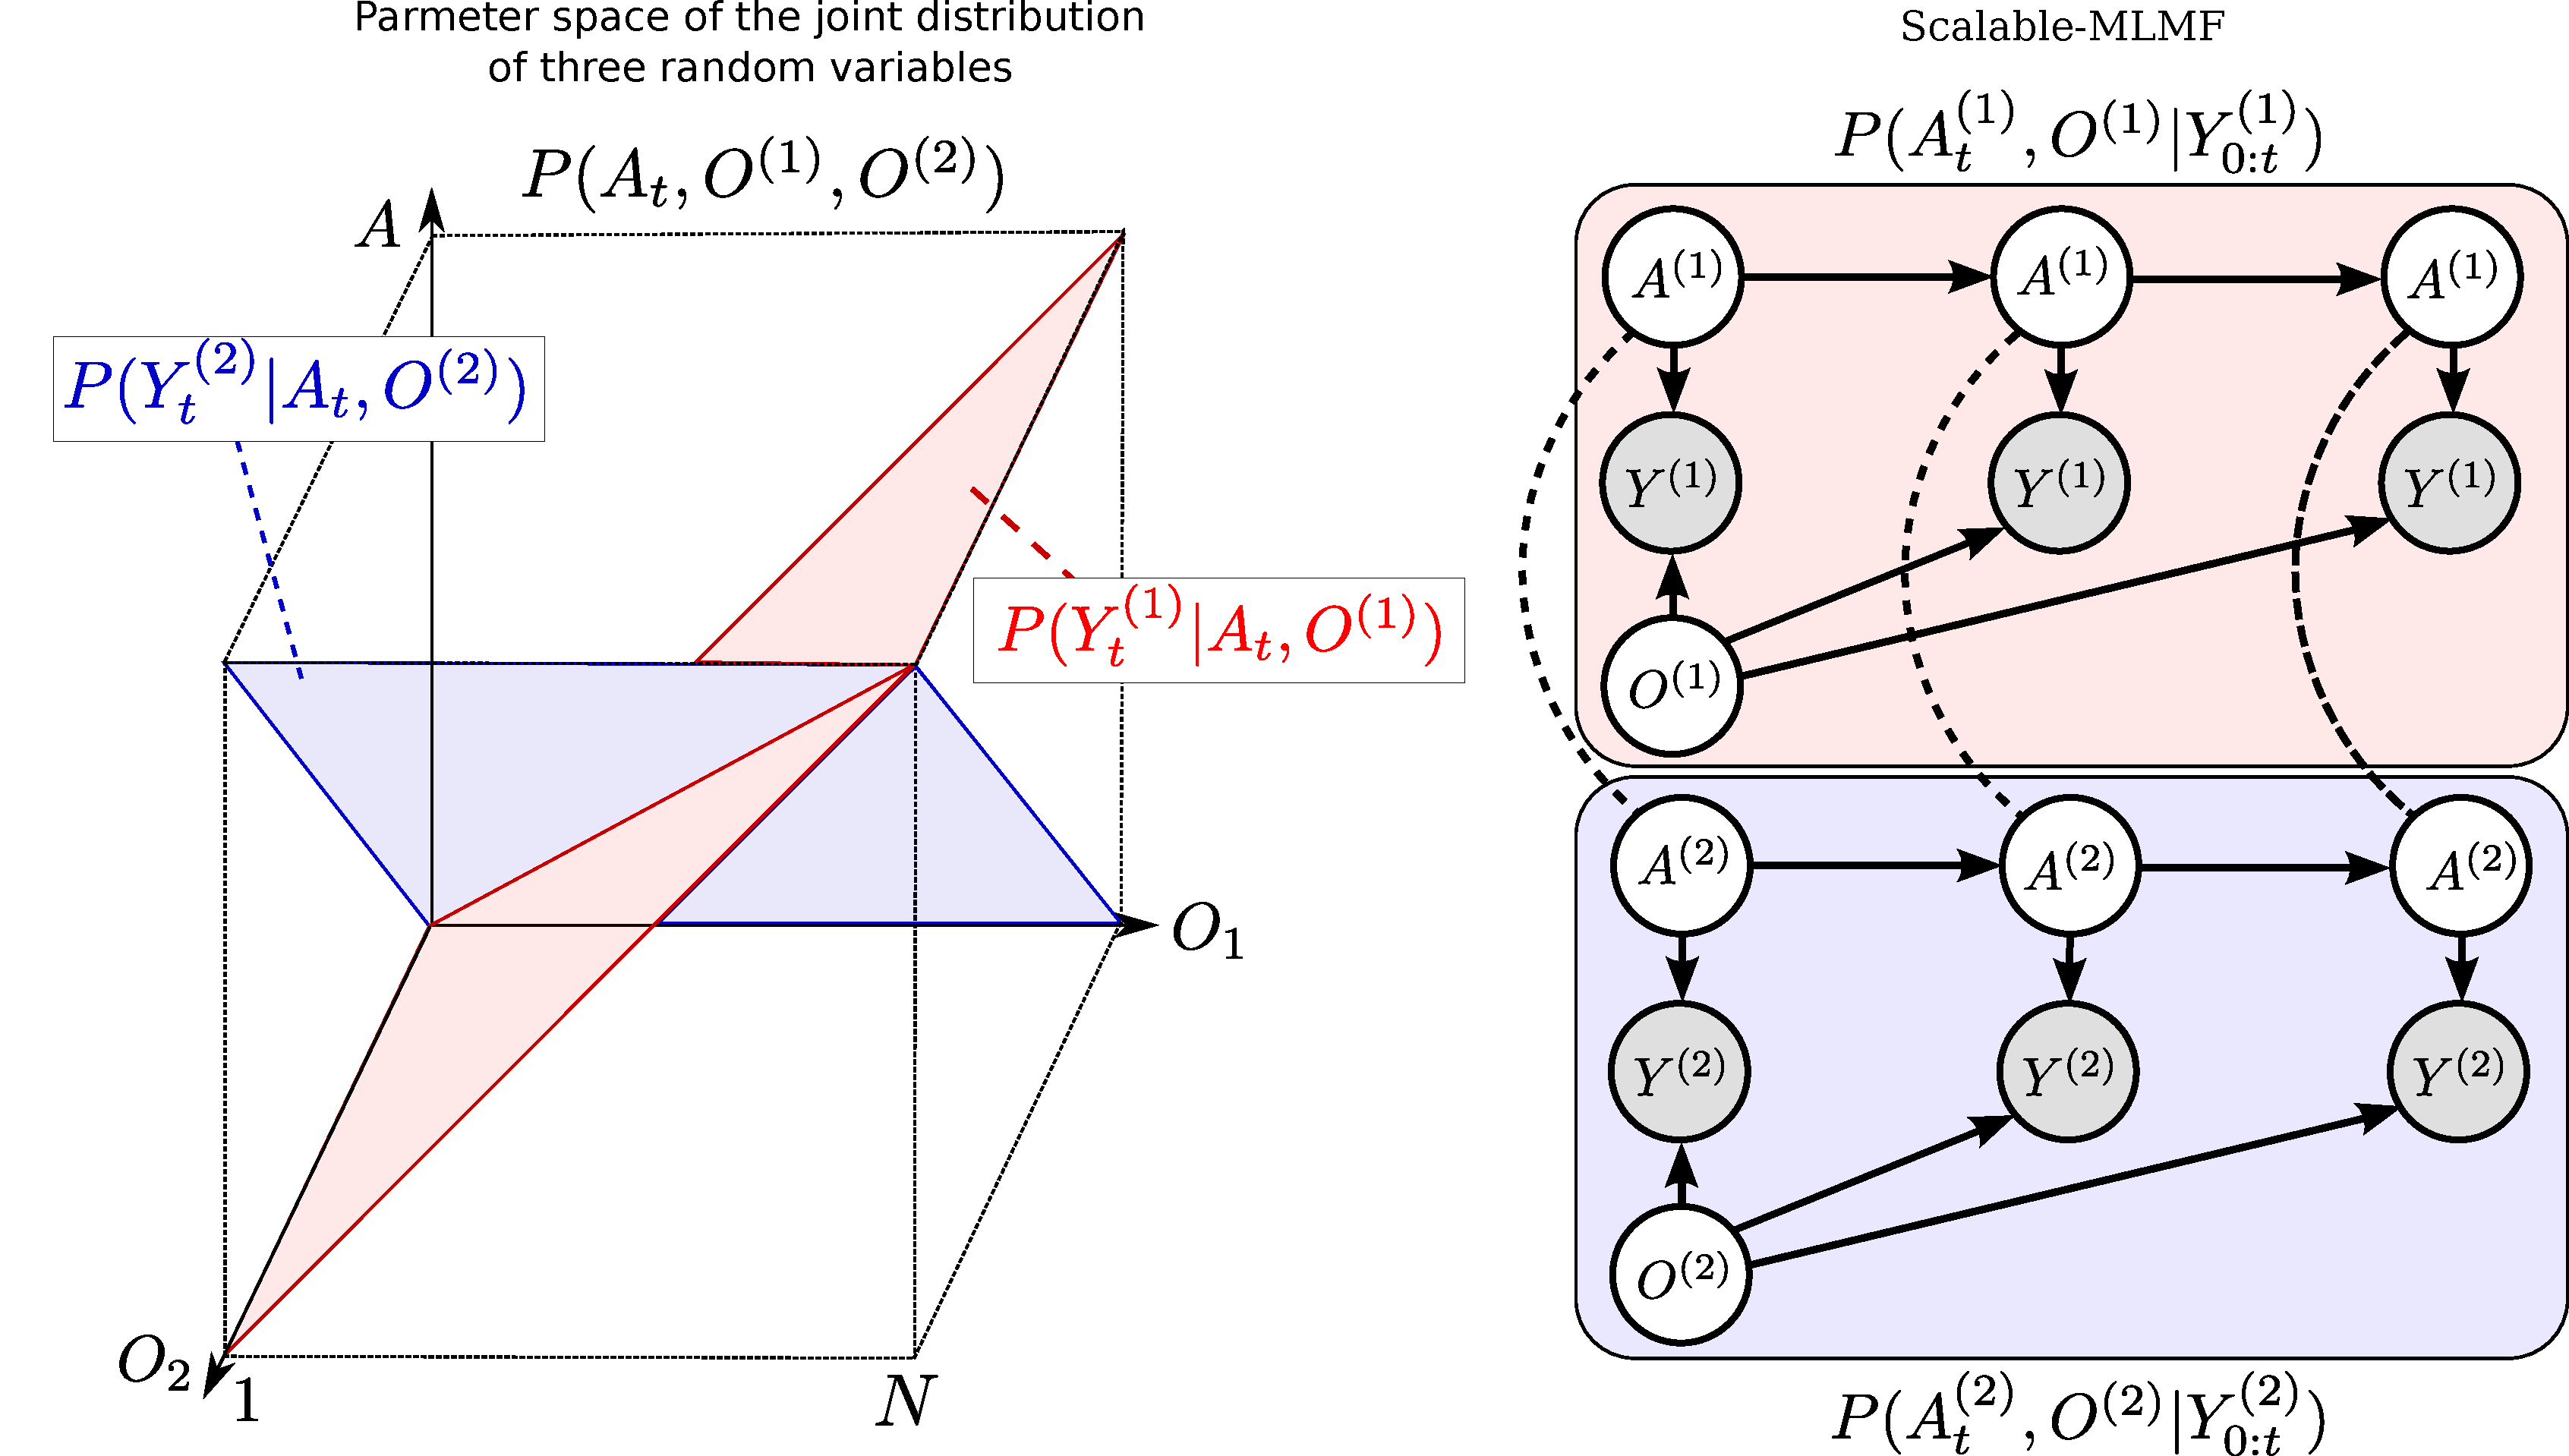
\includegraphics[width=\textwidth]{./ch5-MLMF/Figures/Figure8_v2.pdf}
  \caption{\textit{Left:} Joint distribution $P(A,O^{(1)},O^{(2)})$ of the agent and two objects. Each measurement likelihood function, $P(Y|A,O^{(1)})$, 
  $P(Y|A,O^{(2)})$ corresponds to a hyperplane in the joint distribution
  The state space is discretised to $N$ bins giving the total number of parameters in the joint distribution of $N^3$. 
  \textit{Right:} \textbf{Scalable-MLMF} Each agent-object joint distribution pair is modelled independently. For clarity we have left 
  out the action random variable $u$ which is linked to every agent node.
  Two joint distributions $P(A^{(1)},O^{(1)}|Y^{(1)}_{0:t})$   and $P(A^{(2)},O^{(2)}|Y^{(2)}_{0:t})$ parametrise the graphical model. 
  The dashed undirected lines represent a wanted dependency, if present $O^{(1)}$ and $O^{(2)}$ are to be dependent through $A$. In
  the standard setting there will be no exchange of information between the individual joints. However we demonstrate later on how
  we perform a one time transfer of information when one of the objects is sensed.}
  %\textit{Right:} Joint distribution of the agent and one object $P(A_t,O|Y_{0:t})$.
  %Three measurement 
  %functions have been added to the memory term. At every time step when an action is taken all measurement functions are updated according to 
  %the action applied $u_t$. This means that the first function to be added to the memory will have had all actions applied to it. The number 
  %of the equations and their associated lines in the plot indicate the order in which they have been added to the memory. 
  %The three points are candidates at which we want to evaluate the joint distribution.  The cost of evaluating the 
  %joint distribution at the yellow point is $\BigO(1)$ since we only have to check the first element in the memory. 
  %For the green and cyan points the cost is $\BigO(\log(n))$, where $n$ is the number of likelihood functions in memory.}
  \label{fig:3bel_lik_profile}
\end{figure}

\subsubsection{Time complexity}

For Histogram-SLAM, the computational cost is equivalent to that of the space complexity, $\BigO(N^M)$,
since to obtain all the marginals, every state in the joint distribution has to be summed.

For MLMF-SLAM, every state in the joint distribution's state space which has been changed by the measurement likelihood function 
has to be summed, see Figure \ref{fig:ch5:marginal_update}. As a result the computational complexity is directly related to the number 
of dependent states $|A \cap O|$. In Figure \ref{fig:3bel_lik_profile} \textit{left}, the number of effected states are those in the blue
and red plane (the states in the green plane will only be changed once because the agent's motion is parallel to it).
For $M$ random variables the computational cost is $\BigO(N^{M-1})$ as opposed to $\BigO(N^M)$. 
The computation complexity in this setup is still exponential but to the order $M-1$ as opposed to $M$ which will nevertheless quickly limits 
the scalability as more objects are added. 

%\paragraph{Evaluation of a state in the joint distribution}
%In Figure \ref{fig:3bel_lik_profile} (right) we show three different points in the joint distribution to be evaluated. 
%The memory of applied measurement functions is searched to see if any have effected the values at the three chosen the states. 
%The memory functions are sorted according to their offset from the axis $i=j$. For the yellow point the cost is 
%of $\BigO(1)$ since we only have to check the first (last) element in the list. For the green and blue point the 
%search is $\BigO(\log(n))$, where $n$ is the number of stored memory functions (there can be no more than $N$, the total number of states). 

\subsection{Scalable extension to multiple objects}\label{subsec:scalabe_extension}

To make our filter scalable we introduce an \textbf{independence assumption} between the objects and model 
the joint distribution (Equation \ref{eq:pair_wise_joint}) as the product of agent-object pairs:

\begin{equation}\label{eq:pair_wise_joint}
 P(A_t,O^{(1)},\cdots,O^{(M-1)}|Y_{0:t}) = \prod\limits_{i=1}^{M-1} P(A^{(i)}_t,O^{(i)}|Y^{(i)}_{0:t})
\end{equation}

The measurement variable $Y_t$, is the vector of all agent-object 
measurements, $Y_t = \left[Y^{(1)}_t,\dots,Y^{(M-1)}_t\right]^{\mathrm{T}}$. Each agent-object joint distribution has its own parametrisation of the agent's marginal,
$A^{(1)}_t,\dots,A^{(M-1)}_t$ which combine to give the overall marginal of the agent $A_t$.

%\begin{figure}
%\centering
%  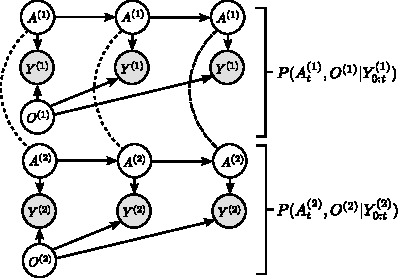
\includegraphics[width=0.5\textwidth]{./ch5-MLMF/Figures/Figure9.pdf}
%  \caption{\textbf{Scalable filter} Each agent-object joint distribution pair is modelled independently. For clarity we have left 
%  out the action random variable $u$ which is linked to every agent node.
%  Two joint distributions $P(A^{(1)},O^{(1)}|Y^{(1)}_{0:t})$   and $P(A^{(2)},O^{(2)}|Y^{(2)}_{0:t})$ parametrise the graphical model. 
%  The dashed undirected lines represent a wanted dependency, if present $O^{(1)}$ and $O^{(2)}$ are to be dependent through $A$. In
%  the standard setting there will be no exchange of information between the individual joints. However we demonstrate later on how
%  we perform a one time transfer of information when one of the objects is sensed.}
%  \label{fig:scalable_mlmf_dae}
%\end{figure}

The computation of each object marginal $P(O^{(i)}|Y^{(i)}_{0:t})$ is independent of the other objects. This is evident from the marginalisation 
see Equation \ref{eq:marg_indep}-\ref{eq:marg_indep_prod}.

\begin{align}
 P(O^{(i)}|Y^{(i)}_{0:t}) &= \sum\limits_{A^{(i)}_t} P(A^{(i)}_t,O^{(i)}|Y^{(i)}_{0:t}) \label{eq:marg_indep} \\
 P(A_t|Y_{0:t})           &= \prod\limits_{i=1}^{M-1} \left(\sum\limits_{O_i} P(A^{(i)}_t,O^{(i)}|Y^{(i)}_{0:t})\right)  \\
	                  &= \prod\limits_{i=1}^{M-1} \ P(A^{(i)}_t|Y^{(i)}_{0:t}) \label{eq:marg_indep_prod}
\end{align}

The independence assumption will create an unwanted effect with respect to agent's marginal $P(A_t|Y_{0:t})$. 
At initialisation the agent marginals should be equal, $P(A_0|Y_0) = P(A^{(i)}_0|Y^{(i)}_0) \forall_i$, however this is not the case because of 
Equation \ref{eq:marg_indep_prod}. To overcome this we define the final marginal, $P(A_t|Y_{0:t})$, of the agent as being the average of all the individual
pairs $P(A^{(i)}|Y^{(i)}_{0:t})$.

\begin{equation}
  P(A_t|Y_t) := \frac{1}{M-1} \sum\limits_{i=1}^{M-1} \ P(A^{(i)}_t|Y^{(i)}_t) \label{eq:marg_indep_sum}
\end{equation}

Figure \ref{fig:3bel_lik_profile} (\textit{Right}), depicts the graphical model of the scalable formulation. 
As each joint distribution pair has its own parametrisation of the agent's marginal and these do not subsequently get updated by one another,
the information gained by one joint distribution pair is \textbf{not transferred}.
A remedy is to transfer information between the marginals $A^{(i)}$ at specific intervals namely when one of the objects is sensed by the agent. 

\begin{center}
\begin{minipage}{\linewidth}

\begin{algorithm}[H]
\label{alg:scalabe-mrf-slam}
\SetKwComment{Comment}{$\triangleright$\ }{}
\SetKwInOut{Input}{input}
\SetKwInOut{Output}{output}
\Input{$P(A^{(i)}_t)$, $P(A^{(i)}_t|Y^{(i)}_{0:t-1})$\\$P(O^{(i)})$, $P(O^{(i)}|Y^{(i)}_{0:t-1})$\\ $Y^{(i)}_t$\\$i=1,\cdots,M$}
\BlankLine

\Comment{If object $i$ has been sensed by the agent}
\eIf{$Y^{(i)}_t > 0$}{
% \Comment*[r]{measurement update Algo. \ref{alg:mrf-slam} }
$P(O^{(i)}|Y^{(i)}_{0:t})   \gets P(O^{(i)}|Y^{(i)}_{0:t-1})$  \Comment*[r]{measurement update Algo. \ref{alg:mrf-slam}} 
$P(A^{(i)}_t|Y^{(i)}_{0:t}) \gets P(A^{(i)}_t|Y^{(i)}_{0:t-1})$\\


\ForAll{$j\in(1,\dots M-1) \setminus i$}
{
$P(A^{(j)}_t|Y_{0:t}) = P(A^{(i)}_t|Y_{0:t})$ \\
$P(A^{(j)}_t) = P(A^{(i)}_t)$\\
$P(O^{(j)}|Y^{(i)}_{0:t}) \leftarrow \sum\limits_{A^{(j)}} P(A^{(j)}_t,O^{(j)}|Y^{(i)}_{0:t})$ \Comment*[r]{object $j$ marginal} 
}

}{

\ForAll{$i\in(1,\dots M)$}{
  measurement update Algo. \ref{alg:mrf-slam}
}
}
\caption{Scalable-MLMF: Measurement Update}
\end{algorithm} 
\end{minipage}
\end{center}


The exchange of information of one joint distribution to another is achieved through the agent's marginals $A^{(i)}$ according to Algorithm \ref{alg:scalabe-mrf-slam}.
The measurement update is the same as previously described in Algorithm \ref{alg:mrf-slam} in the case of no positive measurements of the objects. If the agent
senses an object, all of the agent marginals of the remaining joint distributions are set to the marginal of the joint distribution pair belonging to the positive 
measurement $Y^{(i)}_t$. 

\begin{figure}
  \centering
  \fbox{\includegraphics[width=0.8\textwidth]{./ch5-MLMF/Figures/Figure10.pdf}}
  \caption{\textbf{Transfer of information between joint distributions} \textit{top left and right:} Joint distributions of 
   $P(A^{(1)}_t,O^{(1)}|Y^{(1)})$ and $P(A^{(2)}_t,O^{(2)}|Y^{(2)})$ prior and post sensing. The red and blue lines correspond 
  to the region in which the measurement functions $P(Y^{(1)}_{t}|A^{(1)}_t,O^{(1)})$ and $P(Y^{(2)}_{t}|A^{(2)}_t,O^{(2)})$ will change the joint distributions.
  The dotted black lines are for ease of comparing the joint distributions prior and post sensing.
  \textit{bottom right:}  After the agent has sensed $O^{(2)}$, all the probability mass which was not overlapping the blue line becomes an infeasible
  solution to the agent and object locations. \textit{bottom left:} The constraint imposed by the measurement likelihood function of the second object
  (blue line) is transferred to the joint distribution of the first object according to Algorithm \ref{alg:scalabe-mrf-slam}.
  The result is a change in the joint distribution  $P(A^{(1)}_t,O^{(1)}|Y^{(1)})$, which satisfies the constraints 
  imposed by the agent's marginal from the joint distribution $P(A^{(2)}_t,O^{(2)}|Y^{(2)})$.}
  \label{fig:transfer_information}
\end{figure}

Figure \ref{fig:transfer_information}, depicts the process of information exchange between object $O^{(1)}$ and $O^{(2)}$ in the event that the agent 
gets a positive sensation of $O^{(2)}$. Prior to the positive detection both marginals $P(A^{(1)}_t|Y^{(1)}_{0:t-1})$ and $P(A^{(2)}_t|Y^{(2)}_{0:t-1})$ 
occupy the same region and are identical. When the agent senses $O^{(2)}$ the line defined by the measurement 
likelihood function $P(Y^{(2)}_t|A^{(2)}_t,O^{(2)})$ becomes a hard constraint implying that both the agent and $O^{(2)}$ have to satisfy this constraint.

Figure \ref{fig:independence_object} shows marginals resulting from the joint distributions in Figure \ref{fig:transfer_information}. The marginals in
the \textit{left} plot are the result after updating the marginals $A^{(i)}$. The \textit{right} plot shows the result for the case where the objects
remain independent. 

The result of introducing a dependency between the objects through the agent's marginals in the event of a sensing and treating them
independently gives the same solution as the histogram filter in this particular case. However as each individual marginal $A^{(i)}_t$ diverges 
from the other marginals the filtered solution will diverge from the histogram's solution. We assume however that the objects are weakly dependent 
and sharing information during positive sensing events would be sufficient. In section \ref{subsec:eval_indep_assumptiom} we will 
evaluate the independence assumption with respect to the histogram filter.

Table \ref{tab:time_space_summary} summarises the time and space complexity for the three filters.% In the case of transfer of
%information between marginals the computational complexity is higher, however this is a one time occurrence. 

\begin{figure}
  \centering
  \fbox{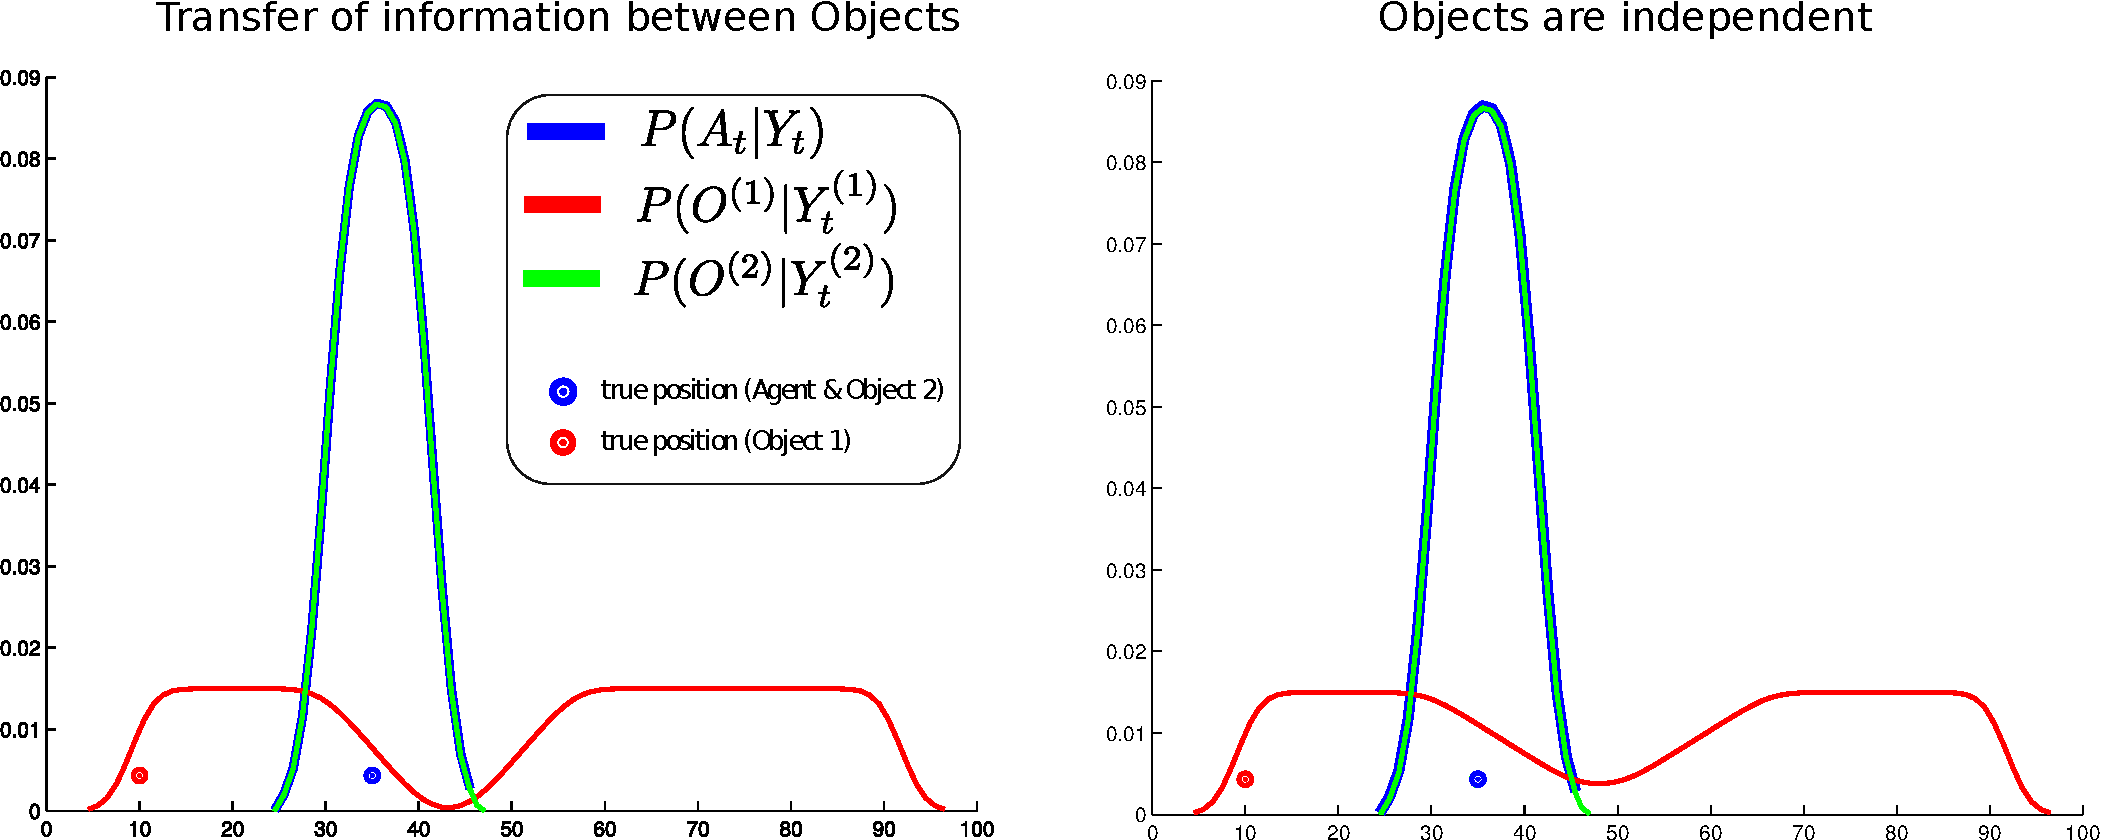
\includegraphics[width=0.8\textwidth]{./ch5-MLMF/Figures/Figure11.pdf}}
  \caption{\textbf{Independence \& Objects} \textit{left:} resulting marginals after setting the agent marginals of each pair wise joint distribution
  equal $A^{(1)}_t = A^{(2)}_t$ according to Algorithm \ref{alg:scalabe-mrf-slam}. The object marginal $P(O^{(2)}|Y_{0:t})$ is recomputed. 
  \textit{right:} resulting marginals in which the objects have no influence on one another. The difference
   between the two figures is that the object $O^{(1)}$ marginal changed in the case where we introduced the dependence \textit{left plot}, and remained 
  unchanged in the case where the objects are treated as being independent \textit{right plot}.}
  \label{fig:independence_object}
\end{figure}


%For the full derivation of time and space complexity of the scalable-MLMF filter see Appendix \ref{appendix:space_time_scalable_mlmf}.

\begin{table}
 \centering
 \begin{tabular}{c|c|c|}
\cline{2-3}
				        &    \textbf{space}   &     \textbf{time} \\ \hline
    \multicolumn{1}{|l}{Histogram}      & \multicolumn{1}{|l}{$\BigO(N^M)$}   &  \multicolumn{1}{|l|}{$\BigO(N^M)$}      \\ \hline
    \multicolumn{1}{|l}{MLMF}           & \multicolumn{1}{|l}{$\BigO(M\,N)$}  &  \multicolumn{1}{|l|}{$\BigO(N^{(M-1)})$} \\ \hline
    \multicolumn{1}{|l}{scalable-MLMF}  & \multicolumn{1}{|l}{$\BigO(M\,N)$}  &  \multicolumn{1}{|l|}{$\BigO(M\,N)$}     \\ \hline
   \end{tabular}
   \caption{\textbf{Time and space complexity summary} For both MLMF and scalabe-MLMF the worst case scenario is reported for the space complexity.}
   \label{tab:time_space_summary}
\end{table}



\section{Evaluation}\label{ch5:evaluation}

We conduct three different types of evaluation to quantify the scalability and correctness of the scalable-MLMF filter. The first experiment
tests the scalability of our filter in terms of processing time taken per motion-measurement update cycle. The second experiment evaluates the independence 
assumption between the objects which was made in the scalable-MLMF filter. The third and final experiment determines the effect the memory size has 
on a search policy whose goal is to locate all the objects in the \textit{Table} world.

\subsection{Evaluation of time complexity}

We measured the time taken by the motion-measurement update loop, as a function of the number beliefs and number of states per belief. 
We started with a 100 states per belief and gradually increase it to 10'000'000 over 50 steps. For each of the 50 steps we went from 2 objects to 25. Figure \ref{fig:time_complexity} \textit{left} illustrates the computational
cost as a function of number of states and objects. For each state-object pair 100 motion-measurement updates were performed. Most of the trials returned time updates 
below 1 Hz. Figure \ref{fig:time_complexity} \textit{right} shows the computational cost as a function of the number of states plotted for 6 different filter runs with
a different number of objects. As the number of states increases exponentially so does the computational cost. Note the cost increases at the same
rate as the number of states meaning that the computational complexity is linear with respect to the number of states. This result is in agreement with 
the asymptotic time complexity.

\begin{figure}
 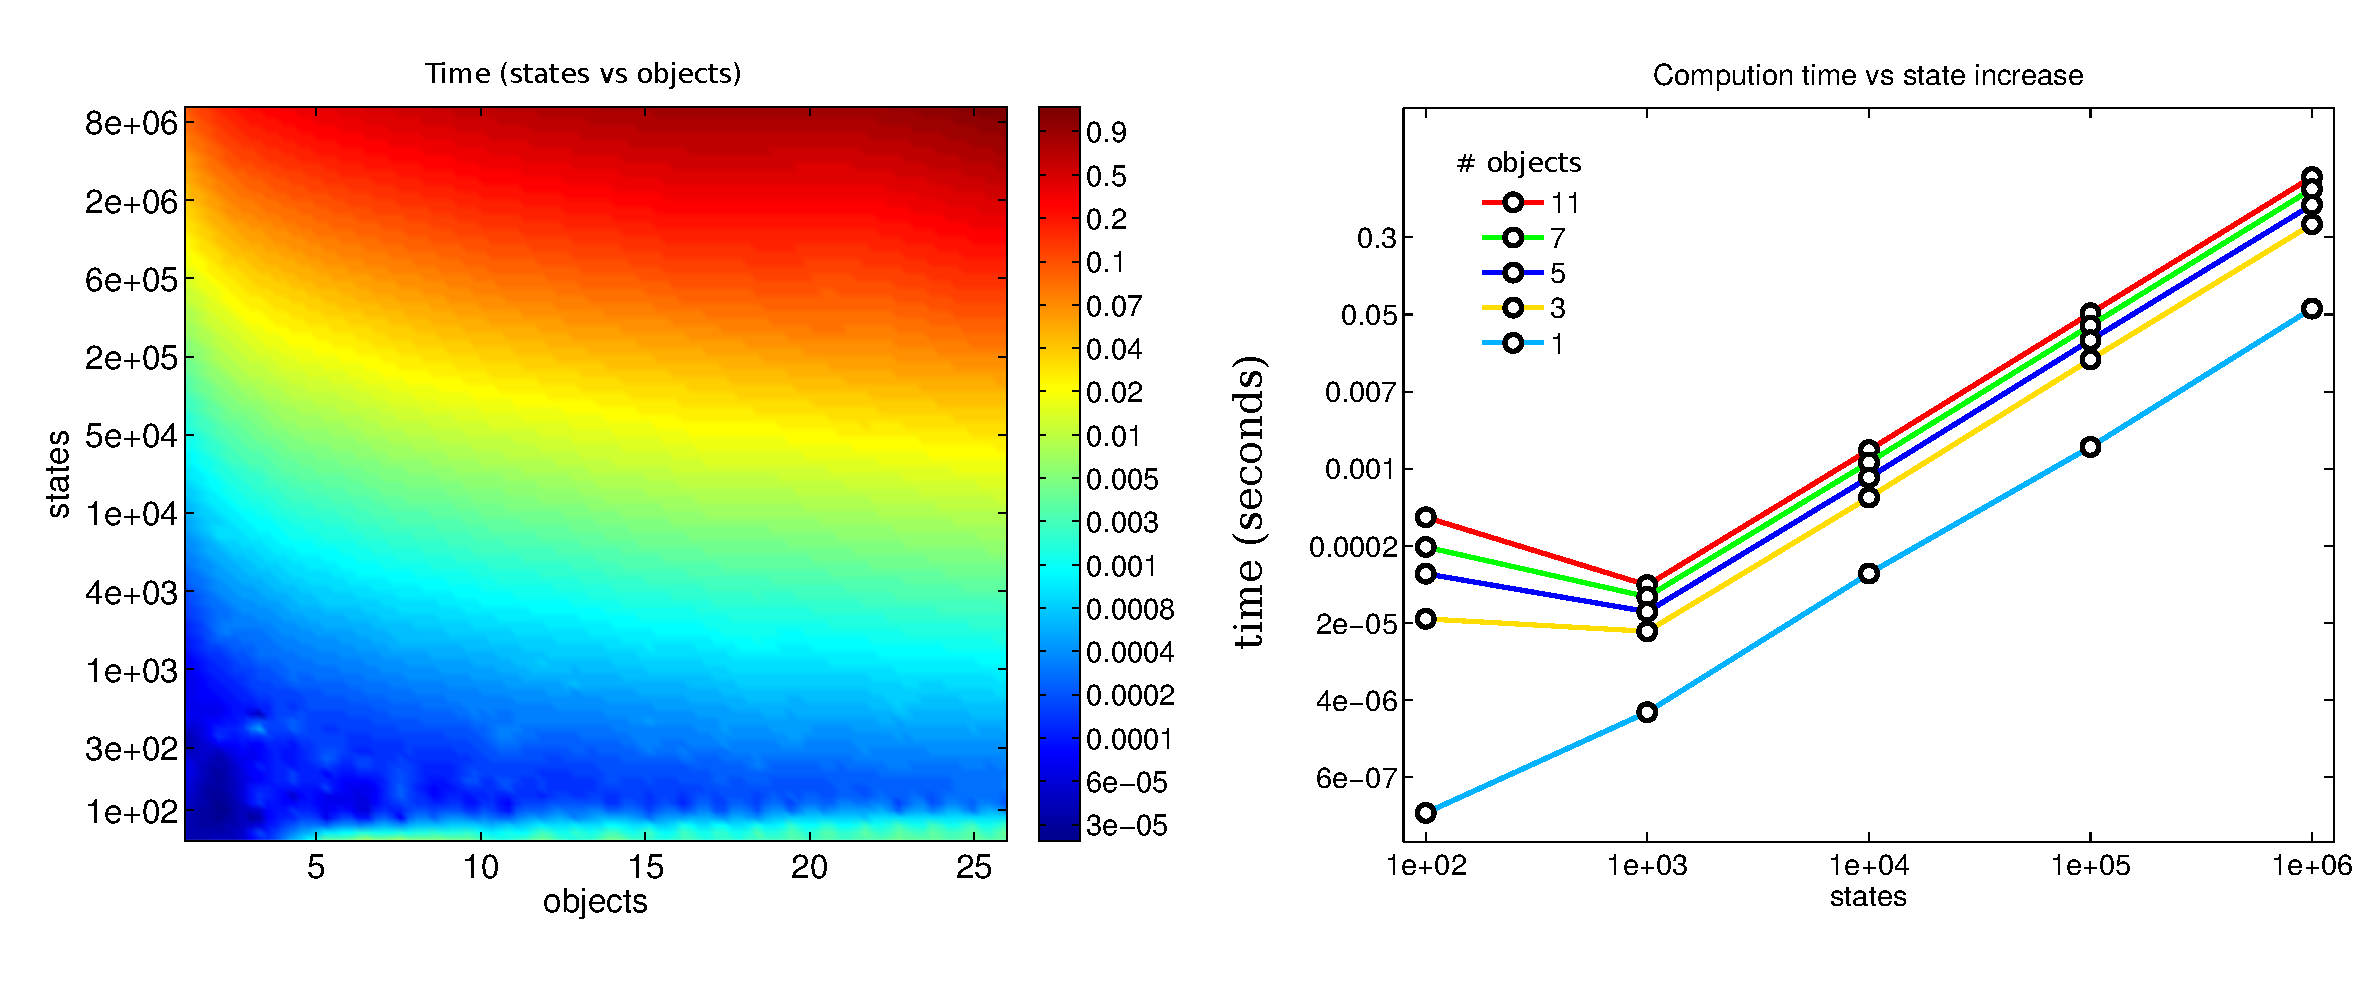
\includegraphics[width=\textwidth]{./ch5-MLMF/Figures/Figure12_v2.pdf}
 \caption{\textbf{Time complexity:} \textit{left:} mean time taken for a loop update (motion and measurement) as a function of the number of states in a marginal and the 
 number of objects present. \textit{right:} time taken for a loop update with respect to the number of states in the marginal. The colour coded lines are 
 associated with the number of objects present. The computational cost is plotted on a log scale. As the number of states increases exponentially the
 computational cost matches it.}
 \label{fig:time_complexity}
\end{figure}


\subsection{Evaluation of independence assumption}\label{subsec:eval_indep_assumptiom}

In section \ref{subsec:scalabe_extension} we made the assumption (for scalability reasons) that the objects' beliefs are independent
of one another. This assumption is validated by comparing the MLMF filter on three random variables, an agent and two objects, with the ground truth
which we obtain from the standard histogram filter. For each of the three beliefs (the agent and two objects), 100 different marginals 
were generated and the true locations (actual position of the agent and objects) were sampled. 
The agent carries out  a sweep of the state space for each of the 100 initialisations and the actual policy is saved 
and run with the scaled-MLMF filter. In the first experiment we assume that the objects are completely independent 
and that there is no transfer of information between the pair-wise joint distributions. In the second and third experiments there 
is an exchange of information as described in Algorithm \ref{alg:scalabe-mrf-slam}. Here we compare the effect of using the product of the agent's marginals $P(A_t|Y_{0:t}) = P(A^{(1)}_t|Y^{(1)}_{0:t}) \cdot P(A^{(2)}_t|Y^{(2)}_{0:t})$ 
against their average $P(A_t|Y_{0:t}) = \frac{1}{2}P(A^{(1)}_t|Y^{(1)}_{0:t}) + \frac{1}{2}P(A^{(2)}_t|Y^{(2)}_{0:t})$. 

For each of the 100 sweeps the ground is compared with the histogram filter and scalabe-MLMF using the Hellinger distance (Equation \ref{eq:hellinger}).
\begin{equation} \label{eq:hellinger}
 H(P,Q) = \frac{1}{\sqrt{2}}\, \|\sqrt{P} - \sqrt{Q}\|_2  
\end{equation}
The Hellinger distance is a metric which measures the distance between two probability distributions. Its value lies strictly between 0 (the two 
distributions are identical) and 1 (no overlap between them). Figure \ref{fig:independence_assumption_test} shows the kernel density 
distribution of the Hellinger distances taken at each time step for all 100 sweeps.

The best results were for case 3). The \textit{bottom plots} show that the Hellinger distance distribution between the
object marginals for both case 2) and 3) are the same. However there is a significant improvement when using the average of the agent's marginals as oppose to 
their product. 

\begin{figure}
 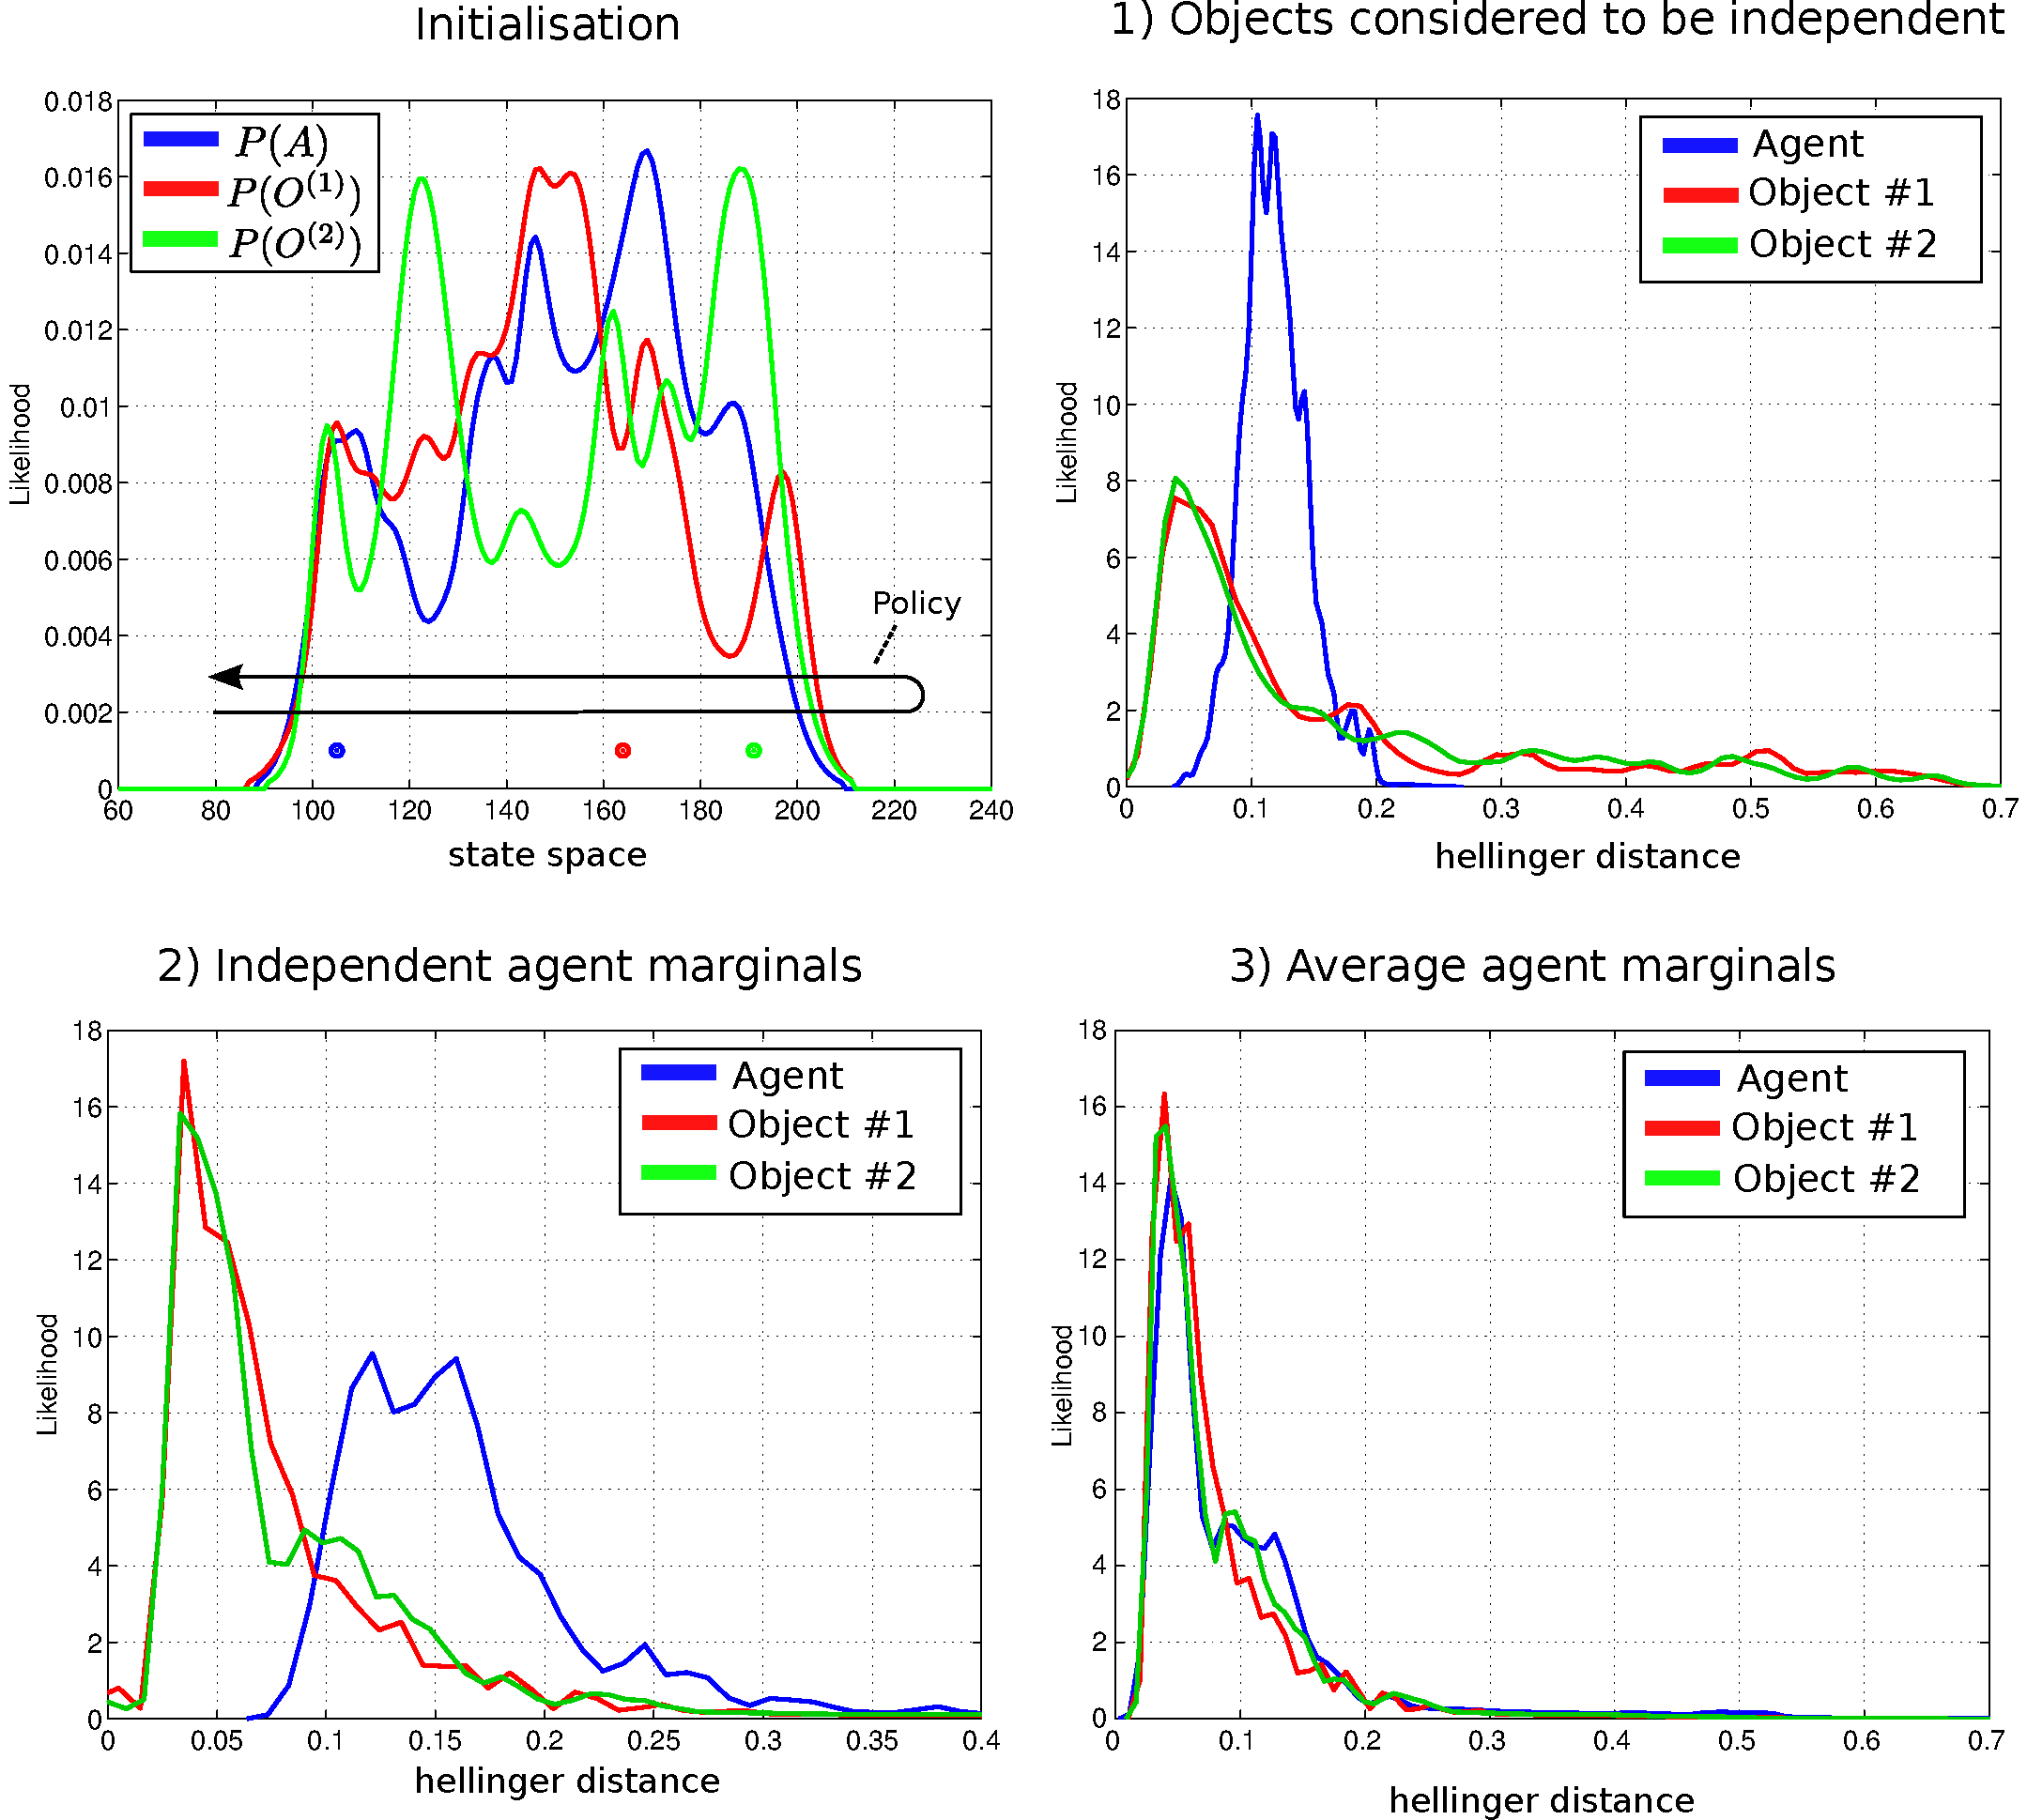
\includegraphics[width=\textwidth]{./ch5-MLMF/Figures/Figure13.pdf}
 \caption{\textbf{Comparison of scalable-MLMF and the histogram filter} A deterministic sweep policy was carried out for 100 different initialisations of 
 the agent and object beliefs. \textit{top left:} One particular Initialisation of the agent and object
 random variables. The true position of the agent and objects were sampled at random. The black arrow indicates the general policy which was 
 followed for each of the 100 sweeps. 
 These were performed for 1) scalable-MLMF  with objects considered to be independent at all times (no Algorithm \ref{alg:scalabe-mrf-slam}). 2) 
 Agent marginal $P(A_t|Y_{0:t})$ is the product of marginals $P(A^{(i)}_t|Y^{(i)}_{0:t})$ (Equation \ref{eq:marg_indep_prod}). 
 3) marginal $P(A_t|Y_t)$ is taken to be the average 
 of all marginals $P(A^{(i)}_t|Y^{(i)}_{0:t})$ (Equation \ref{eq:marg_indep_sum}).  For each of these three experiment we report the 
 kernel density estimation over the Hellinger distances taken at every time step between ground truth (from histogram filter) and scalable-MLMF.}
 \label{fig:independence_assumption_test}
\end{figure}

\subsection{Evaluation of memory}

The memory is the list of all measurement likelihood functions which have been applied on the joint 
distribution since initialisation. As detailed previously there can be no more than $N$ different measurement likelihood functions added to 
memory. In the case of a very large state space this might be cumbersome. We investigate how restricting the memory size 
can impact on the decision process in an Active-SLAM setting. Given our set up we choose a breadth-first search in the action 
space with a one time step horizon, making it a greedy algorithm. The objective function we utilise is the information
gain of the beliefs after applying an action (Equation \ref{eq:greedy_algorithm}).

\begin{equation}\label{eq:greedy_algorithm}
 u_{t} = \operatorname*{arg\,max}_{u_t} H\{P(A_{t-1},O|Y_{0:t-1},u_{1:t-1})\} - \mathbb{E}_{Y_t}\left[H\{P(A_{t},O|Y_{0:t},u_{1:t})\}\right]
\end{equation}

For each action we run the filter forward in time and considered all future measurements since we cannot know ahead of time the actual 
measurement. The information gain is the difference between the current entropy (defined 
by $H\{\cdot\}$) and the future entropy after the simulated motion and measurement update. The action with the highest information gain 
is subsequently selected. This is repeated at each time step. In Figure \ref{fig:exploration_init} we illustrate the environment setup for 
a 1D and 2D case. The agent's task is to find the objects in the environment.


\begin{figure}
  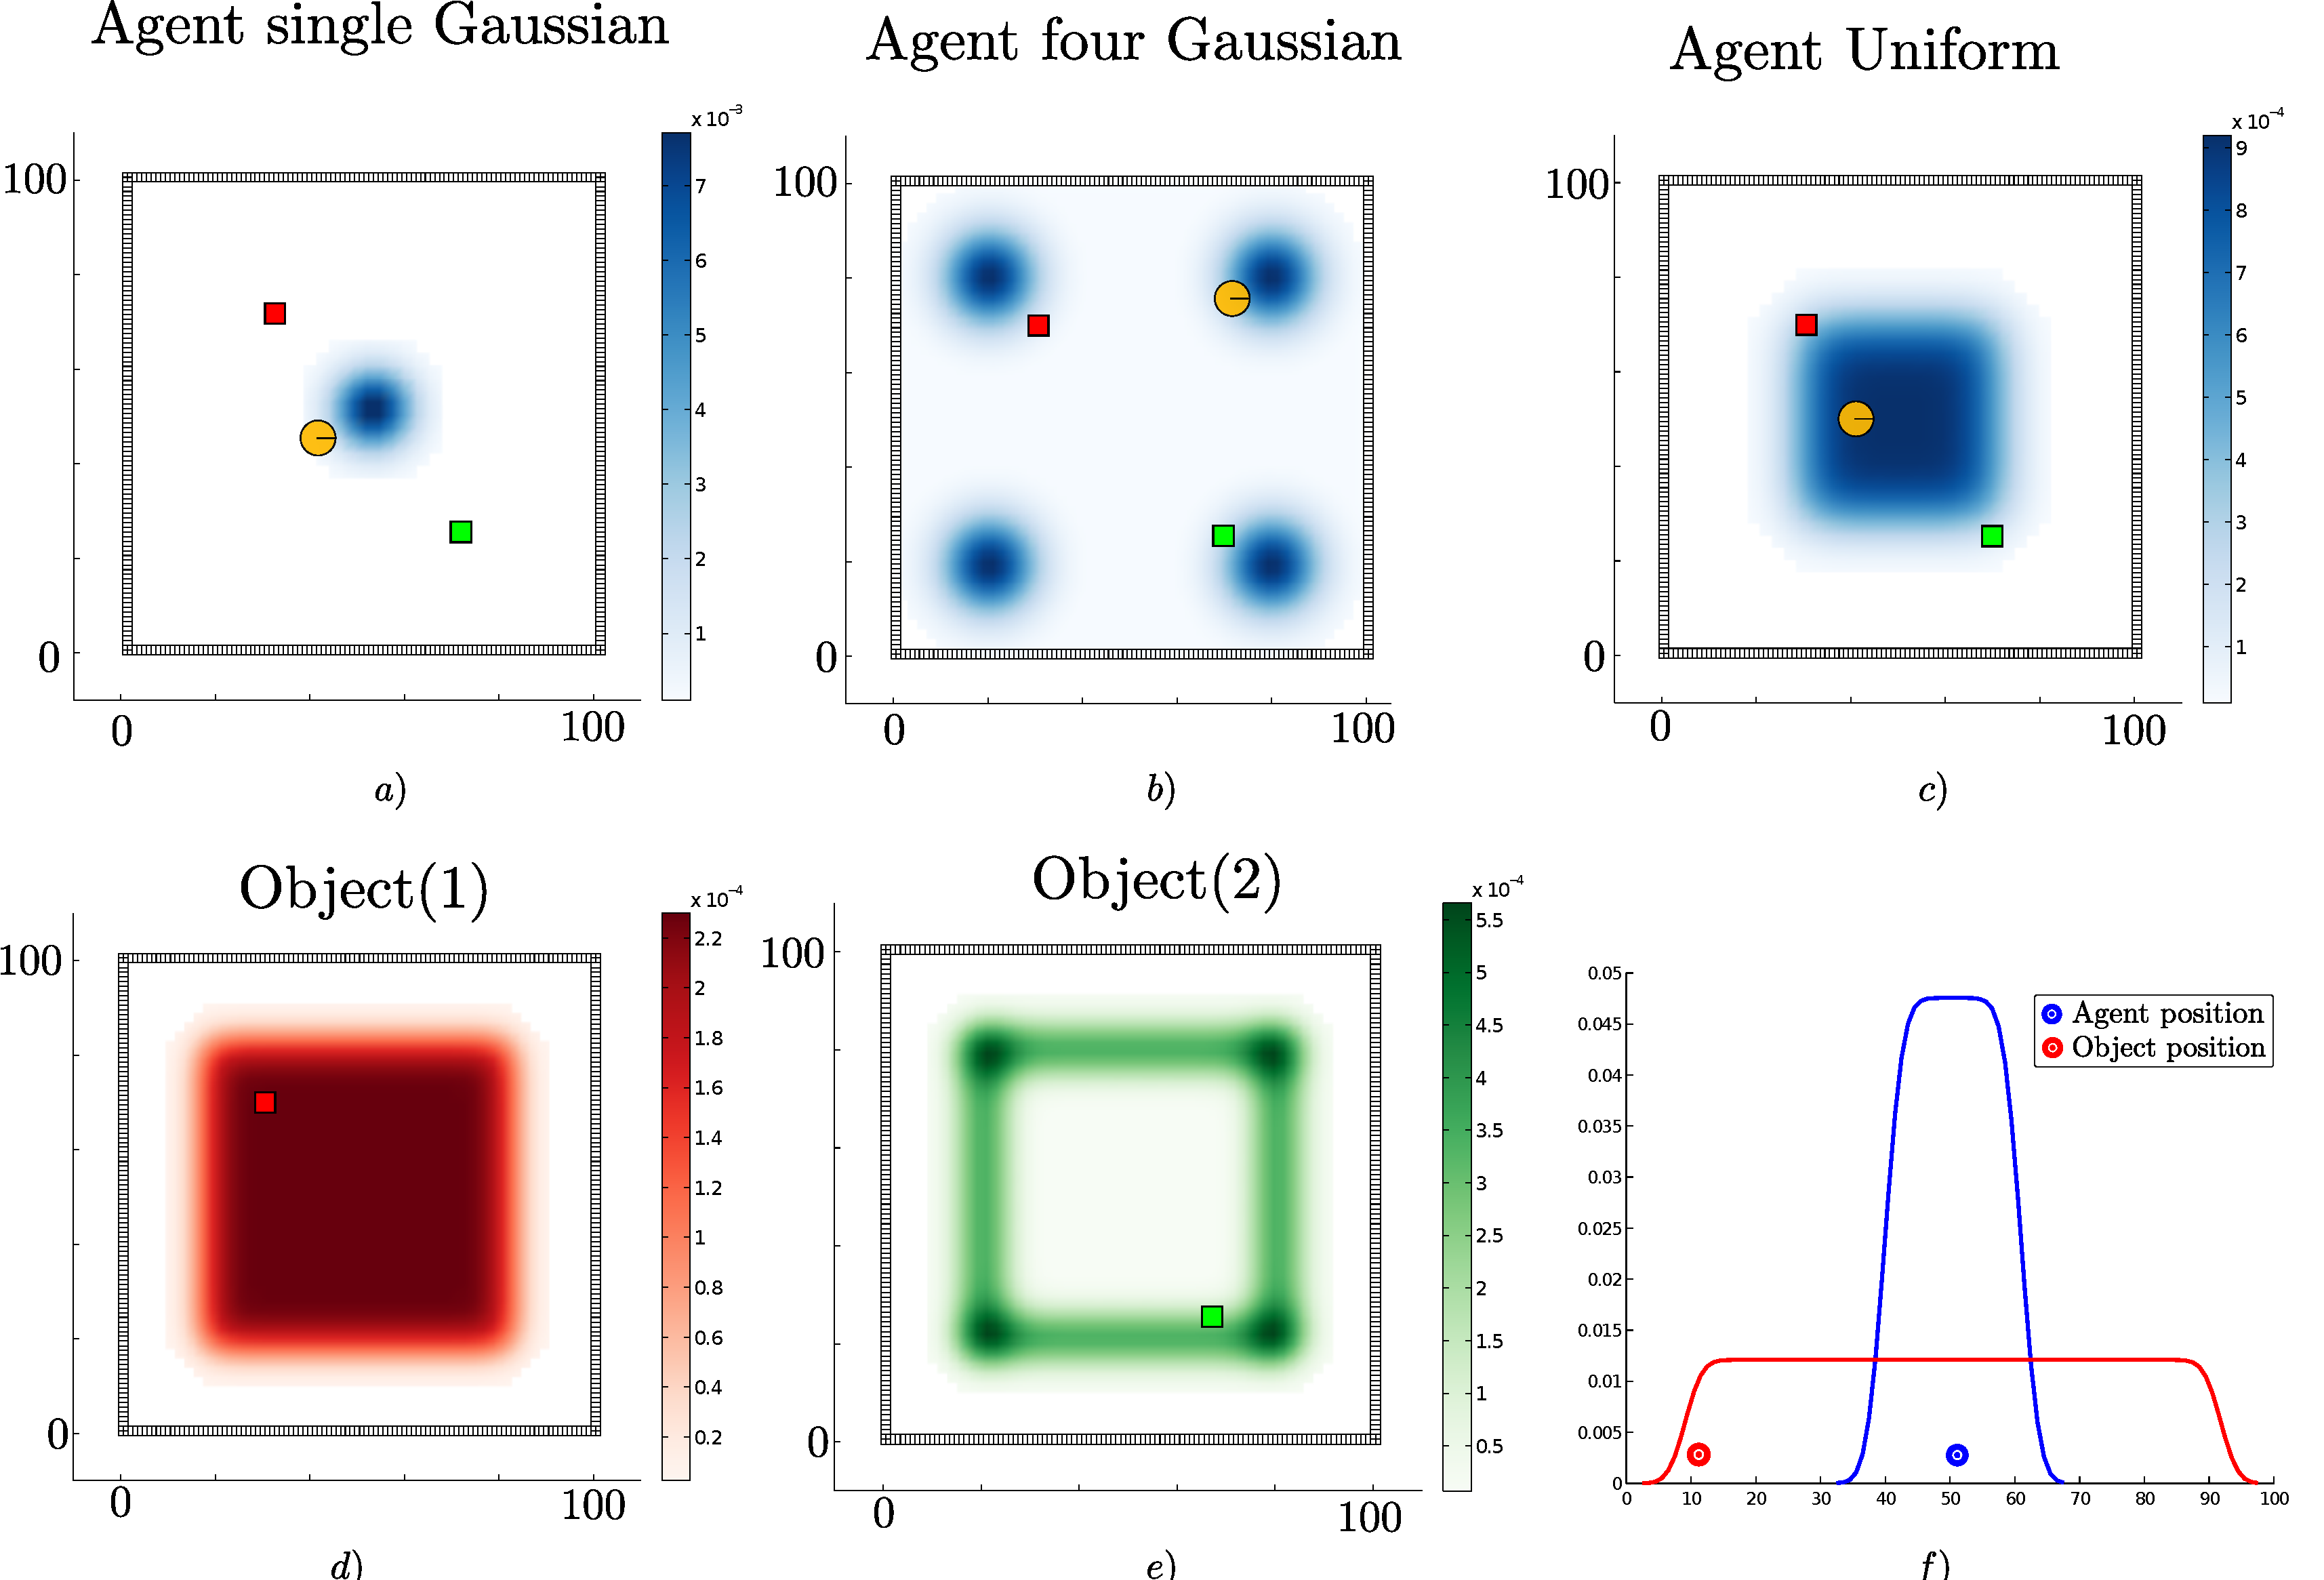
\includegraphics[width=\textwidth]{./ch5-MLMF/Figures/Figure14.pdf}
  \caption{\textbf{Agent's prior beliefs.} Two types of environment, the first is 
  a 2D world in which the agent lives in a square surrounded by a wall whilst the second is a 1D
  world. In the 2D figures the agent is illustrated by a circle with a bar to indicate its heading. The true location 
  of the objects are represented by colour coded squares. \textit{Top row} three different initialisations of the agent's location. 
  \textit{Bottom row} d) the agent's prior beliefs with respect to the location of the first object and e) belief of the second object's location.
  \textit{bottom row} f) 1D world with one object.}
  \label{fig:exploration_init}
\end{figure}

For the 2D search we consider three different initialisations (single-Gaussian, four-Gaussian, Uniform) for the agent's belief where there are 
two objects to be found. Ten searches were carried out for each of the three initialisations of the agent's beliefs. 
The true location of the agent, for each search, is sampled from its initial belief and the objects' locations 
(red and green squares in Figure \ref{fig:exploration_init}) are kept fixed throughout all searches. We repeat each search for 18 different memory 
sizes going from 1 to $N$ (the number of states). For the 1D search case we consider 1 object since adding more objects will make the search easier. 
We are interested in how the memory effects the search and not the search itself. In Figure \ref{fig:time_to_reach_goal} we report on the time taken to 
find all objects with respect to a given memory size which is shown as the percentage of the total number of states. 
In the 1D search case the variability of time taken to find the object converges when the memory size is at 60\% of the original state space. 
As for the 2D search with 2 beliefs (agent \& 1 object) the convergence depends on the agent's initial belief. For the 1-Gaussian (green line) 
all searches take approximately the same amount of time after a memory size of 9\%. As for the remaining two initialisations convergence is achieved at  48\%. 
The same holds true for the case of 3 beliefs (agent \& 2 objects).

In the 2D searches, the size of the memory has a less drastic impact than in the 1D (which is a special search case). 
In the 2D case only when the memory size is less than 6\% is there a significant impact in terms of the time taken to find 
the objects. We conclude that at least in the case of the greedy one step-look ahead planner which is frequently used in the literature, the 
size of the memory seems not to be a limiting factor in terms of the time taken to accomplish the search.


\begin{figure}
  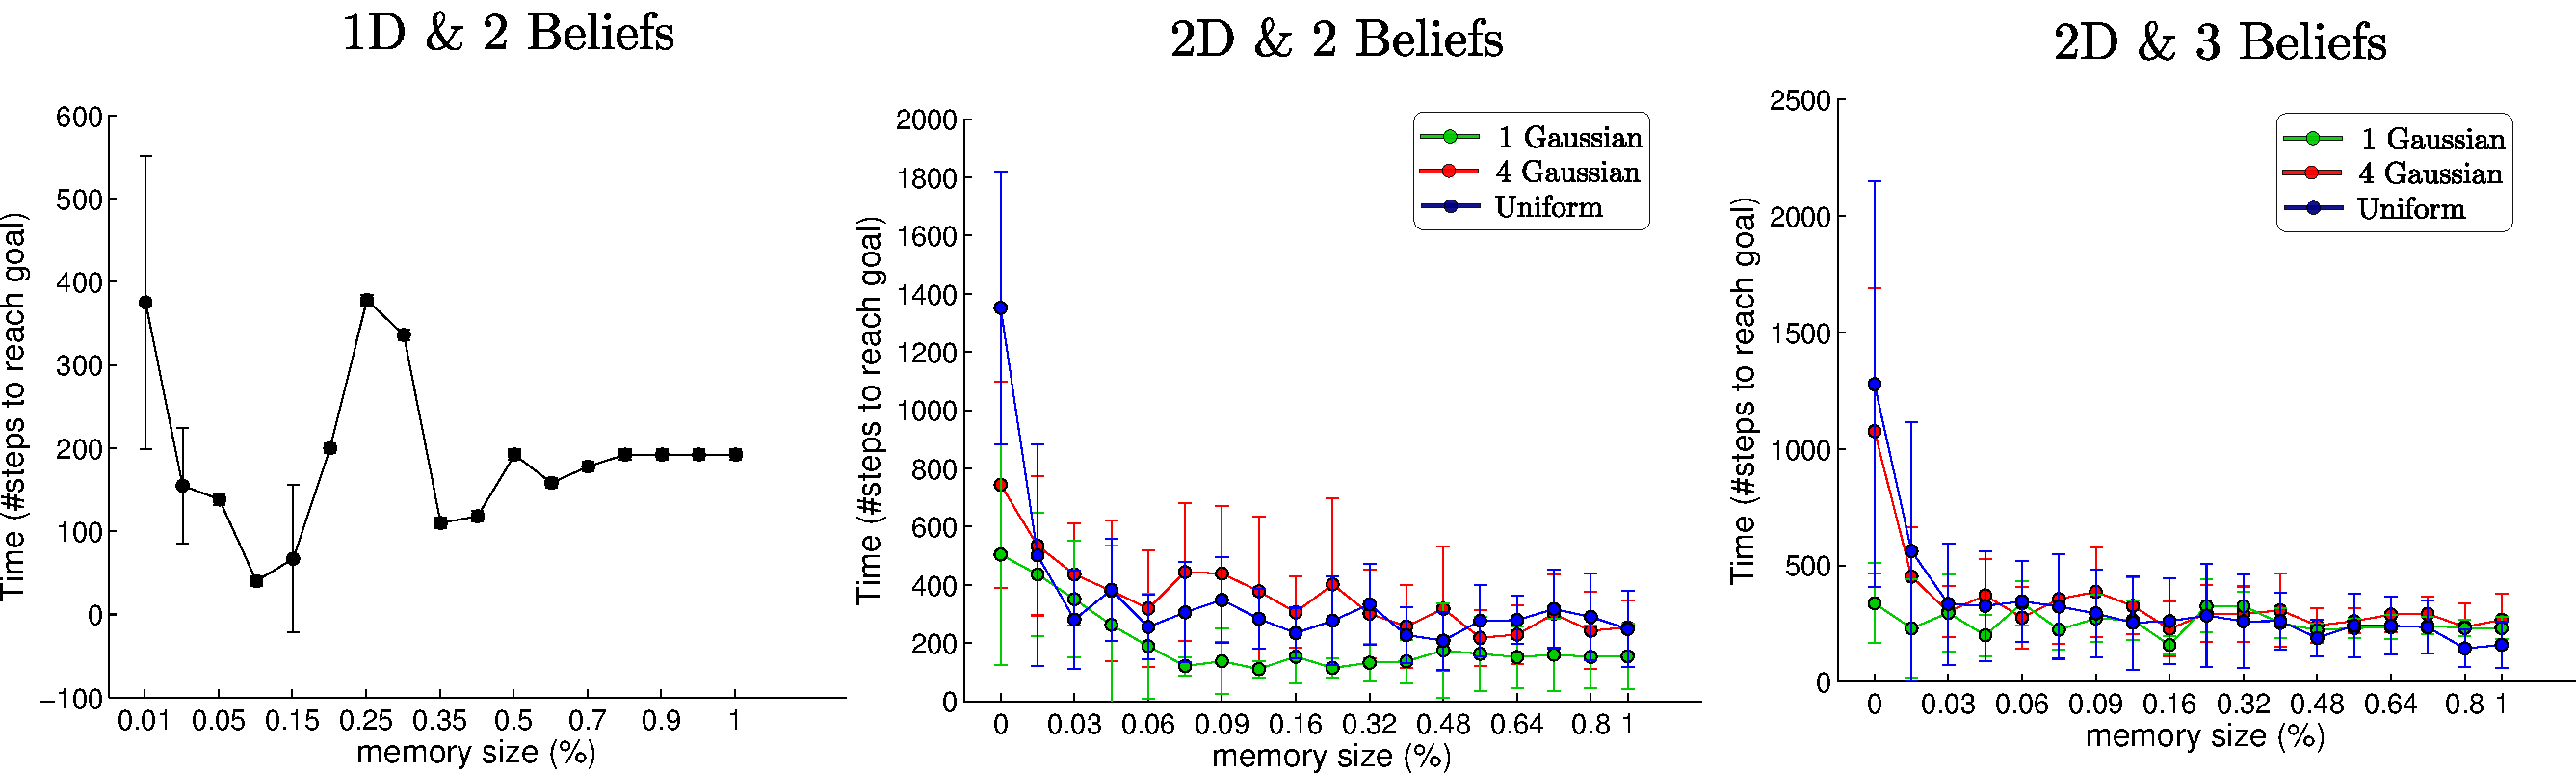
\includegraphics[width=\textwidth]{./ch5-MLMF/Figures/Figure15.pdf}
  \caption{\textbf{Memory size vs time to find objects} Results of the effect of the memory size on the decision process.
  The memory size is reported as the percentage of total number of states present in the marginal space. At 100\% the size
  of the memory is equal to that of the state space. \textit{left:} results of the 1D search illustrated in Figure \ref{fig:exploration_init} \textit{f)}.
  \textit{Middle \& right:} 2D search with initialisations accordingly depicted in Figure \ref{fig:exploration_init}.
  }
  \label{fig:time_to_reach_goal}
\end{figure}

\FloatBarrier
\section{Conclusion}\label{ch5:conclusion}

This work addresses the Active-SLAM filtering problem for scenarios in which sensory information relating to the map is very limited. Current
SLAM algorithms filter the errors originating from sensory measurements and not prior uncertainty. By making the assumption
that the joint distribution of all the random variables is a multivariate Gaussian, inference is tractable. Since the origin of 
our uncertainty is not originating from the measurement noise we cannot assume the joint distribution to have any special structure. 
A suitable filter for such purposes is the histogram which makes no assumption about the shape or form taken by the joint distribution. 
The drawback of this form of parametrisation is that the space and time complexity are exponential with respect to the number random variables 
and this is a major limiting factor for scalability. 

The main contribution of this work is a formulation of a histogram Bayesian state space estimator in which the computational complexity is 
both linear in time and space. We took a different approach to other SLAM formulations in the sense that we did not
explicitly parametrise the joint distribution but kept all parametrisation in the space of the marginals (beliefs),
avoiding the exponential increase in parameter space which would otherwise have been the case. Our filter's parameters 
consist of the marginals and the history of measurement functions which have been applied. By evaluating the joint 
distribution solely at the states which are affected by the current measurement function whilst taking into account the 
memory, the MLMF filter can recover exactly the same filtered marginals as the histogram filter. The worst case space complexity is 
linear rather than exponential and the time complexity remains exponential but grows at a slower rate than in the histogram filter.
In striving to make the filter scalable we assume an independence assumption between the objects. An individual MLMF filter
was used for each agent-object pair. We evaluated the difference between the scalable-MLMF filter with a ground truth provided 
by the histogram filter for 100 different searches with respect to the Hellinger distance. We concluded that 
the divergence was relatively small and thus the scalable-MLMF filter provides a good approximation to the true filtered
marginals. We evaluated the time taken to perform a motion-update loop for different discretisation of the state space (100 to 10'000'000 states) and 
number of objects (2 to 25) present. In most of the cases we achieved an update cycle rate below 1Hz. We evaluated how the increase of the number of states 
effected the computational cost. The relationship was found to be linear and thus is in agreement with our analysis of the asymptotic growth rate. 
We analysed of the effect the memory size (the remembered number of measurement likelihood functions) on the decision theoretic process of reducing
the uncertainty of the map and agent during a search task. We found that in the 2D case the memory size has much less effect than in the 1D case
and we conclude that it is unnecessary to remember every single measurement function.

The implications of the MLMF and scalable-MLMF filter are that we have a computationally tractable means of 
performing SLAM in a case scenario in which mostly negative information is present and the 
joint distribution cannot be assumed to have any specific structure. The filter can be used at a higher cognitive level than 
processing raw sensory information as it is often in Active-SLAM. It would be well suited for reasoning tasks 
where the robot's field of view is limited.

An interesting future extension would be to make the original MLMF filter scalable without introducing assumptions.
One possibility could to be to consider Monte Carlo integration methods for inference. These can scale well to high dimensional 
spaces whilst still providing reliable estimates. A second possibility could be to investigate the use of Gaussian Mixtures as a 
form of parameterisation of the marginals so that it might be possible to blend our filter with  
EKF-SLAM. This would allow the parameters to grow quadratically with respect to the dimension of the marginal space as opposed to
exponentially as it is in the case with the histogram and MLMF filters.



\section{Appendix}\label{ch5:appendix}

%\subsection{EKF-SLAM models}
%\paragraph{Motion update}
%\begin{align}
%  \bar{\mu}_t      &= f(\mu_{t-1},u_t)\\
%  \bar{\Sigma}_{t} &= F \Sigma_{t-1} F^{\mathrm{T}} + Q
%\end{align}
%Where $F = \left[\frac{\partial f(\mu_{t-1},u_t)}{\partial \mu_{t-1} } \right]$ is the Jacobian of the dynamic model with respect to the Gaussian mean. The 
%bar notation on the mean and covariance is to indicate that no sensing information has been used to update their estimates.
%\paragraph{Measurement update}
%\begin{align}
%   K    &= \bar{\Sigma}_{t} H (H \bar{\Sigma}_{t} H + R)^{-1} \\
%  \mu_t &= \bar{\mu}_t + K \cdot (Y_t - \hat{Y}_t)\\
%  \Sigma_t &= (I - KH) \bar{\Sigma}_{t}
%\end{align}
%Where $H = \left[\frac{\partial h(\mu_A,\mu_O;\beta)}{\partial \mu_A\mu_O}\right]$ is the Jacobian of the measurement function (Equation \ref{eq:ekf-measurement_function})  
%with respect to the mean of the joint distribution. 

%\subsection{Bayesian joint to filter}\label{appendix:bayes_joint}
%\begin{align}
%&P(A_t,O,Y_{0:t},u_{1:t})\\
%&= P(O) \left( \sum_{A_{0:t-1}}  P(A_0) \prod_{t=0}^{t} P(A_t|A_{t-1},u_{t}) P(Y_t|A_t,O) \right)  P(Y_t|A_t,O) \\
%&= P(O) \left( \sum_{A_{0:t-1}} P(A_{0:t},Y_{0:t-1},u_{1:t}) \right)  \\
%&= P(O) P(A_t,Y_{0:t},u_{1:t}) \\
%&= P(A_t,O,Y_{0:t},u_{1:t})
%\end{align}

\subsection{Bayesian filtering recursion}\label{appendix:bayes_recursion}

\paragraph{Joint distribution}\\
\begin{align}
 &P(A_{0:t},O,Y_{0:t}|u_{1:t}) =\nonumber \\ 
 &P(A_0)P(O)P(Y_0|A_0,O)\prod_{t=1}^t P(A_t|A_{t-1},u_{t}) P(Y_t|A_t,O) \label{eq:ch5:app:joint}
\end{align}
\begin{equation}
  P(A_t,O,Y_{0:t}|u_{1:t}) = \sum_{A_{0:t-1}}  P(A_t,A_{0:t-1},O,Y_{0:t}|u_{1:t}) \\
\end{equation}


%  P(A_{0:t},O,Y_{0:t},u_{1:t})  &= P(A_0)P(O)\prod_{t=1}^{t} P(A_t|A_{t-1},u_{t-1}) P(Y_t|A_t,O) \\
\paragraph{Filtering problem}\\
We derive $P(A_t,O|Y_{0:t},u_{1:t})$, we start from the joint distribution, Equation \ref{eq:br_chain}:
\begin{equation}
   P(A_t,O,Y_{0:t}|u_{1:t})  = \sum_{A_{t-1}} P(A_t,A_{t-1},O,Y_t,Y_{0:t-1}|u_{t},u_{1:t-1}) \label{eq:br_chain} 
\end{equation}


\begin{tabular}{lll}
   $P(A_t,O,Y_{0:t}|u_{1:t})$ & $=\sum_{A_{t-1}}$ &  $P(Y_t|\Ccancel[red]{Y_{0:t-1}},A_t,\cancel{A_{t-1}},O,\cancel{u_{t}},\cancel{u_{1:t-1}}) $ \\
			      &  & $P(A_t|A_{t-1},\Ccancel[red]{O},u_{t},\Ccancel[red]{Y_{0:t-1}},\Ccancel[red]{u_{1:t-1}}) $ \\
			      &  & $P( A_{t-1},O,Y_{0:t-1}|\Ccancel[red]{u_t},u_{1:t-1})$
\end{tabular}

\begin{align}
  &P(A_t,O,Y_{0:t}|u_{1:t}) \\
  &= \sum_{A_{t-1}} P(Y_t|A_{t},O)  P(A_t|A_{t-1},u_{t})  P(A_{t-1},O,Y_{0:t-1}|u_{1:t-1}) \nonumber \\
  &= P(Y_t|A_{t},O)  \underbrace{\sum_{A_{t-1}} P(A_t|A_{t-1},u_t)  P(A_{t-1},O,Y_{0:t-1}|u_{1:t-1})}_{P(A_t,O,Y_{0:t-1}|u_{1:t})} 
\end{align}

\begin{align}
   P(A_t,O,Y_{0:t}|u_{1:t}) &= P(Y_t|A_{t},O)  P(A_t,O,Y_{0:t-1}|u_{1:t}) \nonumber \\
			    &= P(Y_t|A_{t},O)  P(A_t,O|Y_{0:t-1},u_{1:t})  P(Y_{0:t-1}|u_{1:t})
\end{align}


%From line \ref{eq:br_chain} to \ref{eq:cancellations} we apply the chain rule of probabilities.
All the cancellations come from the \textit{Markov Assumption} read from the structure of the Bayesian network.
The resulting final Bayesian recursion is obtained by conditioning on the measurement and actions, which is the normalisation factor.

\begin{align}\label{eq:ch5_measurement_update}
 P(A_t,O|Y_{0:t},u_{1:t}) &= \frac{P(Y_t|A_{t},O)  P(A_t,O|Y_{0:t-1},u_{1:t})  P(Y_{0:t-1}|u_{1:t})}{P(Y_{0:t}|u_{1:t})} \nonumber \\
			  &= \frac{P(Y_t|A_{t},O)  P(A_t,O|Y_{0:t-1},u_{1:t})  \Ccancel[red]{P(Y_{0:t-1},u_{1:t})}}{P(Y_t|Y_{0:t-1},u_{1:t}) \Ccancel[red]{P(Y_{0:t-1}|u_{1:t})}}  
\end{align}
 
\begin{equation}
   P(A_t,O|Y_{0:t},u_{1:t}) = \frac{P(Y_t|A_{t},O) P(A_{t},O|Y_{0:t-1},u_{1:t})}{P(Y_t|Y_{0:t-1},u_{1:t})} 
\end{equation}


\begin{align}
 P(Y_t|Y_{0:t-1},u_{1:t}) &= \sum\limits_{A_t} \sum\limits_O  P(Y_t|A_{t},O) P(A_{t},O|Y_{0:t-1},u_{1:t}) \\
			  &= \sum\limits_{A_t} \sum\limits_O  P(Y_t,A_{t},O|Y_{0:t-1},u_{1:t})
\end{align}

\subsection{Recursion example}\label{appendix:recursion_example}

Derivation of the filtered joint distribution, $P(A_t,O,Y_t|Y_{0:t},u_{1:t})$, for 
two updates. At initialisation when no action has yet been taken the filtered distribution 
is:
\begin{equation}
  P(A_0,O,Y_0) = P(O) P(A_0) P(Y_0|A_0,O) 
\end{equation}
  
The a first action, $u_1$ is applied, which to get the filtered joint distribution is marginalised:
\begin{align}
  P(A_1,O,Y_0|u_1) &= P(O)\sum\limits_{A_0} P(A_1|A_0,u_1) P(A_0) P(Y_0|A_0,O)\\
                   &= P(O)\sum\limits_{A_0} P(A_1,A_0,Y_0|u_1,O)\\
                   &= P(O) P(A_1,Y_0|u_1,O)\\
                   &= P(O) P(A_1|u_1) P(Y_0|A_1,O)
\end{align} 
After the application of the first action, the filtered joint has the following form:
\begin{equation}
 P(A_1,O,Y_0|u_1) = P(O) P(A_1|u_1) P(Y_0|A_1,O)
\end{equation}
A second measurement $Y_1$ and action $u_2$ are integrated into the filtered joint distribution:
\begin{align}
 &P(A_2,O,Y_{0:1}|u_{1:2}) = \nonumber \\
 &P(O) \sum\limits_{A_1} P(A_2|A_1,u_2) P(A_1) P(Y_0|A_1,O,u_1) P(Y_1|A_1,O) = \\
 &P(O) \sum\limits_{A_1} P(A_2,A_1|u_2) P(Y_0|A_1,O,u_1) P(Y_1|A_1,O) \\
 &P(O) P(A_2|u_{1:2}) P(Y_0|A_2,O) P(Y_1|A_2,O)
\end{align}
Repeating the above for $Y_{2:t}$ and $u_{3:t}$ results in:
\begin{equation}
 P(A_t,O,Y_{0:t}|u_{1:t}) = P(O)P(A_t|u_{1:t}) \prod_{i=0}^{t} P(Y_i|A_t,O)
\end{equation}



\subsection{Derivation of the evidence}\label{appendix:evidence}

From first principle, Equation \ref{eq:marginal_likelihood_memory}, we demonstrated that the marginal likelihood (also called evidence) is simply the difference
in the probability mass located inside the measurement functions after applying $P(Y_t|A_t,O)$.

The marginal likelihood is the marginalisation of all non measurement random variables from 
the nominator of Equation \ref{eq:ch5_measurement_update} \& \ref{eq:ch5:numerator}
\begin{align}\label{eq:ch5:numerator}
  P(A_t,O,Y_{0:t}|u_{1:t}) &= P(Y_t|A_t,O) \cdot P(A_t,O,Y_{0:t-1}|u_{1:t})\\ 
 P(Y_{0:t}|u_{0:t}) &= \sum\limits_{A_t}\sum\limits_{O} P(A_t,O,Y_{0:t}|u_{1:t})  \label{eq:marginal_likelihood_memory}  
\end{align}

\begin{align}
 \sum\limits_{A_t} \sum\limits_O P(A_0,O) = 1\\
 \sum\limits_{A_t} \sum\limits_O P(A_t,O|Y_{0:t-1}) = 1
\end{align}

 
\begin{align}
   P(Y_{0:t})         &= P(Y_t|Y_{0:t-1}) P(Y_{0:{ t-1}})\\
   P(Y_{t}|Y_{0:t-1}) &= \sum\limits_{A_t} \sum\limits_O P(A_t,O,Y_t|Y_{0:t-1}) \\
              &= \sum\limits_{A_t} \sum\limits_O P(Y_t|A_t,O) P(A_t,O|Y_{0:t-1}) 
\end{align}

 
 
 \begin{align}
  I\_tmp &= \sum\limits_{A_t}\sum\limits_{O} (1 - P(Y_t|A_t,O)) P(A_t,O,Y_{0:t-1})\\
         &= \sum\limits_{A_t}\sum\limits_{O} P(A_t,O,Y_{0:t-1}) - P(Y_t|A_t,O)P(A_t,O,Y_{0:t-1})\\
         &= \sum\limits_{A_t}\sum\limits_{O} P(A_t,O,Y_{0:t-1}) - P(A_t,O,Y_{0:t})\\
  Is     &= Is + I\_tmp \\
  PYs   &= 1 - Is
 \end{align}

 
 
\begin{align}
 &P(Y_{0:t}) = \sum\limits_{A_t}\sum\limits_{O} P(Y_t|A_t,O)\cdot P(A_t,O,Y_{0:t-1}) 
%		  &= \sum\limits_{A_t}\sum\limits_{O} P(Y_t|A_t,O)\cdot \Big(P_{\ominus}(A_t,O,{\color{red}Y_{0:t-1}}|u_{1:t}) + P_{\cap}(A_t,O,Y_{0:t-1}|u_{1:t})\Big)\\
%		  &= \sum\limits_{A_t}\sum\limits_{O} P_{\ominus}(A_t,O,{\color{red}Y_{0:t}}|u_{1:t}) + P(Y_t|A_t,O)\cdot P_{\cap}(A_t,O,Y_{0:t-1}|u_{1:t}) \label{eq:marginal_likelihood_memory_last}
\end{align}

%In Equation \ref{eq:ch5:less1_1}, we use the fact that after applying the measurement likelihood function, which lies in the interval $0 \leq P(Y_t|A_t,O) \leq 1$, 
%to the joint distribution, its sum will always be smaller or equal to $1$.
%From Equation \ref{eq:ch5:less1_1} to \ref{eq:ch5:less1_2} we use the fact that $P(A_t,O|Y_{0:t-1})$ is a probability density and must sum to 1.

\begin{align}
  \sum\limits_{A_t}\sum\limits_{O} P(Y_t|A_t,O) \cdot P(A_t,O|Y_{0:t-1})  &\overbrace{\leq \sum\limits_{A_t}\sum\limits_{O} P(A_t,O|Y_{0:t-1})}^{=1} \label{eq:ch5:less1_1}\\
  \sum\limits_{A_t}\sum\limits_{O} P(Y_t|A_t,O) \cdot P(A_t,O|Y_{0:t-1}) &\leq 1 \label{eq:ch5:less1_2} \\
  P(Y_t|Y_{0:t-1}) &\leq 1 \\
  P(Y_t|Y_{0:t-1}) + \alpha &= 1 \label{eq:marginal_likelihood_equal_I}
\end{align}
We equate Equation \ref{eq:marginal_likelihood_equal_I} with \ref{eq:marginal_likelihood_memory_last} and find a solution for the marginal likelihood which
only depends on areas of the joint distribution which are dependent.
		   
\begin{align}		  
 &\overbrace{\sum\limits_{A_t}\sum\limits_{O} P(A_t,O|Y_{0:t-1})}^{=1} - \alpha  = \sum\limits_{A_t}\sum\limits_{O} P(A_t,O,Y_{0:t}) + P(Y_t|A_t,O)P(A_t,O,Y_{0:t-1})
\end{align}

\begin{align}   
   \alpha &= \sum\limits_{A_t}\sum\limits_{O}  \overbrace{P_{\ominus}(A_t,O|Y_{0:t-1}) + P_{\cap}(A_t,O|Y_{0:t-1})}^{P(A_t,O|Y_{0:t-1})}\nonumber\\ 
	  & - P_{\ominus}(A_t,O,Y_{0:t}) - P(Y_t|A_t,O)\cdot P_{\cap}(A_t,O,Y_{0:t-1}) \\
    \alpha &= \sum\limits_{A_t}\sum\limits_{O} P_{\cap}(A_t,O|Y_{0:t-1}) - P(Y_t|A_t,O)\cdot P_{\cap}(A_t,O|Y_{0:t-1}) \\
	   &= \sum\limits_{A_t}\sum\limits_{O} P_{\cap}(A_t,O|Y_{0:t-1}) (1 - P(Y_t|A_t,O)) \label{eq:marginal_likelihood_equal_I2}
\end{align}

The last line, Equation \ref{eq:marginal_likelihood_equal_I2}, when substituted back into line \ref{eq:marginal_likelihood_equal_I}, tells us that the 
normalisation factor or marginal likelihood is $1$ minus the difference in the area of dependence a priori to the application of 
the measurement function, Equation \ref{eq:marginal_liklihood_final}.

\begin{equation}\label{eq:marginal_liklihood_final}
 P(Y_t|Y_{0:t}) = 1 - \alpha
\end{equation}


\subsection{Derivation of the marginal}\label{appendix:marginal}

The marginal of a random variable is the marginalisation or integration over all other random variables, $P(A_t,|Y_{0:t}) = \sum\limits_{O} P(A_t,O|Y_{0:t})$. Below 
we give a form of this integration which exploits the independent regions in the joint distribution.

\begin{equation} \label{eq:ch5:app:dummy}
 P(A_t,|Y_{0:t}) = \mathbf{P(A_t|Y_{0:t-1})} - \Big(\mathbf{P(A_t|Y_{0:t-1})} - P(A_t|Y_{0:t}) \Big) 
\end{equation}

In Equation \ref{eq:ch5:app:dummy} we add and substract $P(A_t|Y_{0:t-1})$ and we further split 
$P(A_t|Y_{0:t-1})$ into independent and dependent components: 

\begin{align}
  &P(A_t,|Y_{0:t}) =  P(A_t|Y_{0:t-1}) - \nonumber \\ 
  &\Big(\underbrace{P_{\cap}(A_t|Y_{0:t-1}) + \Ccancel[red]{P_{\ominus}(A_t|Y_{0:t-1})}}_{P(A_t|Y_{0:t-1})} -  \underbrace{P_{\cap}(A_t|Y_{0:t}) + \Ccancel[red]{P_{\ominus}(A_t|Y_{0:t})}}_{P(A_t|Y_{0:t})})   \Big) \label{eq:dependence1} 
\end{align}
From equation \ref{eq:dependence1} to \ref{eq:dependence2} we used the fact that independent regions of the marginal distributions will remain unchanged after
an observation, $P_{\ominus}(A_t|Y_{0:t-1}) = P_{\ominus}(A_t|Y_{0:t})$, and before re-normalisation. This results in the final recursive update:
\begin{equation}
 P(A_t,|Y_{0:\color{red}{t}}) =  P(A_t|Y_{0:\color{red}{t-1}}) - \Big(P_{\cap}(A_t|Y_{0:t-1}) -  P_{\cap}(A_t|Y_{0:t})  \Big) \label{eq:dependence2} 
\end{equation}
Equation \ref{eq:dependence2} states that only elements of the marginals which are dependent will change by the difference of before and after 
a measurement update.


%\subsection{Space \& time complexity (scalable-MLMF)}\label{appendix:space_time_scalable_mlmf}
%\subsection{Space complexity}
%\paragraph{Scalable-MLMF}
%The initial number of parameters is $\left(M - 1\right) \cdot \left(2 \cdot (2 \cdot N)\right)$. The $(2 \cdot N)$ is the cost per random variable
%as before, the additional factor of $2$ arises because we model pair-wise joint distributions and there are two random variables per joint distribution. The final
%factor $\left(M - 1\right)$ corresponds to the total number of joint distributions, in the case of $M$ random variables. The final cost is then 
%$(M - 1) \cdot N \cdot \left(4 + D\right)$ when taking into account the history.
%\subsection{Time complexity}
%\paragraph{Scalabe-MLMF} The computational cost is $\BigO{2 \cdot \left(M - 1\right) \cdot N }$. For one agent-object joint distribution, $N$
%states lie in the area of influence of the measurement function. Given $M$ random variables, the number of states needed to evaluate in all the joint distributions
%is $M-1$. The final marginal of the agent $P(A_t|Y_t) = \prod\limits_{i=1}^{M-1} P(A^{(i)}_t|Y^{(i)}_t)$ is obtained through $(M-1)\cdot N$ multiplications or additions.
%This explains the factor of $2$ in the final computational cost.
%\paragraph{Memory}\label{appendix:memory_time_complexity}%
%The MLMF filter stores the history of all likelihood functions which have been applied on the joint distribution. This is the 
%memory term $P(Y_{0:t-1}|A_t,O)$ in Equation \ref{eq:joint_filter_memory}. Table \ref{tab:memory_list} shows the memory list after three 
%iterations and the resulting effect in  the joint distribution is illustrated in Figure \ref{fig:3bel_lik_profile} \textit{right}.
%\begin{table}
%\begin{center}
% \begin{tabular}{llc}
% $P(Y_{0 }|A_0,O)  = $  & $P(Y_0|A_0,O)$				                            & (t=0) \\
% $P(Y_{0:1}|A_1,O) = $  & $P(Y_1|A_1,O) \cdot P(Y_0|A_1,O+u_1)$                             & (t=1) \\
% $P(Y_{0:2}|A_2,O) = $  & $P(Y_2|A_2,O) \cdot P(Y_1|A_2,O+u_1) \cdot P(Y_0|A_2,O+u_1+u_2)$  & (t=2)
%\end{tabular}
%\end{center}
%\caption{\textbf{Memory list} After three updates the memory term $P(Y_{0:t}|A_t,O)$ contains three functions. The parametrisation
%of the functions is the same with the exception of actions $u_t$ which are added after each motion update step. As the result the 
%first function added to the list will have all the actions applied to it from the first time step to the last.}
%\label{tab:memory_list}
%\end{table}

%At every time step the current action (causing a displacement) is applied to all elements in the memory before appending the new 
%measurement function $P(Y_t|A_t,O)$. The application of the actions causes a shift of likelihood functions along the agent's axis
%in the joint distribution. As a result, the memory list is always sorted and the first element is always the last measurement function
%to have been applied. 
%During the measurement update Equation \ref{eq:marignal_mrf_2}, only the first entry of the memory function has to be evaluated
%giving a cost of $\BigO{1}$ at every time step when evaluating the dependent states (those which lie on the hyperplane). When
%evaluating a point which is not on the hyperplanes, its offset ($c$) can be evaluated $A=O+c$ and checked whether it is contained
%within the list. We employ a binary search which has a time complexity of $\BigO{\log(n)}$ (where $n$ is the current size of the memory). This is not necessary during most
%of the filtering process since the dependent states to be evaluated in the joint distribution always lie on the line $A=O$.
